\documentclass[a4paper]{article}

\usepackage{NotesPackage2}
\usepackage{empheq}
\usepackage[most]{tcolorbox}
\usepackage{slashbox}
\usepackage{subcaption}
\usepackage[version=4]{mhchem}

\author{Willoughby Seago}
\date{September 22, 2020}
\title{Principles of Quantum Mechanics}

% Dirac notation
\renewcommand{\ket}[1]{\vert {#1} \rangle}
\renewcommand{\bra}[1]{\langle {#1} \vert}
\renewcommand{\braket}[2]{\langle {#1} \vert {#2} \rangle}
\renewcommand{\ketbra}[2]{\vert {#1}\rangle\langle {#2} \vert}
\newcommand{\ketResize}[1]{\left| {#1} \right\rangle}
\newcommand{\braResize}[1]{\left\langle {#1} \right\vert}
\newcommand{\braketResize}[2]{\left\langle {#1} \middle\vert {#2} \right\rangle}
\newcommand{\ketbraResize}[2]{\left\vert {#1} \middle\rangle\middle\langle {#2} \right\vert}

% Letters for specific things where a weird font is needed
\newcommand{\hilbert}{\mathcal{H}}
\newcommand{\basis}{\mathcal{B}}
\newcommand{\proj}{\mathcal{P}}
\newcommand{\parity}{\mathscr{P}}

% dimensions
\newcommand{\lengthUnit}{\mathrm{length}}
\newcommand{\energyUnit}{\mathrm{energy}}
\newcommand{\timeUnit}{\mathrm{time}}
\newcommand{\massUnit}{\mathrm{mass}}
\newcommand{\momentumUnit}{\mathrm{momentum}}

% other
\newcommand{\notesVersion}{1.0}
\newcommand{\notesDate}{23/12/2020}
\renewcommand{\ident}{1}
\newcommand{\st}{\mid}
\newcommand{\tensorProd}{\otimes}
\DeclareMathOperator{\squareIntegrable}{L^2}
\DeclareMathOperator{\Var}{Var}
\newtcbox{\equationBox}[1][]{%
    nobeforeafter, math upper, tcbox raise base,
    enhanced, colframe=lightgray,
    colback=lightgray!25!white, boxrule=1pt,
    #1}
\newcommand{\vecoperator}[1]{\vv{\operator{#1}}}
\newcommand{\eff}{{\mathrm{eff}}}
\newcommand{\spinUp}{\uparrow}
\newcommand{\spinDown}{\downarrow}
\newcommand{\representation}{\mathbin{\rightarrow}}
\DeclareMathOperator{\sign}{sign}
\newcommand{\angmomsquared}[1]{{\tensor{\operator{J}}{^{(#1)}}}^2}

\makeglossaries  % Add glossary entries here
\newacronym{qm}{QM}{quantum mechanics}
\newacronym{pdf}{PDF}{probability density function}
\newacronym{csco}{CSCO}{complete set of commuting/compatible observables}
\newacronym{hup}{HUP}{Heisenberg's uncertainty principle}
\newacronym{tise}{TISE}{time independent Schr\"odinger equation}
\newacronym{stm}{STM}{scanning tunnelling microscope}

\theoremstyle{definition}
\newtheorem{postulate}{Postulate}

\includeonly{}%{parts/states, parts/observables, parts/dynamics}

\begin{document}
    \pagenumbering{roman}  % Number contents pages and glossaries with roman numerals
    \maketitle
    These are my notes for the \textit{principles of quantum mechanics} course from the University of Edinburg as part of the third year of the theoretical physics degree.
    When I took this course in the 2020/21 academic year it was taught by Professor Luigi Del Debbio\footnote{\url{https://www.ph.ed.ac.uk/people/luigi-del-debbio}} and Professor Arjun Berera\footnote{\url{https://www.ph.ed.ac.uk/people/arjun-berera}}.
    These notes are based on the lectures delivered as part of this course, and the notes provided as part of this course, which are in the process of being published as a textbook.
    The content within is correct to the best of my knowledge but if you find a mistake or just disagree with something or think it could be improved please let me know.
    
    These notes were produced using \LaTeX\footnote{\url{https://www.latex-project.org/}}.
    Graphs where plotted using Python\footnote{\url{https://www.python.org/}}, Matplotlib\footnote{\url{https://matplotlib.org/}}, NumPy\footnote{\url{https://numpy.org/}}, and SciPy\footnote{\url{https://scipy.org/scipylib/}}.
    Diagrams were drawn with tikz\footnote{\url{https://www.ctan.org/pkg/pgf}}.
    
    This is version \notesVersion~of these notes, which is up to date as of \notesDate.
    \begin{flushright}
        Willoughby Seago
        
        s1824487@ed.ac.uk
    \end{flushright}
    \clearpage
    \tableofcontents
    \listoffigures
    \listoftables
    \printglossary[type=\acronymtype, title=Acronyms, style=long]
    \clearpage
    \pagenumbering{arabic}  % Number rest of document with numbers
    \begingroup
    \let\clearpage\relax  % "\begingroup, \let\clearpage\relax, \endgroup" stops automatic pagebreaks after each include
    \part{States}
    \section{Quantum States}
    \subsection{Classical States}
    In classical mechanics a point like system's state is entirely described by two 3-dimensional vectors, namely position, \(\vv x\), and momentum, \(\vv p\).
    These are 3-dimensional real vectors living in \(\reals^3\).
    We can instead view the object \((\vv x, \vv p)\) as a 6-dimensional real vector living in \(\reals^6\).
    In this way we can completely describe the state of the system with one 6-dimensional vector.
    By this we mean that using \((\vv x, \vv p)\) and Newton's laws we can compute the time evolution of the system, that is what the state will be at some time in the future, or what the state was at some time in the past.
    We can also compute other values such as energy and angular momentum, these are observables that we can measure along with position and momentum.
    
    \subsection{Quantum States}
    In \acrfull{qm} the state of a system can also be encoded in a single vector, although the way that we do this is more complex (literally).
    We start with the following postulate:
    \begin{postulate}{}{quantum state is complex vector}
        The state of a quantum system is described by a complex vector.
    \end{postulate}
    In classical mechanics the state vector is real and therefore composed of values that can be measured.
    In \acrshort{qm} we cannot directly measure the components of this complex vector.
    The way we measure observables will be covered in detail later.
    For now we focus on the mathematical side of this statement.
    
    In this course we will use Dirac notation in which a vector is represented by \(\ket{v}\), called a \define{ket}, where \(v\) is some label.
    For example we may use \(\ket{v}\), \(\ket{\uparrow}\), or \(\ket{n, m}\).
    Here \(v\), \(\uparrow\), and \(n, m\) are simply whatever label is best suited to the problem at hand.
    
    \subsubsection{Vector Spaces}\label{sec:vector spaces}
    Our intuition for what is a vector is normally that it is some object with magnitude and direction.
    This definition fails when it comes to complex vectors and is not very useful for vectors of more than 3-dimensions.
    To be mathematically precise a \define{vector} is any element of a vector space, \(\hilbert\).
    This simply moves the problem on to the next definition, what is a vector space?
    
    A \define{vector space}, \((\hilbert, \mathbb{F}, +, \cdot)\), over a field, \(\mathbb{F}\), is a set, \(\hilbert\) and two operations, \(+\) and \(\cdot\).
    We will restrict ourselves to \(\mathbb{F} = \reals, \complex\).
    In the former case we get a real vector space and in the later a complex vector space.
    These operations are
    \begin{itemize}
        \item Vector addition, \({+}\colon\hilbert\times\hilbert\to\hilbert\), which takes two vectors, \(\ket{u}, \ket{v}\in\hilbert\) and maps them to a third vector \(\ket{u} + \ket{v}\in\hilbert\).
        \item Scalar multiplication, \({\cdot}\colon\mathbb{F}\times\hilbert\to\hilbert\), which takes a vector, \(\ket{v}\in\hilbert\), and a scalar, \(\lambda\in\mathbb{F}\), and maps them to a second vector \(\lambda\ket{v}\).
    \end{itemize}
    These operations must satisfy the following properties:
    \begin{itemize}
        \item Associativity of vector addition -- For all \(\ket{u}, \ket{v}, \ket{w}\in\hilbert\)
        \[\ket{u} + (\ket{v} + \ket{w}) = (\ket{u} + \ket{v}) + \ket{w}.\]
        In other words the bracketing around vector addition doesn't matter, the result is the same however it is bracketed.
        This is true for more than three terms being added as well.
        \item Commutativity of vector addition -- For all \(\ket{u}, \ket{v}\in\hilbert\)
        \[\ket{u} + \ket{v} = \ket{v} + \ket{u}.\]
        In other words the order of terms in a sum doesn't matter, the result is the same either way.
        \item Existence of an additive identity -- There exists \(\ket{0}\in\hilbert\) such that 
        \[\ket{0} + \ket{v} = \ket{v}\]
        for all \(\ket{v}\in\hilbert\).
        \(\ket{0}\) is called the zero vector.
        Be careful as \(\ket{0}\) may not always denote the zero vector, for example, if we use \(\ket{p}\) to denote a state with momentum \(p\) then \(\ket{0}\) denotes a state with no momentum.
        This doesn't mean that this is the zero vector.
        \item Existence of additive inverses -- For all \(\ket{v}\) there exists \(-\ket{v}\in\hilbert\) such that
        \[\ket{v} + (-\ket{v}) = \ket{0}\]
        where \(\ket{0}\) is the zero vector.
        We normally shorten this to
        \[\ket{v} - \ket{v} = \ket{0}.\]
        \item Compatibility of scalar and field multiplication -- for all \(\lambda, \mu\in\mathbb{F}\) and \(\ket{v}\in\hilbert\) we have
        \[(\lambda\mu)\ket{v} = \lambda(\mu\ket{v})\]
        here the product \(\lambda\mu\) is computed using multiplication as defined in \(\mathbb{F}\) and \(\mu\ket{v}\) and \(\lambda(\mu\ket{v})\) are computed using scalar multiplication as defined for our vector space.
        \item Identity of scalar multiplication -- If \(1\in\mathbb{F}\) is the multiplicative identity of \(\mathbb{F}\) then
        \[1\ket{v} = \ket{v}\]
        for all \(\ket{v}\in\hilbert\).
        \item Distributivity of scalar multiplication over vector addition -- For all \(\ket{u}, \ket{v}\in\hilbert\) and \(\lambda\in\mathbb{F}\)
        \[\lambda(\ket{u} + \ket{v}) = \lambda\ket{u} + \lambda\ket{v}.\]
        \item Distributivity of scalar multiplication over field addition -- For all \(\lambda, \mu\in\mathbb{F}\) and \(\ket{v}\in\hilbert\)
        \[(\lambda + \mu)\ket{v} = \lambda\ket{v} + \mu\ket{v}.\]
    \end{itemize}
    The important take away here is that for a complex vector space, \(\hilbert\) if \(\ket{u}, \ket{v}\in\hilbert\) and \(\alpha, \beta\in\complex\) then
    \[\alpha\ket{u} + \beta\ket{v} \in \hilbert.\]
    That is \(\hilbert\) is closed under vector addition and scalar multiplication.
    This easily generalises to \(\ket{v_i}\in\hilbert\) and \(\alpha_i\in\hilbert\) so
    \[\sum_i\alpha_i\ket{v_i}\in\hilbert\]
    Any linear combination of vectors is again a vector.
    
    \begin{example}
        Let \(\ket{u}\) and \(\ket{v}\) be vectors with two complex components:
        \[
            \ket{u} =
            \begin{pmatrix}
                u_1\\ u_2
            \end{pmatrix}
            ,\qquad\text{and}\qquad\ket{v} = 
            \begin{pmatrix}
                v_1\\ v_2
            \end{pmatrix}
        \]
        where \(u_1, u_2, v_1, v_2\in\complex\).
        If we define the sum of these two vectors to be
        \[
            \ket{u} + \ket{v} = 
            \begin{pmatrix}
                u_1 + v_1\\ u_2 + v_2
            \end{pmatrix}
            .
        \]
        The addition on the left hand side is vector addition, the addition on the right hand side is field addition in \(\complex\).
        We define scalar multiplication by \(\lambda\in\complex\) as
        \[
            \lambda\ket{v} =
            \begin{pmatrix}
                \lambda v_1\\ \lambda v_2
            \end{pmatrix}
            .
        \]
        Multiplication on the left hand side is scalar multiplication, multiplication on the right hand side is field multiplication in \(\complex\).
        The set, \(\complex^2\), of all such objects with this definition of vector addition and scalar multiplications is a complex vector space.
        We will use this throughout this section to give examples.
    \end{example}
    The fact that a linear combination of vectors is again a vector means that a linear combination of quantum states is again a quantum state.
    This is called the \define{superposition principle}.
    It is a direct consequence of postulate~\ref{pos:quantum state is complex vector} and the closure of vector spaces under addition and multiplication.
    In fact it is possible to state the superposition principle as the first postulate and then derive that the states need to be elements of a vector space.
    
    \subsubsection{Scalar Products}
    The scalar product, or inner product, is a function:
    \begin{align*}
        \cdot\colon\hilbert\times\hilbert &\to \complex\\
        \ket{u}, \ket{v} &\mapsto \braket{u}{v} = z\in\complex.
    \end{align*}
    The inner product also satisfies the following two properties:
    \begin{itemize}
        \item Conjugate symmetry -- For all \(\ket{u}, \ket{v}\in\hilbert\)
        \[\braket{u}{v} = \braket{v}{u}^*\]
        where \(^*\) denotes complex conjugation.
        \item Linearity in the second argument -- For all \(\ket{u}, \ket{v}, \ket{w}\in\hilbert\) and \(\alpha, \beta\in\complex\)
        \[\bra{u}\left[\alpha\ket{v} + \beta\ket{w}\right] = \alpha\braket{u}{v} + \beta\braket{u}{w}.\]
    \end{itemize}
    Combining these properties we get that for all \(\ket{u}, \ket{v}, \ket{w}\in\hilbert\) and \(\alpha, \beta\in\complex\)
    \[\left[\alpha\bra{u} + \beta\bra{v}\right]\ket{w} = \alpha^*\braket{u}{w} + \beta^*\braket{v}{w}.\]
    A vector space equipped with an inner product is called a \define{Hilbert space}.\footnote{Technically it is just an inner product space, a Hilbert space is then an inner product space that is Cauchy complete. That is all series of vectors that converge absolutely (the sum of the norms of the vectors converges) in \(\hilbert\) converge (the sum of the vectors converges) in \(\hilbert\). However all inner product spaces can be extended to be Hilbert spaces so the distinction isn't important for our purposes.}
    \begin{example}
        Given two vectors \(\ket{u}, \ket{v}\in\complex^2\) defined as
        \[
            \ket{u} =
            \begin{pmatrix}
                u_1\\ u_2
            \end{pmatrix}
            ,\qquad\text{and}\qquad\ket{v} = 
            \begin{pmatrix}
                v_1\\ v_2
            \end{pmatrix}
        \]
        the following is a valid inner product:
        \[\braket{u}{v} = u_1^*v_1 + u_2^*v_2.\]
    \end{example}
    
    \subsubsection{Linear Functionals}
    A \define{linear functional} is a function, \(f\), defined on \(\hilbert\) that associates each vector with a complex number,
    \begin{align*}
        f\colon\hilbert &\to \complex\\
        \ket{v} &\mapsto f(\ket{v}) = z\in\complex,
    \end{align*}
    in such a way that
    \[f(\alpha\ket{u} + \beta\ket{v}) = \alpha f(\ket{u}) + \beta f(\ket{v})\]
    for all \(\ket{u}, \ket{v}\in\hilbert\), and \(\alpha, \beta\in\complex\).
    
    For a given vector, \(\ket{u}\in\hilbert\), we can define a linear functional, \(f_{\ket{u}}\) that takes a vector \(\ket{v}\in\hilbert\) and returns a complex number through the correspondence
    \[\ket{v} \mapsto z = f_{\ket{u}}(\ket{v}) = \braket{u}{v}.\]
    It can be shown that all bounded linear functionals that act on \(\hilbert\) can actually be represented like this.
    That is that for any linear functional defined there exists \(\ket{u}\in\hilbert\) such that the linear functional is equivalent to an inner product with this vector.
    This is called the \define{Riesz theorem}.
    This means that given any linear functional we can identify it with a vector and vice versa.
    This one-to-one correspondence led Dirac to introduce the \define{bra} notation where a linear functional is denoted \(\bra{u}\).
    Again \(u\) is just a label and this represents the linear functional \(f_{\ket{u}}\) that has the result of \(f_{\ket{u}}(\ket{v}) = \braket{u}{v}\).
    The space of all linear functionals is called the \define{dual} of the vector space \(\hilbert\), and is denoted \(\hilbert^*\).
    
    \subsubsection{Norms}
    The \define{norm} of a vector is a function:
    \begin{align*}
        \norm{\cdot}\colon\hilbert&\to\reals\\
        \ket{v} &\mapsto \norm{v}
    \end{align*}
    where \(\norm{v}\) has some restraints:
    \begin{itemize}
        \item The triangle inequality -- For all \(\ket{u}, \ket{v}\in\hilbert\)
        \[\norm{\ket{u} + \ket{v}} \le \norm{u} + \norm{v}.\]
        \item Absolutely scaleable -- For all \(\ket{v}\in\hilbert\), \(\lambda\in\complex\):
        \[\norm{a\ket{v}} = \abs{\lambda}\norm{v}.\]
        \item Positive definite -- If \(\norm{v} = 0\) then \(\ket{v} = \ket{0}\) is the zero vector.
    \end{itemize}
    Note that we use \(\norm{\cdot}\) for the norm and \(\abs{\cdot}\) for the absolute value of a complex number defined as \(\abs{z} = \sqrt{z^*z}\).
    This actually hints at the most common norm that we will use throughout this course.
    The norm induced by the inner product is
    \[\norm{v} = \sqrt{\braket{v}{v}}.\]
    Using the fact that the inner product is linear we have \(\braket{v}{v} = \braket{v}{v}^*\) so we know that \(\braket{v}{v}\in\reals\).
    
    In \acrshort{qm} it is conventional to have all state vectors have unital norm.
    The reason for this will become clear when we start to discuss how the physics is extracted from the state vector.
    Fortunately all states can be normalised such that their norm is 1,
    for all \(\ket{v}\in\hilbert\) if \(\norm{v}\ne 0\) then
    \[\frac{1}{\sqrt{\braket{v}{v}}}\ket{v} = \frac{1}{\norm{v}}\ket{v}\]
    is a vector with norm 1.
    This follows from the absolute scaleability and positive definiteness of the norm:
    \[\norm{\frac{1}{\norm{v}}\ket{v}} = \abs{\frac{1}{\norm{v}}}\norm{v} = \frac{1}{\norm{v}}\norm{v} = 1.\]
    Note that if \(\norm{v} = 1\) then
    \[\norm{e^{i\vartheta}\ket{v}} = \abs{e^{i\vartheta}}\norm{v} = 1\cdot 1 = 1.\]
    Thus quantum states are actually only unique up to a factor of \(e^{i\vartheta}\), called the phase.
    \begin{example}
        Let \(\ket{v}\in\complex^2\) be defined by
        \[
            \ket{v} = 
            \begin{pmatrix}
                v_1\\ v_2
            \end{pmatrix}
        \]
        then the norm of \(\ket{v}\) is
        \[\norm{v} = \sqrt{\braket{v}{v}} = \sqrt{v_1^*v_1 + v_2^*v_2} = \sqrt{\abs{v_1}^2 + \abs{v_2}^2}.\]
        We can see how similar this is to the Euclidean norm that we are all used to.
        Also it is clearly only \(0\) if \(v_1, v_2 = 0\), i.e. \(\ket{v} = 0\).
    \end{example}
    
    \subsubsection{Orthogonality}
    Two vectors, \(\ket{u}, \ket{v}\in\hilbert\) are \define{orthogonal} if and only if
    \[\braket{u}{v} = 0.\]
    
    \subsubsection{Operators}
    \define{Operators} are functions:
    \begin{align*}
        \operator{O}\colon\hilbert &\to \hilbert\\
        \ket{v} &\mapsto \operator{O}\ket{v} = \ket{w}\in\hilbert.
    \end{align*}
    An operator, \(\operator{O}\), is a linear operator if for all \(\ket{u}, \ket{v}\in\hilbert\) and \(\alpha, \beta\in\hilbert\)
    \[\operator{O}\left[\alpha\ket{u} + \beta\ket{v}\right] = \alpha\operator{O}\ket{u} + \beta\operator{O}\ket{v}.\]
    
    If \(\operator{O}_1\) and \(\operator{O}_2\) are operators on \(\hilbert\) then their product, \(\operator{O}_1\operator{O}_2\), is also an operator on \(\hilbert\) defined as
    \[\operator{O}_1\operator{O_2}\ket{v} = \operator{O}_1\left[\operator{O}_2\ket{v}\right]\]
    for \(\ket{v}\in\hilbert\).
    That is given a product of operators we just apply them one at a time from the right most operator to the left most.
    
    This distinction in the order the operators apply is important because in general operators do not commute.
    That is
    \[\operator{O}_1\operator{O}_2 \ne \operator{O}_2\operator{O}_1.\]
    The commutator, defined as
    \[[\operator{O}_1, \operator{O}_2] = \operator{O}_1\operator{O}_2 - \operator{O}_2\operator{O}_1,\]
    gives a measure of to what degree \(\operator{O}_1\) and \(\operator{O}_2\) fail to commute.
    The commutator is itself an operator and turns out to be very important in \acrshort{qm}.
    
    We can extend the definition of a product of operators to any number of operators.
    In particular we look at the product of an operator with itself \(n\in\naturals\) times.
    If \(n > 0\) then
    \[\operator{O}^n = \underbrace{\operator{O}(\operator{O}(\dotsb(\operator{O}\ket{v}}_{n~\text{factors}})))\]
    for \(\ket{v}\in\hilbert\).
    Also we define
    \[\operator{O}^0 = \ident\]
    where \(\ident\) is the identity operator defined by
    \[\ident\ket{v} = \ket{v}\]
    for all \(\ket{v}\in\hilbert\).
    With these definitions we can now define functions of operators.
    In general if \(f\) is a function such that
    \[f(x) = \sum_n c_nx^n\]
    for \(c_n\in\complex\) then we can extend this function to act on operators by
    \[f(\operator{O}) = \sum_n c_n\operator{O}^n,\]
    where the coefficients \(c_n\) here are the same as they were for \(f(x)\).
    \begin{example}
        The exponential function has a Taylor series given by
        \[e^x = \sum_n \frac{1}{n!}x^n = 1 + x + \frac{x^2}{2!} + \dotsb.\]
        We can define the exponential of an operator as
        \[\exp(\operator{O}) = \sum_n \frac{1}{n!}\operator{O}^n = \ident + \operator{O} + \frac{\operator{O}}{2!} + \dotsb.\]
        Note that by linearity each term of the sum is an operator and therefore the whole sum is an operator.
        In general a function of an operator defined in this way will return another operator.
    \end{example}
    \subsubsection{Bases}
    A \define{basis} of a vector space, \(\hilbert\), is a a set of linearly independent vectors, \(\basis = \{\ket{e_k}\st k = 1, \dotsc, n\}\subset\hilbert\) such that all \(\ket{v}\in\hilbert\) can be expressed as a linear combination of basis vectors:
    \[\ket{v} = \sum_k v_k\ket{e_k}.\]
    Here \(v_k\in\complex\) are the components of \(\ket{v}\) in the basis \(\basis\).
    The dimension of the vector space is given by the number of basis vectors, \(\abs{\basis} = \dim(\hilbert)\).
    For example in \(\reals^3\)
    \[\vv v = v_1\ve 1 + v_2\ve 2 + v_3\ve 3 = \sum_{i=1}^3 v_i\ve i.\]
    Here \(v_i\in\reals\) are the components of \(\vv v\).
    
    A basis \(\basis = \{\ket{e_k}\}\) is \define{orthonormal} if
    \[\braket{e_k}{e_l} = \delta_{kl}\]
    for all \(k\) and \(l\) where \(\delta_{kl}\) is the Kronecker delta defined as
    \[
        \delta_{kl} = 
        \begin{cases}
            1, & k = l,\\
            0, & k \ne l.
        \end{cases}
    \]
    We almost always work in an orthonormal basis simply because it makes computation so much easier.
    
    We can use this property of an orthonormal basis to find the components of a vector \(\ket{v}\in\hilbert\) in the basis \(\basis = \{\ket{e_k}\}\):
    \begin{align*}
        \braket{e_k}{v} &= \bra{e_k}\left[\sum_l v_l\ket{e_l}\right]\\
        &= \sum_l v_l\braket{e_k}{e_l}\\
        &= \sum_l v_l\delta_{kl}\\
        &= v_k.
    \end{align*}
    We can also compute the norm of \(\ket{v}\in\hilbert\) using this.
    First note that \(\ket{v}\) can be written as
    \begin{equation}\label{eqn:projection operator}
        \ket{v} = \sum_k v_k \ket{e_k} = \sum \braket{e_k}{v}\ket{e_k} = \sum_k \ket{e_k}\braket{e_k}{v}
    \end{equation}
    using this we get
    \[\bra{v} = \sum_k\ v_k^*\bra{e_k} = \sum \braket{e_k}{v}^*\bra{e_k} = \sum_k \braket{v}{e_k}\bra{e_k}\]
    and then a direct computation gives us
    \begin{align*}
        \braket{v}{v} &= \left[\sum_k \braket{v}{e_k}\bra{e_k}\right]\left[\sum_l \ket{e_l}\braket{e_l}{v}\right]\\
        &= \sum_{k, l}\braket{v}{e_k}\braket{e_k}{e_l}\braket{e_l}{v}\\
        &= \sum_{k, l}\braket{v}{e_k}\delta_{kl}\braket{e_l}{v}\\
        &= \sum_k \braket{v}{e_k}\braket{e_k}{v}\\
        &= \sum_k \braket{e_k}{v}^*\braket{e_k}{v}\\
        &= \sum_k v_k^*v_k\\
        &= \sum_k \abs{v_k}^2.
    \end{align*}
    Notice that in equation~\ref{eqn:projection operator} we had
    \[\ket{v} = \sum_k\ket{e_k}\braket{e_k}{v}.\]
    We can think of the object \(\ketbra{e_k}{e_k}\) as a \define{projection operator}, \(\operator{\proj}_k = \ketbra{e_k}{e_k}\), which projects \(\ket{v}\) onto the basis vector \(\ket{e_k}\).
    Projection operators have the following property:
    \[\operator{\proj}_k\operator{\proj}_l = \delta_{kl}\proj_k.\]
    That is the same projection operator applied twice is the same as it applied once, it is idempotent, \(\operator{\proj}_k^2 = \operator{\proj}_k\), and projection onto two different basis vectors is zero, \(\operator{\proj}_k\operator{\proj}_l = 0\) if \(k \ne l\).
    Since equation~\ref{eqn:projection operator} is true for all \(\ket{v}\in\hilbert\) we have
    \[\sum_k \operator{\proj}_k = \sum_k \ketbra{e_k}{e_k} = \ident\]
    where 1 is the identity operator acting on \(\hilbert\), that is for all \(\ket{v}\in\hilbert\) we have \(1\ket{v} = \ket{v}\).
    This is called the \define{completeness relation} and the vectors of the basis are said to be a \define{complete set} in \(\hilbert\).
    In a vector space of finite dimension any set of \(n\) linearly independent vectors is complete.
    
    Note that in two different bases, \(\basis = \{\ket{e_k}\}\), and  \(\basis' = \{\ket{e_k'}\}\), in general \(v_k = \braket{e_k}{v} \ne v_k' = \braket{e_k'}{v}\) however we still have
    \[\ket{v} = \sum_k v_k\ket{e_k} = \sum_k v_k'\ket{e_k'}.\]
    So the vector is independent of the basis but its components aren't.
    
    \section{Two-State Systems}
    \subsection{Calculations Within a Basis}
    \subsubsection{Vectors in Two Bases}
    Let \(\hilbert\) be a vector space, and let \(\basis_1 = \{\ket{e_k}\}\) and \(\basis_2 = \{\ket{e'_k}\}\) be orthonormal bases of \(\hilbert\).
    We know that \(\ket{v}\in\hilbert\) can be written as
    \[\ket{v} = \sum_kv_k\ket{e_k} = \sum_kv'_k\ket{e'_k}.\]
    We can work out a relationship between \(v_k\) and \(v'_k\):
    \begin{align*}
        v'_k &= \braket{e'_k}{v}\\
        &= \bra{e'_k}\ident\ket{v}\\
        &= \bra{e'_k}\sum_l\ket{e_l}\braket{e_l}{v}\\
        &= \sum_l \braket{e'_k}{e_l}\braket{e_l}{v}\\
        &= \sum_l \braket{e'_k}{e_l}v_l\\
        &= \sum_l U_{kl}v_l
    \end{align*}
    where \(U_{kl} = \braket{e'_k}{e_l}\).
    \(U\) is a unitary matrix.
    We can show this quite easily:
    \begin{align*}
        UU\hermit &= \sum_{l}U_{kl}(U\hermit)_{lm}\\
        &= \sum_l \braket{e'_k}{e_l}(\braket{e'_k}{e_l})\hermit\\
        &= \sum_l\braket{e'_k}{e_l}\braket{e_l}{e'_k}\\
        &= \bra{e'_k}\ident\ket{e'_k}\\
        &= \braket{e'_k}{e'_k}\\
        &= \ident
    \end{align*}
    This is only true if the bases are orthonormal.
    
    \subsubsection{Scalar Products in a Basis}
    Let \(\hilbert\) be a vector space and let \(\basis = \{\ket{e_k}\}\) be an orthonormal basis of \(\hilbert\).
    Let \(\ket{v}, \ket{w}\in\hilbert\).
    We know that
    \[\ket{v} = \sum_k v_k\ket{e_k}, \qquad\text{and}\qquad \ket{w} = \sum_k w_k\ket{e_k}.\]
    The scalar product of these two vectors is
    \begin{align*}
        \braket{w}{v} &= \left[\sum_k w_k\ket{e_k}\right]\hermit \left[\sum_l v_l\ket{e_l}\right]\\
        &= \left[\sum_k w_k^*\bra{e_k}\right] \left[\sum_l v_l\ket{e_l}\right]\\
        &= \sum_{k, l} w_k^*v_l\braket{e_k}{e_l}\\
        &= \sum_{k, l} w_k^*v_l\delta_{kl}\\
        &= \sum_k w_k^*v_k
    \end{align*}
    
    \subsection{Operators in a Basis}
    Let \(\hilbert\) be a vector space and let \(\basis = \{\ket{e_k}\}\) be an orthonormal basis.
    Let \(\operator{O}\) be a linear operator on \(\hilbert\).
    For \(\ket{v}\in\hilbert\) we have
    \[\ket{v} = \sum_k v_k\ket{e_k}.\]
    Define
    \[\ket{v'} = \operator{O}\ket{v}\]
    which we can expand in this basis as
    \[\ket{v'} = \sum_k v'_k\ket{e_k}.\]
    We can compute \(v'_k\):
    \begin{align*}
        v'_k &= \braket{e_k}{v'}\\
        &= \bra{e_k}\operator{O}\ket{v}\\
        &= \bra{e_k}\operator{O}\sum_l v_l\ket{e_l}\\
        &= \sum_l v_l\bra{e_k}\operator{O}\ket{e_l}\\
        &= \sum_l O_{kl}v_l
    \end{align*}
    where \(O_{kl} = \bra{e_k}\operator{O}\ket{e_l}\) are the \define{matrix elements} of \(\operator{O}\) between basis vectors.
    
    \subsection{Tensor Product}
    \subsubsection{What is a Tensor Product?}
    The \define{tensor product}, \(\tensorProd\), is an operation:
    \begin{align*}
        \tensorProd\colon\hilbert_1\times\hilbert_2&\to\hilbert = \hilbert_1\tensorProd\hilbert_2\\
        \ket{v^{(1)}}, \ket{v^{(2)}}&\mapsto\ket{v^{(1)}}\tensorProd\ket{v^{(2)}} = \ket{v^{(1)}}\ket{v^{(2)}} = \ket{v^{(1)}v^{(2)}} \in\hilbert.
    \end{align*}
    Don't worry yet about what \(\hilbert_1\tensorProd\hilbert_2\) is.
    The tensor product also satisfies the following:
    \begin{itemize}
        \item The tensor product is \define{symmetric} -- For all \(\ket{v^{(1)}}\in\hilbert_1\), \(\ket{v^{(2)}}\in\hilbert_2\) we have
        \[\ket{v^{(1)}}\ket{v^{(2)}} = \ket{v^{(2)}}\ket{v^{(1)}}.\]
        \item The tensor product is \define{linear} -- If \(\ket{v^{(1)}}\in\hilbert_1\) is given by
        \[\ket{v^{(1)}} = \alpha\ket{w_1^{(1)}} + \beta\ket{w_2^{(1)}}\]
        for \(\alpha, \beta\in\complex\) and \(\ket{w_1^{(1)}}, \ket{w_2^{(1)}}\in\hilbert_1\) then the tensor product of \(\ket{v^{(1)}}\) with \(\ket{v^{(2)}}\in\hilbert_2\) is
        \begin{align*}
            \ket{v^{(1)}}\ket{v^{(2)}} &= \left[\alpha\ket{w_1^{(1)}} + \beta\ket{w_2^{(1)}}\right]\ket{v^{(2)}}\\
            &= \alpha\ket{w_1^{(1)}}\ket{v^{(2)}} + \beta\ket{w_2^{(1)}}\ket{v^{(2)}}.
        \end{align*}
    \end{itemize}
    Between these two properties we also have that the tensor product is linear in the second argument as well.
    Note that upper indices in brackets denote the vector space from where our vectors come and other indices are just part of the label that we use for convenience.
    
    The set of vectors
    \[\{\ket{v^{(1)}}\ket{v^{(2)}}\st\ket{v^{(1)}}\in\hilbert_1, \ket{v^{(2)}}\in\hilbert_2\}\]
    spans a vector space, \(\hilbert\), called the tensor product of \(\hilbert_1\) and \(\hilbert_2\).
    This vector space is denoted \(\hilbert = \hilbert_1\tensorProd\hilbert_2\).
    
    If \(\basis_1 = \{\ket{e_k^{(1)}}\}\) is a basis of \(\{\ket{e_k^{(2)}}\}\) are bases of \(\hilbert_1\) and \(\hilbert_2\) respectively then
    \[\basis = \{\ket{e_k^{(1)}e_l^{(2)}}\st \ket{e_k^{(1)}}\in\hilbert_1, \ket{e_l^{(2)}}\in\hilbert_2\}\]
    is a basis of \(\hilbert = \hilbert_1\tensorProd\hilbert_2\).
    This means that for all \(\ket{\psi}\in\hilbert\) there exists \(c_{kl}\in\complex\) such that
    \[\ket{\psi} = \sum_{k, l}c_{kl}\ket{e_k^{(1)}e_l^{(2)}}\]
    A simple counting argument shows that if \(\hilbert_1\) and \(\hilbert_2\) are finite dimensional then
    \[\dim\hilbert = \abs{\basis} = \abs{\basis_1}\abs{\basis_2} = \dim(\hilbert_1)\dim(\hilbert_2).\]
    
    \subsubsection{Why are Tensor Products Useful?}
    Suppose that a system is made of two composite systems, 1 and 2, which have \(\hilbert_1\) and \(\hilbert_2\) respectively as their space of states.
    Then the composite system composed of both systems has \(\hilbert = \hilbert_1\tensorProd\hilbert_2\) as its space of states.
    
    \subsubsection{Operators acting on Tensor Product Spaces}
    Say we have an operator, \(\operator{O}^{(1)}\colon\hilbert_1\to\hilbert_1\), defined such that
    \[\operator{O}^{(1)}\ket{v^{(1)}} = \ket{w^{(1)}}\]
    for \(\ket{v^{(1)}}, \ket{w^{(1)}}\in\hilbert_1\).
    We can define a new operator, \(\operator{O}^{(1)}\colon\hilbert\to\hilbert\), such that
    \[\operator{O}^{(1)}\ket{v^{(1)}v^{(2)}} = \ket{w^{(1)}v^{(2)}}.\]
    Strictly speaking this is a new operator as its (co)domain is different but we use the same symbol as long as there is no chance of confusion.
    We can similarly define an operator, \(\operator{O}^{(2)}\colon\hilbert_2\to\hilbert_2\), defined by
    \[\operator{O}^{(2)}\ket{v^{(2)}} = \ket{w^{(2)}}\]
    for \(\ket{v^{(2)}}, \ket{w^{(2)}} \in\hilbert_2\).
    Again this can be extended to \(\operator{O}^{(2)}\colon\hilbert\to\hilbert\) as
    \[\operator{O}^{(2)}\ket{v^{(1)}v^{(2)}} = \ket{v^{(1)}w^{(2)}}.\]
    
    Consider an operator, \(\operator{O}^{(1)}\colon\hilbert_1\to\hilbert_1\) defined by specifying its action on orthonormal basis vectors, \(\basis_1 = \{\ket{e_k}\}\):
    \[\operator{O}^{(1)}\ket{e_k^{(1)}} = \sum_l\ketbra{e_l^{(1)}}{e_l^{(1)}}\operator{O}^{(1)}\ket{e_k^{(1)}} = \sum_l \ket{e_l^{(1)}}O_{mk}.\]
    Here the first equality is achieved by the completeness relation and the second by the definition of the matrix elements of an operator.
    In the basis \(\basis = \{\ket{e_k^{(1)}e_l^{(2)}}\}\) we can write \(\ket{v}\in\hilbert\) as
    \[\ket{v} = \sum_{k, l}v_{kl}\ket{e_k^{(1)}e_l^{(2)}}.\]
    Using the linearity properties of the operator, \(\operator{O}^{(1)}\), extended to act on \(\hilbert\), we get
    \begin{align*}
        \ket{v'} &= \operator{O}^{(1)}\ket{v}\\
        &= \operator{O}^{(1)}\sum_{k, l}v_{kl}\ket{e_k^{(1)}e_l^{(2)}}\\
        &= \sum_{k, l} v_{kl}\operator{O}^{(1)}\ket{e_k^{(1)}e_l^{(2)}}\\
        &= \sum_{k, l} v_{kl}\sum_m\ket{e_m^{(1)}e_l^{(2)}}O_{mk}\\
        &= \sum_{m, l}\left[\sum_k O_{mk}v_{kl}\right]\ket{e_m^{(1)}e_l^{(2)}}.
    \end{align*}
    Expanding \(\ket{v'}\) in \(\basis\) we get
    \[\ket{v'} = \sum_{m, l}v'_{ml}\ket{e_m^{(1)}e_l^{(2)}},\]
    which gives us
    \[v'_{ml} = \sum_k O_{mk}v_{kl}.\]
    We can do something similar for an operator initially defined on \(\hilbert_2\).
    
    \subsection{Two-State Systems}
    \define{Two-state systems} are quantum systems whose physical states live in a 2-dimensional complex vector space, \(\hilbert\).
    As a 2-dimensional vector space any basis has exactly two elements.
    For example the following are all two-state systems:
    \begin{itemize}
        \item A spin 1/2 particle can have either spin up, \(\ket{\uparrow}\), or spin down, \(\ket{\downarrow}\), or a superposition of both:
        \[\ket{\psi} = \alpha\ket{\uparrow} + \beta\ket{\downarrow}.\]
        \item Light can be polarised in two orthogonal directions, vertical, \(\ket{|}\), or horizontal, \(\ket{-}\), or a superposition of both:
        \[\ket{\psi} = \alpha\ket{|} + \beta\ket{-}.\]
        \item An atom with two very closely spaced energy levels, \(E_1\) and \(E_2\), can be viewed as comprising of \emph{only} these two energy levels if the other energy levels are sufficiently far away.
        Thus an electron in this atom can be in the first energy level, \(\ket{E_1}\), or the second, \(\ket{E_2}\), or a superposition of both:
        \[\ket{\psi} = \alpha\ket{E_1} + \beta\ket{E_2}.\]
        \item A qubit can be in either an on, \(\ket{1}\), or an off, \(\ket{0}\), state, or a superposition of both:
        \[\ket{\psi} = \alpha\ket{1} + \beta\ket{0}.\]
    \end{itemize}
    Let \(\hilbert\) be a 2-dimensional vector space with an orthonormal basis, \(\basis = \{\ket{1}, \ket{2}\}\).
    A generic state, \(\ket{v}\in\hilbert\), can be written as
    \[\ket{v} = v_1\ket{1} + v_2\ket{2}\]
    where \(v_1, v_2\in\complex\).
    We also require that all states are normalised so
    \[\abs{v_1}^2 + \abs{v_2}^2 = 1.\]
    Quantum states are only defined up to a complex phase so we impose an additional requirement that \(v_1\in\reals\).
    This means that the four degrees of freedom that we start with (the real and complex components of \(v_1\) and \(v_2\)) have been reduced by these two requirements to 2 degrees of freedom.
    As such we should be able to characterise the state by two real numbers.
    And indeed we can, one way to do this is
    \[v_1 = \cos\frac{\vartheta}{2},\qquad\text{and}\qquad v_2 = e^{i\varphi}\sin\frac{\vartheta}{2}.\]
    The fact that we use \(\vartheta/2\) instead of just \(\vartheta\) is just a convention.
    Since \(\vartheta\) and \(\varphi\) are angles it makes sense to view them in spherical coordinates as \(S^2\), the sphere with radius 1.
    When we do this we call it the \define{Bloch sphere}, it is shown in figure~\ref{fig:bloch sphere}.
    We see that the pure states, \(\ket{1}\) and \(\ket{2}\), are at the poles which can easily be shown by noting that \(\ket{1}\) corresponds to \(\vartheta = 0\) and \(\ket{2}\) corresponds to \(\vartheta = \pi\).
    \begin{figure}[ht]
        \centering
        \tikzsetnextfilename{simple-bloch-sphere}
        \begin{tikzpicture}
            \draw (0, 0) circle[radius=3cm];
            \draw[->] (-4, 0) -- (4, 0) node[right] at (4, 0) {\(y\)};
            \draw[->] (0, -4) -- (0, 4) node[above] at (0, 4) {\(z\)};
            \draw[<-, rotate=50] (-4, 0) -- (4, 0) node[below] at (-4, 0) {\(x\)};
            \draw[->] (0, 0) -- (2, 1) node[right] at (2, 1) {\(\ket{\psi}\)};
            \begin{scope}
                \clip (0, 0) -- (0, 4) -- (2, 1) -- (0, 0);
                \draw (0, 0) circle[radius=0.5cm];
            \end{scope}
            \node at (0.3, 0.7) {\(\vartheta\)};
            \draw[dashed] (2, 1) -- (2, -0.5) -- (0, 0);
            \begin{scope}
                \clip (0, 0) -- (-2.57, -3.06) -- (2, -0.5) -- (0, 0);
                \draw (0, 0) circle[radius=0.5cm];
            \end{scope}
            \node at (0.3, -0.7) {\(\varphi\)};
            \node[above right] at (0, 3) {\(\ket{1}\)};
            \node[below right] at (0, -3) {\(\ket{2}\)};
        \end{tikzpicture}
        \caption{The Bloch Sphere, the two pure states, \(\ket{1}\) and \(\ket{2}\), are at the poles.}
        \label{fig:bloch sphere}
    \end{figure}
    
    \subsubsection{Two Two-State Systems}
    Suppose we have two spin 1/2 particles.
    What is the space of states of this two particle system's spins?
    Each particle can be described by a two-state system \(\hilbert_i\) where \(i\) represents a quantity relating to particle \(i\).
    \(\hilbert_i\) has an orthonormal basis of
    \[\basis_i = \{\ket{1^{(i)}}, \ket{2^{(i)}}\}\]
    The state space of the whole two particle system is then \(\hilbert = \hilbert_1 \tensorProd \hilbert_2\).
    We can easily find a basis for this space:
    \[\basis = \{\ket{1^{(1)}1^{(2)}}, \ket{1^{(1)}2^{(2)}}, \ket{2^{(1)}1^{(2)}}, \ket{2^{(1)}2^{(2)}}\}.\]
    From now on we suppress the upper index and take the first number to refer to particle 1 and the second number to particle 2.
    For example \(\ket{1^{(1)2^{(2)}}}\) becomes \(\ket{12}\).
    Thus our basis is
    \[\basis = \{\ket{11}, \ket{12}, \ket{21}, \ket{22}\}.\]
    A generic state, \(\ket{\psi}\in\hilbert\) can be written as
    \[\ket{\psi} = c_{11}\ket{11} + c_{12}\ket{12} + c_{21}\ket{21} + c_{22}\ket{22} = \sum_{k, l}c_{kl}\ket{kl},\]
    where \(c_{kl}\in\complex\).
    We require this state to be normalised so that
    \[\norm{\psi} = \abs{c_{11}}^2 + \abs{c_{12}}^2 + \abs{c_{21}}^2 + \abs{c_{22}}^2 = \sum_{k, l}\abs{c_{kl}}^2 = 1.\]
    
    Suppose that \(\ket{\varphi^{(1)}}\in\hilbert_1\) and \(\ket{\varphi^{(2)}}\in\hilbert_2\) are normalised states.
    This means that we can write them as
    \[\ket{\varphi^{(1)}} = c_1^{(1)}\ket{1^{(1)}} + c_2^{(1)}\ket{2^{(1)}}\]
    and
    \[\ket{\varphi^{(2)}} = c_1^{(2)}\ket{1^{(2)}} + c_2^{(2)}\ket{2^{(2)}}\]
    where \(c_k^{(l)}\in\complex\) and
    \[\norm{\varphi^{(1)}}^2 = \norm{\varphi^{(2)}}^2 = \abs{c_1^{(1)}}^2 + \abs{c_2^{(1)}}^2 = \abs{c_1^{(2)}}^2 + \abs{c_2^{(2)}}^2 = 1.\]
    We can now compute the tensor product of these two objects:
    \begin{align*}
        \ket{\varphi^{(1)}\varphi^{(2)}} &= \left[c_1^{(1)}\ket{1^{(1)}} + c_2^{(1)}\ket{2^{(1)}}\right] \left[c_1^{(2)}\ket{1^{(2)}} + c_2^{(2)}\ket{2^{(2)}}\right]\\
        &= c_1^{(1)}c_1^{(2)}\ket{11} + c_1^{(1)}c_2^{(2)}\ket{12} + c_2^{(1)}c_1^{(2)}\ket{21} + c_2^{(1)}c_2^{(2)}\ket{22}
    \end{align*}
    The norm of this vector is
    \begin{align*}
        \norm{\varphi^{(1)}\varphi^{(2)}} &= \abs{c_1^{(1)}c_1^{(2)}}^2 + \abs{c_1^{(1)}c_2^{(2)}}^2 + \abs{c_2^{(1)}c_1^{(2)}}^2 + \abs{c_2^{(1)}c_2^{(2)}}^2\\
        &= \abs{c_1^{(1)}}^2\abs{c_1^{(2)}}^2 + \abs{c_1^{(1)}}^2\abs{c_2^{(2)}}^2 + \abs{c_2^{(1)}}^2\abs{c_1^{(2)}}^2 + \abs{c_2^{(1)}}^2\abs{c_2^{(2)}}^2\\
        &= \abs{c_1^{(1)}}\left(\abs{c_1^{(2)}}^2 + \abs{c_2^{(2)}}^2\right) + \abs{c_2^{(2)}}\left(\abs{c_1^{(2)}}^2 + \abs{c_2^{(2)}}^2\right)\\
        &= \abs{c_1^{(1)}}^2\norm{\varphi^{(2)}}^2 + \abs{c_2^{{(1)}}}^2\norm{\varphi^{(2)}}^2\\
        &= \abs{c_1^{(1)}}^2 + \abs{c_2^{{(1)}}}^2\\
        &= \norm{\varphi^{(1)}}^2\\
        &= 1
    \end{align*}
    So, given that \(\ket{\varphi^{(1)}}\) and \(\ket{\varphi^{(2)}}\) are normalised, \(\ket{\varphi^{(1)}\varphi^{(2)}}\) is normalised.
    
    It is important to note that not all \(\ket{\psi}\in\hilbert\) can be written as a tensor product of one vector from \(\hilbert_1\) and one vector from \(\hilbert_2\).
    For example this is not possible if
    \[\ket{\psi} = \frac{1}{\sqrt{2}}\ket{12} + \frac{1}{\sqrt{2}}\ket{21}.\]
    States like this, that cannot be written as a tensor product, are called \define{entangled states} and we will look at them in more detail later.
    
    \section{One-Dimensional System}
    Consider a one-dimensional system consisting of a line.
    The dimension here refers to the spatial dimension, not the dimension of the space of states.
    Any point on this line can be uniquely given by a coordinate, \(x\).
    The state of the system is described by a \define{wave function}, \(\psi\colon\reals\to\complex\).
    All information about the physical system is encoded in this function.
    
    \subsection{Discretised System}
    To understand how this fits with our discussion so far we consider a discretised system.
    We restrict our system to allow only an (arbitrary) number, \(N\), of points, \(x_i\).
    We choose \(N = 6\).
    We also assume that they are evenly spaced a distance \(\varepsilon\) apart.
    See figure~\ref{fig:one dimensional discrete system}.
    \begin{figure}[ht]
        \centering
        \tikzsetnextfilename{discrete-to-continuous-example}
        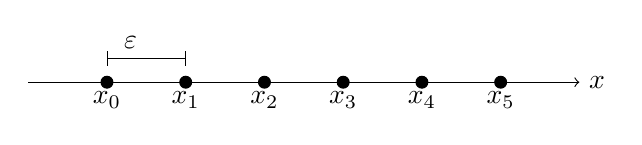
\begin{tikzpicture}
            \draw[->] (-1, 0) -- (6, 0);
            \node[right] at (6, 0) {\(x\)};
            \foreach \x in {0, 1, 2, 3, 4, 5} {
                \draw[fill=black] (\x, 0) circle[radius=0.075cm];
                \node[below] at (\x, 0) {\(x_{\x}\)};
            }
            \draw[|-|] (0, 0.3) -- (1, 0.3);
            \node[above] at (0.3, 0.3) {\(\varepsilon\)};
        \end{tikzpicture}
        \caption{A one dimensional discrete system of \(N = 6\) points, \(x_i\), spaced evenly \(\varepsilon\) apart.}
        \label{fig:one dimensional discrete system}
    \end{figure}
    We can now limit the domain of the wave~function to \(\{x_i\st i=0,\dotsc, 5\}\).
    We define
    \[\psi_i = \sqrt{\varepsilon}\psi(x_i) \in\complex.\]
    We then collect this set of evaluations of \(\psi(x)\) into one object:
    \[
        \ket{\psi} =
        \begin{pmatrix}
            \psi_0\\ \vdots\\ \psi_5
        \end{pmatrix}
    \]
    \(\ket{\psi}\) is a member of a six-dimensional vector space, \(\hilbert\).
    Note that it is wrong to write \(\ket{\psi(x)}\).
    \(\ket{\psi}\) and \(\psi(x)\) are different objects writing \(\ket{\psi(x)}\) is similar to putting a coordinate label on a vector like \(\vv{v}_x\), its just wrong.
    
    \subsubsection{Basis}
    By specifying a vector by its components we assume a basis.
    One such basis is
    \[
        \ket{\xi_0} =
        \begin{pmatrix}
            1\\ 0\\ 0\\ \vdots\\ 0
        \end{pmatrix}
        ,\qquad\ket{\xi_1} =
        \begin{pmatrix}
            0\\ 1\\ 0\\ \vdots\\ 0
        \end{pmatrix}
        ,\dotsc, \ket{\xi_5} =
        \begin{pmatrix}
            0\\ \vdots\\ 0\\ 0\\ 1
        \end{pmatrix}
        .
    \]
    Any vector \(\psi\in\hilbert\) can be written as a linear combination of these basis vectors:
    \[\ket{\psi} = \sum_{k=0}^{5} \psi_k\ket{\xi_k}\]
    where as usual
    \[\psi_k = \braket{\xi_k}{\psi}.\]
    For now we will make some assumptions about extracting physical information from state vectors and wave functions.
    We assume that \(\abs{\psi(x)}^2\) gives the probability density of finding the system at \(x\).
    We also assume that \(\abs{\psi_i}^2 = \varepsilon\abs{\psi(x_i)}^2\) gives the probability of finding the system at \(x_i\).
    Note that the first of these is a probability density and the second is a probability.
    This is because the first is referring to a continuous variable, \(x\), and the second refers to a discrete variable, \(x_i\).
    This is the same as how a probability density function, \(p\), gives a probability, \(p(x)\dd{x}\), here \(\varepsilon\) plays the role of \(\dd{x}\).
    
    With these assumptions we have a physical description of the basis states.
    The vector \(\ket{\xi_i}\) represents a system that is at \(x_i\) with probability 1.
    
    \subsubsection{Scalar Product and Norm}
    We can define a scalar product between \(\ket{\varphi}, \ket{\psi}\in\hilbert\)
    \[\braket{\varphi}{\psi} = \sum_{k=0}^{6} \varphi_k^*\psi_k.\]
    This allows us to induce a norm:
    \[\norm{\psi}^2 = \sum_{k=0}^{6} \abs{\psi_k}^2.\]
    As usual we require state vectors be normalised so
    \[\norm{\psi}^2 = \sum_{k=0}^{6} \abs{\psi_k}^2 = 1.\]
    
    \subsection{Continuous System}
    Moving from this discretised system to a continuous one is as simple as taking the limiting case as \(N \to \infty\) and \(\varepsilon \to 0\).
    After doing this we have that \(\ket{\psi}\in\hilbert_\infty\) where \(\hilbert_\infty\) is an infinite dimensional vector space.
    
    \subsubsection{Basis}
    Define the following basis vectors for our discretised system:
    \[\ket{x_k} = \frac{1}{\sqrt{\varepsilon}}\ket{\xi_k}.\]
    Which gives us \(\ket{\xi_k} = \sqrt{\varepsilon}\ket{x_k}\)
    A vector in the finite dimensional vector space, \(\hilbert\), can be written as
    \[\ket{\psi} = \sum_{k=0}^{N} \psi_k\ket{\xi_k} = \sum_{k=0}^{N} \sqrt{\varepsilon}\psi(x_k)\ket{\xi_k} = \sum_{k=0}^{N} \varepsilon\psi(x_k)\ket{x_k}.\]
    After a limiting process taking \(N\to\infty\) and \(\varepsilon\to 0\) we can write \(\ket{\psi}\in\hilbert_{\infty}\) as
    \[\ket{\psi} = \int\dd{x}\psi(x)\ket{x}\]
    where
    \[\ket{x} = \lim_{\varepsilon\to 0}\frac{1}{\sqrt{\varepsilon}}\ket{\xi_k}.\]
    
    As normal we can find the component, here \(\psi(x)\), with a scalar product with a basis vector:
    \[\psi(x) = \braket{x}{\psi}.\]
    Using this we have
    \[\ket{\psi} = \int\dd{x}\braket{x}{\psi}\ket{x} = \int\dd{x}\ket{x}\braket{x}{\psi}.\]
    We see that \(\ketbra{x}{x}\) is a projection operator and again the completeness relation holds, this time in the form
    \[\int\dd{x}\ketbra{x}{x} = \ident.\]
    
    \subsubsection{Scalar Product and Norm}
    Let \(\ket{\psi}, \ket{\varphi}\in\hilbert\).
    Then their scalar product is
    \[\braket{\varphi}{\psi} = \sum_{k=0}^{N} \varphi_k^*\psi_k = \sum_{k=0}^{N}[\sqrt{\varepsilon}\varphi^*(x_k)][\sqrt{\varepsilon}\psi(x_k)] = \sum_{k=0}^{N}\varepsilon\varphi^*(x_k)\psi(x_k).\]
    After a limiting process taking \(N\to\infty\) and \(\varepsilon\to 0\) we see that for \(\ket{\varphi}, \ket{\psi}\in\hilbert_\infty\) we have
    \[\braket{\varphi}{\psi} = \int\dd{x}\varphi^*(x)\psi(x).\]
    The norm induced by this for \(\ket{\psi}\in\hilbert_\infty\) is given by
    \[\norm{\psi}^2 = \braket{\psi}{\psi} = \int\dd{x}\psi^*(x)\psi(x) = \int\dd{x}\abs{\psi(x)}^2.\]
    For states to be normalisable we require that \(\norm{\psi} < \infty\).
    The space of functions, \(f\colon A\to \complex\), that have this property is called the space of \define{square integrable functions} and is denoted \(\squareIntegrable(A)\).
    For our example of a continuous system we are interested in \(\squareIntegrable(\reals)\).
    If we limit our system to the interval \([a, b]\) where \(a, b\in\reals\) and \(b > a\) then we are interested in the space \(\squareIntegrable([a, b])\).
    
    \subsubsection{Scalar Product of Basis Vectors}
    In the discrete system \(\ket{\xi_k}\) describes a state that is a \(x_k\) with probability 1.
    We want to know what \(\ket{x}\) describes in our continuous case.
    Consider the inner product of two basis states:
    \[\braket{x}{x'} = \lim_{\varepsilon\to 0}\braket{x_k}{x_{k'}} = \lim_{\varepsilon\to 0} \frac{1}{\varepsilon}\braket{\xi_k}{\xi_{k'}}.\]
    Using the orthonormality of \(\{\xi_k\}\) this gives us
    \[
        \braket{x}{x'} = \lim_{\varepsilon\to 0}\frac{1}{\varepsilon}\delta_{kk'} =
        \begin{cases}
            0, & x \ne x',\\
            \infty, &x = x',
        \end{cases}
    \]
    where we have used the fact that if \(x = x'\) then \(\ket{\xi_k} = \ket{\xi_{k'}}\) so \(\delta_{kk'} = \delta_{kk} = 1\) so
    \[\lim_{\varepsilon\to 0} \frac{1}{\varepsilon} = \infty.\]
    On the other hand if \(x \ne x'\) then \(\ket{\xi_k}\ne\ket{\xi_{k'}}\) so \(\delta_{kk'} = 0\).
    Then in the limit we have
    \[\lim_{\varepsilon\to 0}\frac{0}{\varepsilon} = \lim_{\varepsilon\to 0}\frac{\dv{\varepsilon}0}{\dv{\varepsilon}\varepsilon} = \lim_{\varepsilon\to 0}\frac{0}{1} = 0.\]
    We now compute the following integral for reasons that will become clear afterwards:
    \begin{align*}
        \int\dd{x'} f(x')\braket{x}{x'} &= \lim_{\stackrel{N\to \infty}{\varepsilon\to 0}}\sum_{k=0}^{N} \varepsilon f(x_{k'})\braket{x_k}{x_k}\\
        &= \lim_{\stackrel{N\to \infty}{\varepsilon\to 0}}\sum_{k=0}^{N} \varepsilon f(x_{k'})\frac{1}{\varepsilon}\braket{\xi_{k}}{\xi_{k'}}\\
        &= \lim_{N\to\infty}\sum_{k=0}^{N}  f(x_k)\braket{\xi_{k}}{\xi_{k'}}\\
        &= \lim_{N\to\infty} f(x_{k'})\delta_{kk'}\\
        &= \lim_{\varepsilon\to 0}f(x_{k})\\
        &= f(x)
    \end{align*}
    So we see that
    \[\int\dd{x'}f(x')\braket{x}{x'} = f(x)\]
    this, as well as being zero if \(x \ne x'\) defines the \define{Dirac delta distribution}:
    \[
        \delta(x - x') =
        \begin{cases}
            0, & x\ne x',\\
            \infty, & x = x'
        \end{cases}
    \]
    and
    \[\int\dd{x'}f(x')\delta(x - x') = f(x).\]
    So we can identify
    \[\braket{x}{x'} = \delta(x - x').\]
    Using this we get around the fact that \(\{\ket{x}\}\) are not normalisable, that is that \(\braket{x}{x} = \infty\), and we can still extract meaningful information as long as we only have \(\braket{x}{x}\) inside of integrals.
    
    

    \part{Observables}
    \section{Observables}
    In \acrshort{qm} the outcome of a measurement is the outcome of a stochastic variable.
    The theory can only predict the \acrfull{pdf} of the outcome of a given experiment.
    \subsection{Some Statistics}
    A continuous random, or stochastic, variable is one that can take on a different value every time we measure it.
    The values that it can take can be characterised by a \define{\acrfull{pdf}}.
    If \(x\) is a continuous random variable and can take any value in some set \(S\) then the \acrshort{pdf} of \(x\) is a function
    \[p\colon S\to[0, 1]\]
    such that the probability that \(x\) is between \(x\) and \(x + \dd{x}\) is given by \(p(x)\dd{x}\).
    Using this we have that the probability that \(x\) is in the interval \(\mathcal{I} = [a, b]\) is
    \[P(x\in\mathcal{I}) = \int_a^b \dd{x} p(x).\]
    Since probabilities should add up to one we require \(p\) to be properly normalised so that
    \[P(x\in S) = \int_S\dd{x}p(x) = 1.\]
    As a way of characterising a \acrshort{pdf} we define its \define{\(\mathdefine{n}\)th moment} as
    \[\mu_n = \int\dd{x}p(x)x^n.\]
    Clearly if \(p\) is properly normalised then \(\mu_0 = 1\).
    The \define{mean} value of the random variable, \(x\), is
    \[\mu_1 = \expected{x} = \int\dd{x}p(x)x.\]
    The \define{variance} of the variable, \(x\), is
    \[\Var[x] = \mu_2 - (\mu_1)^2 = \expected{x^2} - \expected{x}^2.\]
    
    \subsection{Position Operator}
    The state of the system is described by \(\psi(x) = \braket{x}{\psi}\) where \(\ket{\psi}\in\hilbert\), with \(\hilbert\) being some infinite dimensional vector space that has \(\{\ket{x}\}\) as a basis.
    The \acrshort{pdf} for finding a system in the state \(\ket{\psi}\in\hilbert\) at position \(x\) is
    \[p(x) = \abs{\psi(x)}^2.\]
    The \define{expected value} of \(x\) is
    \[\expected{x} = \int_{-\infty}^{\infty} \dd{x}p(x)x.\]
    We introduce an operator, \(\operator{X}\colon\hilbert\to\hilbert\), defined by
    \[\bra{x}\operator{X}\ket{\psi} = x\braket{x}{\psi},\]
    or, equivalently,
    \[\operator{X}\psi(x) = x\psi(x).\]
    This allows us to write the mean value as
    \begin{align*}
        \expected{x} &= \int\dd{x}\abs{\psi(x)}^2x\\
        &= \int\dd{x}\psi(x)^*x\psi(x)\\
        &= \int\dd{x}\braket{\psi}{x}x\braket{x}{\psi}\\
        &= \int\dd{x}\braket{\psi}{x}\bra{x}\operator{X}\ket{\psi}\\
        &= \bra{\psi}\operator{X}\ket{\psi}\\
        &= \expected{\operator{X}}.
    \end{align*}
    Here we used the completeness relation to get rid of the integral and projection operators.
    Note that \(\expected{\operator{X}}\) is just a short hand for \(\bra{\psi}\operator{X}\ket{\psi}\) when the state \(\psi\) is clear.
    It is not the expected value of the operator \(\operator{X}\) per se but the expected value of \(x\) which is in some way related to the operator \(\operator{X}\).
    
    There is a theorem that states that if we know all the moments of a \acrshort{pdf} then this uniquely determines the \acrshort{pdf}.
    We can find the \(n\)th moment fairly easily:
    \begin{align*}
        \bra{\psi}\operator{X}^n\ket{\psi} &= \int \dd{x} \braket{\psi}{x}\bra{x}\operator{X}^n\ket{\psi}\\
        &= \int \dd{x} \braket{\psi}{x}x^n\braket{x}{\psi}\\
        &= \int \dd{x} \psi(x)^* x^n \psi(x)\\
        &= \int \dd{x} \abs{\psi(x)}^2x^n\\
        &= \int \dd{x} p(x)x^n\\
        &= \mu_n.
    \end{align*}
    So by taking the matrix elements of \(\operator{X}^n\) we can fully describe the \acrshort{pdf}.
    
    Here we have used the following theorem.
    \begin{theorem}{}{op^n ket = eigenvalue^n ket}
        If \(\operator{O}\colon\hilbert\to\hilbert\) is an operator and acts on \(\ket{\psi}\in\hilbert\) as \(\operator{O}\ket{\psi} = z\ket{\psi}\) where \(z\in\complex\) then \(\operator{O}^n\ket{\psi} = z^n\ket{\psi}\).
    \end{theorem}
    \begin{proof}
        We will prove this by induction.
        The basis case of \(n = 0\) holds as by definition \(\operator{O}^0 = \ident\) so
        \[\operator{O}^0\ket{\psi} = \ident\ket{\psi} = \ket{\psi} = 1\ket{\psi} = z^0\ket{\psi}.\]
        Now suppose that this holds for \(n = k\), that is
        \[\operator{O}^k\ket{\psi} = z^k\ket{\psi}.\]
        Then
        \begin{align*}
            \operator{O}^{k+1}\ket{\psi} &= \operator{O}(\operator{O}^k\ket{\psi})\\
            &= \operator{O}(z^k\ket{\psi})\\
            &= z^k(\operator{O}\ket{\psi})\\
            &= z^k(z\ket{\psi})\\
            &= z^{k+1}\ket{\psi}.
        \end{align*}
        So it holds for \(n = k + 1\).
        Thus by induction this holds for all \(n \in\naturals\).
    \end{proof}
    
    \subsection{Generic Observables}
    We define an \define{observable} as a quantity that can be measured in an experiment.
    Here an experiment is a black box that we provide somehow with a prepared state, \(\ket{\psi}\), and after the experiment we are given a value for the observable that we were measuring.
    One important thing that we assume is that the experiment is reproducible, that is that we can prepare the system in the same way and perform the same measurement as many times as needed.
    
    This gives rise to the second postulate of \acrshort{qm}:
    \begin{postulate}{}{}
        In quantum mechanics each observable, \(O\), is associated to a linear operator, \(\operator{O}\colon\hilbert\to\hilbert\).
    \end{postulate}
    The naive approach to find the expected value of an observable, \(O\), given a specific state, \(\ket{\psi}\), might be to try \(\operator{O}\ket{\psi}\).
    However this gives us another vector and we expect real numbers as the results of measurements.
    It turns out that the expected value of \(O\) for a system in the state \(\ket{\psi}\) is given by the matrix elements of \(\operator{O}\):
    \[\expected{O} = \bra{\psi}O\ket{\psi}.\]
    
    \subsubsection{Observing Observables}
    When we say that the value of an observable \(O\) is a stochastic variable is that if we set up the system in state \(\ket{\psi}\) and measure \(O\) and get a result \(O^{(1)}\), and then set up the system in state \(\ket{\psi}\) and measure \(O\) and get a result \(O^{(2)}\), and so on, then we end up with a set of values \(\{O^{(1)}, O^{(2)}, \dotsc, O^{(n)}\}\).
    The important thing is that it is possible that \(O^{(i)}\ne O^{(j)}\), even accounting for experimental error.
    This is very different to classical mechanics where we would expect that a measurement gives the same result every time, up to some level of precision.
    
    The expectation value of \(O\) is then
    \[\expected{O} = \lim_{n\to\infty} \frac{1}{n}\sum_{k=1}^{n} O^{(k)}.\]
    So far we have focused on the value of the observable but with \acrshort{qm} we can predict more than this.
    Given an observable, \(O\), we can predict
    \begin{itemize}
        \item the possible outcomes of a measurement of \(O\),
        \item the probability of obtaining each of these possible outcomes.
    \end{itemize}
    All questions in \acrshort{qm} need to be phrased in terms of possible outcomes and their probabilities, these are the only things that the theory predicts.
    
    \subsection{Eigenvalues and Eigenstates}
    The possible outcomes of measuring an observable, \(O\), are given by the third postulate of \acrshort{qm}:
    \begin{postulate}{}{}
        When measuring an observable, \(O\), the possible outcomes, \(O_k\), are the eigenvalues of the operator, \(\operator{O}\).
    \end{postulate}
    If \(\operator{O}\colon\hilbert\to\hilbert\) and \(\ket{\psi_k}\in\hilbert\) then \(\ket{\psi_k}\) is an \define{eigenvector} or \define{eigenstate} with \define{eigenvalue} \(O_k\) if these are solutions to the following:
    \[\operator{O}\ket{\psi_k} = O_k\ket{\psi_k}.\]
    That is the only result of \(\operator{O}\) when acting on \(\ket{\psi_k}\) is to scale \(\ket{\psi_k}\) by some amount.
    In general in a complex vector space eigenvalues are complex, we will see later that this does not give rise to the correct physics.
    
    If \(O_k\) is an eigenvalue of the operator, \(\operator{O}\), then we say that \(O_k\) is \(g\)-fold degenerate if there are exactly \(g\) linearly independent eigenvectors, \(\ket{u_k^{(n)}}\in\hilbert\) such that
    \[\operator{O}\ket{u_k^{(n)}} = O_k\ket{u_k^{(n)}}\]
    for \(n = 1, \dotsc, g\).
    That is that \(O_k\) is an eigenvalue for \(g\) fundamentally different eigenvectors (as opposed to scaled versions of the same eigenvector).
    
    Any linear combination of the form
    \[\sum_{n=1}^{g}c_n\ket{u_k^{(n)}}\]
    where \(c_k\in\complex\) is also an eigenstate of \(\operator{O}\), this is fairly easy to show using the linearity of \(\operator{O}\):
    \begin{align*}
        \operator{O}\sum_{n=1}^{g}c_n\ket{u_k^{(n)}} &= \sum_{n=1}^{g}c_n\operator{O}\ket{u_k^{(n)}}\\
        &= \sum_{n=1}^{g}c_nO_k\ket{u_k^{(n)}}\\
        &= O_k\sum_{n=1}^{g}c_n\ket{u_k^{(n)}}.
    \end{align*}
    In fact any set of eigenvectors with degenerate eigenvalues forms a \(g\)-dimensional vector subspace of \(\hilbert\).
    
    One logical question that we may ask now is what do the eigenstates represent?
    We can try to measure the expected value of \(O\) in a system that is the state \(\ket{\psi_k}\) which is an eigenstate of \(\operator{O}\) with eigenvalue \(O_k\).
    We get
    \begin{align*}
        \expected{O} &= \bra{\psi_k}\operator{O}\ket{\psi_k}\\
        &= \bra{\psi_k}O_k\ket{\psi_k}\\
        &= O_k\braket{\psi_k}{\psi_k}\\
        &= O_k.
    \end{align*}
    So the expected value of \(O\) measured on its eigenstate, \(\ket{\psi_k}\), is \(O_k\).
    We can also compute the variance:
    \begin{align*}
        \Var_{\psi_k}[O] &= \expected{O^2} - \expected{O}^2\\
        &= \bra{\psi_k}\operator{O}^2\ket{\psi_k} - [\bra{\psi_k}\operator{O}\ket{\psi_k}]^2\\
        &= \bra{\psi_k}O_k^2\ket{\psi_k} - [\bra{\psi_k}O_k\ket{\psi_k}]^2\\
        &= O_k^2\braket{\psi_k}{\psi_k} - [O_k\braket{\psi_k}{\psi_k}]^2\\
        &= O_k^2 - O_k^2\\
        &= 0.
    \end{align*}
    where we have used the result of theorem~\ref{thm:op^n ket = eigenvalue^n ket}, which states \(\operator{O}^2\ket{\psi_k} = O_k^2\ket{\psi_k}\) so
    \[\bra{\psi_k}\operator{O}^2\ket{\psi_k} = \bra{\psi_k}O_k^2\ket{\psi_k} = O_k^2\braket{\psi_k}{\psi_k}.\]
    The important thing is that the expected value is \(O_k\) and the variance is zero.
    This means that there is no spread in the values measured and so \(O^{(i)} = O_k\) for all \(i\).
    This means that in the state \(\ket{\psi_k}\) when we measure \(O\) we get \(O_k\) with probability 1.
    
    \subsection{Hermitian Operators}
    \subsubsection{Hermitian Conjugate}
    Let \(\operator{O}\colon\hilbert\to\hilbert\).
    Then we define the \define{hermitian conjugate} of \(\operator{O}\), denoted \(\operator{O}\hermit\), to be another operator, \(\operator{O}\hermit\colon\hilbert\to\hilbert\), defined such that for all \(\ket{\varphi}, \ket{\psi}\in\hilbert\)
    \[\bra{\varphi}\operator{O}\hermit\ket{\psi} = [\bra{\psi}\operator{O}\ket{\varphi}]^*.\]
    Compare this to the usual linear algebra definition:
    \[O_{ij}\hermit = O_{ji}^*.\]
    We see that since \(\bra{\varphi}\operator{O}\hermit\ket{\psi}\) gives the matrix elements of \(\operator{O}\hermit\) these two definitions are equivalent.
    
    \begin{example}\label{exa:hermitian conjugate of the derivative}
        Consider the operator \(\operator{O} = \dv{x}\) defined by
        \begin{align*}
            \bra{x}\operator{O}\ket{\psi} &= \bra{x}\dv{x}\ket{\psi}\\
            &= \dv{x}\braket{x}{\psi}\\
            &= \dv{x}\psi(x).
        \end{align*}
        Compute \(\operator{O}\hermit\).
        \begin{align*}
            \bra{\varphi}\operator{O}\hermit\ket{\psi} &= [\bra{\psi}\operator{O}\ket{\varphi}]^*
            \shortintertext{inserting completeness gives}
            &= \left[ \int_{-\infty}^{\infty} \dd{x} \braket{\psi}{x}\bra{x}\operator{O}\ket{\varphi} \right]^*\\
            &= \left[ \int_{-\infty}^{\infty} \dd{x} \psi(x)^*\dv{x}\varphi(x) \right]^*.\stepcounter{equation}\tag{\theequation}\label{eqn:int psi d/dx phi}
        \end{align*}
        We can now integrate by parts:
        \[
            \begin{array}{ll}
                u = \psi(x)^*, & v = \varphi(x),\\
                u' = \dv{x}\psi(x)^*, & v' = \dv{x}\varphi(x).
            \end{array}
        \]
        \begin{align*}
            \bra{\varphi}\operator{O}\hermit\ket{\psi} &= \left[ [\psi(x)^*\varphi(x)]_{-\infty}^{\infty} - \int_{-\infty}^{\infty} \dd{x} \varphi(x)\dv{x}\psi(x)^* \right]^*
            \shortintertext{this first term is zero as \(\psi\) and \(\varphi\) are wave functions so are square integrable so they vanish at infinity leaving us with}
            &= \left[ -\int_{-\infty}^{\infty} \dd{x} \varphi(x)\dv{x}\psi(x)^* \right]^*\\
            &= -\int_{-\infty}^{\infty} \dd{x} \varphi(x)^*\dv{x}\psi(x)\\
            &= -\int_{-\infty}^{\infty} \dd{x} \braket{\varphi}{x}\bra{x}\operator{O}\ket{\psi}\\
            &= -\bra{\varphi}\operator{O}\ket{\psi}.
        \end{align*}
        So we can identify
        \[\left(\dv{x}\right)\hermit = -\dv{x}.\]
    \end{example}
    
    \subsubsection{Hermitian Operator}
    An operator, \(\operator{O}\colon\hilbert\to\hilbert\), is \define{hermitian} if \(\operator{O}\hermit = \operator{O}\).
    We saw in example~\ref{exa:hermitian conjugate of the derivative} that \(\dv{x}\) is \emph{not} hermitian as \(\operator{O}\hermit = -\operator{O}\), this property is actually called being \define{anti-hermitian}.
    \begin{example}\label{exa:momentum operator hermitian}
        Show that \(\operator{O} = -i\hbar\dv{x}\) is hermitian.
        This operator will be important later.
        \begin{align*}
            \bra{\varphi}\operator{O}\hermit\ket{\psi} &= [\bra{\psi}\operator{O}\ket{\varphi}]^*\\
            &= \left[ \int_{-\infty}^{\infty} \dd{x} \braket{\psi}{x}\bra{x}\operator{O}\ket{\varphi} \right]^*\\
            &= \left[ \int_{-\infty}^{\infty} \dd{x} \psi(x)\left(-i\hbar\dv{x}\right) \ket{\varphi}\right]^*\\
            &= \left[ -i\hbar\int_{-\infty}^{\infty} \dd{x} \psi(x)\dv{x} \varphi(x)\right]^*\\
            &= i\hbar \int_{-\infty}^{\infty} \dd{x} \psi(x)^*\dv{x}\varphi(x)\\
            \shortintertext{see equation~\ref{eqn:int psi d/dx phi} for how to do this integral}
            &= -i\hbar \int_{-\infty}^{\infty} \dd{x} \varphi(x)^*\dv{x}\psi(x)\\
            &= \int_{-\infty}^{\infty} \dd{x} \varphi(x)^*\left(-i\hbar\dv{x}\right) \psi(x)\\
            &= \int_{-\infty}^{\infty} \dd{x} \braket{\varphi}{x}\bra{x}\operator{O}\ket{\psi}\\
            &= \bra{\varphi}\operator{O}\ket{\psi}.
        \end{align*}
        So we can identify that
        \[\left(-i\hbar\dv{x}\right)\hermit = -i\hbar\dv{x}\]
        so this is a hermitian operator.
    \end{example}
    \subsubsection{Properties of Hermitian Operators}
    The following important properties of hermitian operators make incredibly important to \acrshort{qm}:
    \begin{enumerate}
        \item Hermitian operators have real eigenvalues.
        That is if \(\operator{O}\colon\hilbert\to\hilbert\) and
        \[\operator{O}\ket{\psi_k} = O_k\ket{\psi_k}\]
        then
        \[\operator{O} = \operator{O}\hermit \implies O_k\in\reals.\]
        
        \item The eigenstates of a hermitian operator that belong to different eigenvalues are orthogonal.
        That is if \(\operator{O}\colon\hilbert\to\hilbert\),
        \[\operator{O}\ket{\psi_k} = O_k\ket{\psi_k}, \qquad\text{and}\qquad \operator{O}\ket{\psi_l} = O_l\ket{\psi_l}\]
        where \(O_k \ne O_l\) then
        \[\braket{\psi_k}{\psi_l} = 0.\]
        
        \item If \(\operator{O}\colon\hilbert\to\hilbert\) then there exists an orthogonal basis of \(\hilbert\) made of eigenvectors of \(\operator{O}\).
        In other words \(\ket{\psi}\in\hilbert\) can be written as
        \[\ket{\psi} = \sum_k c_k\ket{\psi_k}\]
        where \(c_k\in\complex\) are given by
        \[c_k = \braket{\psi_k}{\psi}.\]
    \end{enumerate}
    We can prove these fairly easily:
    \begin{theorem}{}{}
        Hermitian operators have real eigenvalues.
    \end{theorem}
    \begin{proof}
        Suppose \(\operator{O}\) is a hermitian operator on \(\hilbert\).
        Let \(\ket{\psi_k}\) be a normalised eigenvector of \(\operator{O}\) with eigenvalue \(O_k\).
        Then
        \[\operator{O}\ket{\psi_k} = O_k\ket{\psi_k}.\]
        Taking an inner product with \(\bra{\psi_k}\) we get
        \begin{equation}\label{eqn:psi_k O psi_k = O_k}
            \bra{\psi_k}\operator{O}\ket{\psi_k} = \bra{\psi_k}O_k\ket{\psi_k} = O_k\braket{\psi_k}{\psi_k} = O_k
        \end{equation}
        where we have used the fact that \(\ket{\psi_k}\) is normalised so \(\braket{\psi_k}{\psi_k} = 1\).
        Taking the complex conjugate of this equation gives us
        \[[\bra{\psi_k}\operator{O}\ket{\psi_k}]^* = O_k^*.\]
        Using the definition of the hermitian conjugate the left hand side is equivalent to
        \[\bra{\psi_k}\operator{O}\hermit\ket{\psi_k}.\]
        Since \(\operator{O}\) is hermitian this in turn is equivalent to
        \[\bra{\psi_k}\operator{O}\ket{\psi_k},\]
        which, as we saw in equation~\ref{eqn:psi_k O psi_k = O_k}, is just \(O_k\).
        This means that we have
        \[O_k = O_k^*\]
        which can only be true if \(O_k\in\reals\).
    \end{proof}
    \begin{theorem}{}{}
        The eigenfunctions of a hermitian operator which belong to different eigenvalues are orthogonal.
    \end{theorem}
    \begin{proof}
        Let \(\operator{O}\) be an operator on \(\hilbert\).
        Suppose that
        \[\operator{O}\ket{\psi_1} = O_1\ket{\psi_1}, \qquad\text{and}\qquad \operator{O}\ket{\psi_2} = O_2\ket{\psi_2}\]
        where \(O_1 \ne O_2\).
        Taking the inner product of the first of these equations with \(\bra{\psi_2}\) we have
        \begin{equation}\label{eqn:psi_2 O psi_1 = O_1 psi_2 psi_1}
            \bra{\psi_2}\operator{O}\ket{\psi_1} = O_1\braket{\psi_2}{\psi_1}.
        \end{equation}
        Instead taking the inner product of the second equation with \(\bra{\psi_1}\) we have
        \[\bra{\psi_1}\operator{O}\ket{\psi_2} = O_2\braket{\psi_1}{\psi_2}.\]
        Taking the complex conjugate, using the definition of the hermitian conjugate, and then using the fact that \(\operator{O}\hermit = \operator{O}\) the left hand side of the above equation gives us
        \[[\bra{\psi_1}\operator{O}\ket{\psi_2}]^* = \bra{\psi_2}\operator{O}\hermit\ket{\psi_1} = \bra{\psi_2}\operator{O}\ket{\psi_1}.\]
        The right hand side gives
        \[O_2^*\braket{\psi_1}{\psi_2} = O_2\braket{\psi_1}{\psi_2},\]
        where we have used the fact that \(\operator{O}\) is hermitian so its eigenvalues are real and therefore \(O_2^* = O_2\).
        Comparing this with equation~\ref{eqn:psi_2 O psi_1 = O_1 psi_2 psi_1} we see that
        \[O_2\braket{\psi_2}{\psi_1} = O_1\braket{\psi_2}{\psi_1}\]
        which gives us
        \[(O_2 - O_1)\braket{\psi_2}{\psi_1} = 0.\]
        Given that \(\complex\) is a field and so has no zero divisors either \(O_2 - O_1 = 0\) or \(\braket{\psi_2}{\psi_1} = 0\).
        By our assumption \(O_2 - O_1\ne 0\) so we must have \(\braket{\psi_2}{\psi_1} = 0\).
        This means that \(\ket{\psi_1}\) and \(\ket{\psi_2}\) are orthogonal.
    \end{proof}
    
    The reason that the first of these properties, that the eigenvalues are real, is important is that we expect real results from an experiment and therefore it only makes sense to have the eigenvalues of an observable be real.
    The other two properties become useful when doing theory as working in the basis given by the eigenvectors, called the eigenbasis, can simplify a lot of equations.
    The process of moving into this eigenbasis is called spectral decomposition.
    
    \subsubsection{Spectral Decomposition}
    \begin{postulate}{}{}
        An observable, \(O\), has an associated hermitian linear operator, \(\operator{O}\colon\hilbert\to\hilbert\), which has a nondegenerate eigenvalue \(O_k\) and associated eigenvector \(\ket{\psi_k}\).
        Given a normalised state, \(\ket{\psi}\in\hilbert\), the probability of measuring \(O\) to be \(O_k\) is
        \[P_k = \abs{c_k}^2 = \abs{\braket{\psi_k}{\psi}}^2\]
        where \(c_k\in\complex\) are the coordinates of \(\ket{\psi}\) in the basis made of the eigenvectors of \(\operator{O}\):
        \[\ket{\psi} = \sum_{k}c_k\ket{\psi_k}.\]
        In the case that \(O_k\) is \(g\)-fold degenerate and has the vectors \(\{\ket{u_k^{(n)}}\}\) as its eigenvectors then the probability of measuring \(O\) to be \(O_k\) is instead the sum of the contributions from the whole subspace spanned by \(\{\ket{u_k^{(n)}}\}\):
        \[P_k = \sum_{n=1}^{g} \abs{\braket{u_k^{(n)}}{\psi}}^2.\]
    \end{postulate}
    This postulate is the reason that we require states be normalised because this means that
    \[\sum_k P_k = \sum_k\sum_{n=1}^{g_k}\abs{\braket{u_k^{(n)}}{\psi}}^2 = 1,\]
    where \(g_k\) is the degeneracy of the eigenvalue \(O_k\).
    In the case of non-degenerate eigenvalues the second sum has only one term and we recover the more familiar requirement that
    \[\sum_k \abs{\braket{\psi_k}{\psi}}^2 = 1.\]
    
    
    \section{Collapse of the State Vector}
    Suppose we have a state \(\ket{\psi}\) and we measure the observable \(O\) and get a value of \(O_k\) which has the associated eigenvector \(\ket{\psi_k}\).
    Immediately after performing this measurement we know that the value of \(O\) is \(O_k\) with probability 1.
    This must mean that the system is in state \(\ket{\psi_k}\).
    The act of measuring changes the state of the system.
    This is true for all measurements we could make.
    \begin{postulate}{}{}
        Immediately after a measurement that gives the result \(O_k\), where \(O_k\) is a non-degenerate eigenvalue of \(\operator{O}\), the state of the system is \(\ket{\psi_k}\), which is the eigenvector associated with \(O_k\).
        The state vector has been projected onto the eigenstate by the process of performing the measurement.
    \end{postulate}
    Mathematically what this looks like is we start with a state, \(\ket{\psi}\), and perform some sort of measurement.
    The outcome of the measurement is \(O_k\) with probability \(\abs{\braket{\psi_k}{\psi}}^2\).
    After the experiment the state is
    \[\frac{1}{\sqrt{\bra{\psi}\operator{\proj}_k\ket{\psi}}}\operator{\proj}_k\ket{\psi}.\]
    Here \(\operator{\proj}_k = \ketbra{\psi_k}{\psi_k}\) is the projection operator onto the eigenspace of \(\ket{\psi_k}\).
    
    If instead \(O_k\) has degeneracy \(g_k\) then
    \[\operator{\proj}_k = \sum_{n=1}^{g_k} \ketbra{u_k^{n}}{u_k^{(n)}}\]
    where \(\ket{u_k^{(n)}}\) are the eigenvectors with eigenvalue \(O_k\) for \(n = 1, \dotsc, g_k\).
    The state after measurement is then
    \[\frac{1}{\sqrt{\sum_{n=1}^{g_k}\abs{c_k^{(n)}}^2}} \sum_{n=1}^{g_k}c_k^{(n)} \ket{u_k^{(n)}}.\]
    
    \subsection{Compatible Observables}
    Suppose \(A\) and \(B\) are observables.
    If we take three measurements, first measuring \(A\), then \(B\), then \(A\) again, \(A\) and \(B\) are said to be \define{compatible} if and only if the result of the third measurement is equal to the result of the first measurement with probability one.
    That is measuring \(B\) doesn't change the outcome of measuring \(A\).
    
    Suppose that \(A\) and \(B\) have associated operators \(\operator{A}\) and \(\operator{B}\) respectively, which have no degenerate eigenvalues.
    Suppose also that
    \[\operator{A}\ket{u_i} = A_i\ket{u_i}, \qquad\text{and}\qquad \operator{B}\ket{v_i} = B_i\ket{v_i}.\]
    After we measure \(A\) if we get a value of \(A_j\) then the state of the system is \(\ket{u_j}\).
    Next we measure \(B\) and we get \(B_k\) meaning that the system is in the state \(\ket{v_k}\).
    The only way that we can guarantee another measurement of \(A\) will yield the same value as the first is if \(\ket{v_k} = \ket{u_j}\).
    For this to hold for all possible values of the measurement we must have that \(\ket{v_k} = \ket{v_j}\) for all possible values of \((i, j)\).
    If there is no degeneracy then we have a one to one correspondence between eigenvectors of \(\operator{A}\) and eigenvectors of \(\operator{B}\).
    We say that \(\operator{A}\) and \(\operator{B}\) have a common eigenbasis.
    
    The conditions under which \(A\) and \(B\) are compatible are summarised in the compatibility theorem:
    \begin{theorem}{The Compatibility Theorem}{}
        Given two observables, \(A\) and \(B\), with associated operators \(\operator{A}\) and \(\operator{B}\), then the following are equivalent:
        \begin{enumerate}
            \item \(A\) and \(B\) are compatible observables,
            \item \(\operator{A}\) and \(\operator{B}\) have a common eigenbasis,
            \item The operators \(\operator{A}\) and \(\operator{B}\) commute: \([\operator{A}, \operator{B}] = 0\).
        \end{enumerate}
    \end{theorem}
    Due to the third condition compatible observables are sometimes called \define{commuting observables}.
    
    \subsection{Complete Sets of Compatible observables}
    Consider an observable \(A\) with associated operator \(\operator{A}\).
    Let the eigenbasis of \(\operator{A}\) be \(\{u_i\}\).
    In the case of no degeneracy we have
    \[\operator{A}\ket{u_k} = a_k\ket{u_k}.\]
    We can identify the eigenvector \(\ket{u_k}\) by its eigenvalue, which we do by writing it \(\ket{a_k}\).
    \(A\) is then trivially a \gls{csco} by itself.
    
    In the case where there is degeneracy we can introduce another observable, \(B\), which is compatible with \(A\).
    It is possible to find a common eigenbasis of \(\operator{A}\) and \(\operator{B}\).
    Call this eigenbasis \(\{\ket{v_k^{(n)}}\}\) where \(n=1,\dotsc, g_k\).
    Suppose that
    \[\operator{A}\ket{v_k^{(n)}} = a_i\ket{v_k^{(n)}}, \qquad\text{and}\qquad \operator{B}\ket{v_k^{(n)}} = b_j\ket{v_k^{(n)}}.\]
    If \((a_i, b_j)\) uniquely identifies this eigenstate then \(A\) and \(B\) are a \gls{csco}.
    We then write \(\ket{v_{k}^{(n)}} = \ket{a_i, b_j}\).
    
    If \((a_i, b_j)\) does not uniquely identify \(\ket{v_k^{(n)}}\) then we simply keep introducing observables that are compatible with all previously introduced observables until we have a tuple of eigenvalues that does uniquely identify each eigenvector.
    
    That is \(\{A, B, C, \dotsc\}\) is a \define{\acrfull{csco}} if and only if:
    \begin{itemize}
        \item All observables commute in pairs,
        \item Specifying all the eigenvalues of the operators identifies a unique eigenvector in the common eigenbasis.
    \end{itemize}

    Given a \gls{csco}, for example, \(\{A, B, C\}\), we can expand a state in the common eigenbasis as
    \[\ket{\psi} = \sum_{n, p, q}c_{npq}\ket{a_n,b_p,c_q}.\]
    The probability of measuring \(a_n\), \(b_p\), and \(c_q\) simultaneously is then \(\abs{c_{npq}}^2\).
    
    \section{Continuous Spectra}
    Up to now we have only considered eigenvalues and eigenvectors that can be identified by a discrete variable, \(k\).
    We can also have eigenvalues that are represented by a continuous variable, \(f\).
    For example
    \[\operator{f}\ket{f} = f\ket{f}\]
    where we follow the convention of identifying an eigenvector by the associated eigenvalue.
    Assuming that \(\operator{f}\) is hermitian then \(f\in\reals\).
    The completeness relation for a continuous basis set is
    \[\int\dd{f}\ketbra{f}{f} = \ident.\]
    We can expand a generic state, \(\ket{\psi}\), in this basis:
    \[\ket{\psi} = \int\dd{f} c(f)\ket{f}.\]
    Here \(c(f)\) plays the role of the coordinates of \(\ket{\psi}\) in the same way that \(c_k\) did in the discrete case.
    The method for computing \(c(f)\) is the same as in the discrete case:
    \begin{align*}
        c(f) &= \braket{f}{\psi}\\
        &= \int\dd{x} \braket{f}{x}\braket{x}{\psi}\\
        &= \int\dd{x} f^*(x)\psi(x).
    \end{align*}
    Since we now have a continuous variable the probability of any one particular value has to be zero.
    However \(\abs{c(f)}^2\) does give the probability density such that
    \[P(f\in[f_-, f_+]) = \int_{f_-}^{f_+} \dd{f} \abs{c(f)}^2.\]
    To be properly normalised we demand that
    \[\int_{-\infty}^{\infty} \dd{f}\abs{c(f)}^2 = 1.\]
    
    Perhaps the most common continuous observable to consider is the position.
    The operator for position is \(\operator{X}\) and its action on \(\ket{\psi}\) is
    \[\operator{X}\ket{\psi} = x\ket{\psi}.\]
    Note that this is \emph{not} an eigenvalue equation, \(x\) is a variable not a constant and this holds for all \(\ket{\psi}\).
    This is simply a statement that the action of \(\operator{X}\) is to multiply the state by \(x\).
    The effect that this has on the wave function is as we would expect:
    \begin{align*}
        \operator{X}\ket{\psi} &= \operator{X}\left[\int\dd{x} \psi(x)\ket{x}\right]\\
        &= \int\dd{x} \psi(x)\operator{X}\ket{x}\\
        &= \int\dd{x} \psi(x)x\ket{x}\\
        &= \int\dd{x} \varphi(x)\ket{x}\\
        &= \ket{\varphi}
    \end{align*}
    where \(\ket{\varphi}\) is defined to be such that \(\braket{x}{\varphi} = \varphi(x) = x\psi(x)\).
    Being slightly lazy with notation we will sometimes write things like
    \[\operator{X}\psi(x) = x\psi(x)\]
    which is not, strictly speaking, defined as operators can only act on elements of \(\hilbert\), not on the coordinates of these vectors.
    However the meaning should be clear enough that it doesn't matter.
    
    \subsection{Orthonormality}
    Suppose that \(f\) and \(f'\) distinct eigenvalues of \(\operator{f}\).
    Then by definition
    \[\operator{f}\ket{f} = f\ket{f},\qquad\text{and}\qquad \operator{f}\ket{f'} = f'\ket{f'}.\]
    We can compute matrix elements of \(\operator{f}\):
    \[\bra{f'}\operator{f}\ket{f} = f\braket{f'}{f},\]
    or using the hermitian property of \(\operator{f}\):
    \begin{align*}
        \bra{f'}\operator{f}\ket{f} &= (\bra{f}\operator{f}\hermit\ket{f'})^*\\
        &= (\bra{f}\operator{f}\ket{f'})^*\\
        &= (f'\braket{f}{f'})^*\\
        &= {f'}^*(\braket{f}{f'})^*\\
        &= f'\braket{f'}{f}.
    \end{align*}
    Hence
    \[(f - f')\braket{f'}{f} = 0.\]
    Assuming that \(f \ne f'\) then \(f - f' \ne 0\) so \(\braket{f'}{f} = 0\).
    
    Consider the state \(\ket{\psi}\) expanded in this basis:
    \[\ket{\psi} = \int\dd{f} c(f)\ket{f}.\]
    We can compute \(\norm{\psi}\):
    \begin{align*}
        \norm{\psi}^2 &= \braket{\psi}{\psi}\\
        &= \int\dd{f'}f^*(f')\bra{f'}\int\dd{f}c(f)\ket{f}\\
        &= \int\dd{f'}\dd{f}c^*(f)c(f)\braket{f'}{f}\\
        &= \int\dd{f}c^*(f)c(f)\braket{f}{f}\\
        &= \int\dd{f}\abs{c(f)}^2\braket{f}{f}
    \end{align*}
    Here we have used that \(\braket{f'}{f}\) is zero apart from when \(f = f'\) to replace \(f'\) with \(f\) while removing one of the integrals.
    We also require that \(\norm{\psi} = 1\) and we already have that
    \[\int\abs{c(f)}^2 = 1\]
    so we must have
    \[\int\dd{f}\braket{f}{f} = 1.\]
    The properties that we have described so far for \(\braket{f'}{f}\) are exactly the definition of the Dirac delta function:
    \[\braket{f'}{f} = \delta(f - f').\]
    
    \begin{example}
        Consider a system on a line.
        The position operator, \(\operator{X}\), is defined as
        \[\operator{X}\ket{x} = x\ket{x}.\]
        A generic state is
        \[\ket{\psi} = \int\dd{x}\psi(x)\ket{x}\]
        where
        \[\psi(x) = \braket{x}{\psi}.\]
        By definition
        \[\braket{x}{x'} = \delta(x - x').\]
        Thus
        \begin{align*}
            \braket{\psi}{\psi} &= \int\dd{x}\dd{x'}\psi^*(x)\psi(x')\braket{x}{x'}\\
            &= \int\dd{x}\dd{x'}\psi^*(x)\psi(x')\delta(x - x')\\
            &= \int\dd{x}\psi^*(x)\psi(x)\\
            &= \int\dd{x}\abs{\psi(x)}^2.
        \end{align*}
        Consider now the state that has a wave function given by
        \[\psi(x) = c\exp\left[\frac{i}{\hbar}p_0x - \frac{(x - x_0)^2}{2\xi^2}\right]\]
        where \(x_0\), \(p_0\), and \(\xi\) are constants and \(c\in\reals\) is a normalisation factor.
        \begin{align*}
            \braket{\psi}{\psi} &= \int_{-\infty}^{\infty} \abs{\psi(x)}^2\\
            &= \int_{-\infty}^{\infty} c^2\exp\left[-\frac{(x - x_0)^2}{2\xi^2}\right]\\
            &= c^2\xi\sqrt{\pi}.
        \end{align*}
        Requiring a normalised state we then have
        \[c = \frac{1}{\pi^{1/4}\sqrt{\xi}}.\]
        The expected position is given by
        \begin{align*}
            \expected{x} &= \int\dd{x} x\abs{\psi(x)}^2\\
            &= \frac{1}{\xi\sqrt{\pi}}\int\dd{x} x\exp\left[-\frac{(x - x_0)^2}{2\xi^2}\right]\\
            &= x_0.
        \end{align*}
        Similarly it can be shown that
        \[\expected{\Delta x^2} = \expected{(x - x_0)^2} = \xi^2.\]
        This can be shown by computing the integrals or recognising the integrands as Gaussians and hence we are simply computing the moments of this distribution.
    \end{example}
    \subsection{Momentum Operator}
    The momentum operator, \(\operator{P}\colon\hilbert\to\hilbert\), is defined by
    \[\bra{x}\operator{P}\ket{\psi} = \operator{P}\psi(x) = -i\hbar\dv{x}\psi(x).\]
    We saw in example~\ref{exa:momentum operator hermitian} that this is a hermitian operator.
    One justification for calling this a momentum operator comes from a plane wave with momentum \(p\):
    \[\psi_p(x) = \exp\left[\frac{ipx}{\hbar}\right].\]
    When we act on this with the momentum operator we get
    \begin{align*}
        \operator{P}\psi_p(x) &= -i\hbar\dv{x}\exp\left[\frac{ipx}{\hbar}\right]\\
        &= -i\hbar\frac{ip}{\hbar}\exp\left[\frac{ipx}{\hbar}\right]\\
        &= p\psi_p(x)
    \end{align*}
    So, at least in this case, the momentum is an eigenvalue of \(\operator{P}\).
    
    Momentum is a conserved variable.
    By Noether's every conserved variable has a related transformation.
    The transformation related to momentum is translations.
    We can describe a small translation about the coordinate \(x\) by an amount \(a\) as
    \[\psi(x + a) = \psi(x) + a\dv{x}\psi(x) + \order{a^2}.\]
    However \(\inlinedv{}{x}\) is an anti-hermitian operator.
    Fortunately there is an easy fix for this, if \(A\) is anti-hermitian then \(iA\) is hermitian.
    This means we can write
    \[\psi(x + a) = \psi(x) + \frac{i}{\hbar}\left(-i\hbar\dv{x}\right)\psi(x) + \order{a^2}.\]
    The factor of \(\hbar\) is convention and ensures that we have the correct units.
    In this way the momentum operator is the generator of translations.
    
    \subsection{The Canonical Commutation Relation}
    Consider the two operators that we have met so far that are related to actual observables, the position, \(\operator{X}\), and momentum, \(\operator{P}\).
    The commutator of these two operators is fairly easy to compute:
    \begin{align*}
        \operator{X}\operator{P}\psi(x) &= \operator{X}\left[-i\hbar\dv{x}\psi(x)\right]\\
        &= -i\hbar x\dv{x}\psi(x)\\
        \operator{P}\operator{X}\psi &= \operator{P}x\psi(x)\\
        &= -i\hbar\dv{x}[x\psi(x)]\\
        &= -i\hbar x\dv{x}\psi(x) - i\hbar\psi(x)\\
        [\operator{X}, \operator{P}]\psi &= \operator{X}\operator{P} - \operator{P}\operator{X}\\
        &= -i\hbar x\dv{x}\psi(x) + i\hbar x\dv{x}\psi(x) + i\hbar\psi(x)\\
        &= i\hbar\psi(x)
    \end{align*}
    This holds for all \(\psi\) therefore we conclude that
    \begin{empheq}[box=\tcbhighmath]{equation*}
        [\operator{X}, \operator{P}] = i\hbar.
    \end{empheq}
    This is called the \define{canonical commutation relation}.
    From this we can derive the \define{\gls{hup}}:
    \begin{empheq}[box=\tcbhighmath]{equation*}
        \Delta x\Delta p \ge \frac{\hbar}{2}.
    \end{empheq}

    \part{Dynamics}
    \section{Dynamics}
    \subsection{Dynamics in Classical Mechanics}
    In classical mechanics the dynamics of a system can be entirely determined from Newton's second law:
    \[\vv{F} = m\vv{a} = m\dv[2]{\vv{r}}{t}.\]
    The force term encodes information about the external forces applied to the system, the mass is a characteristic of the system and the acceleration provides a time dependence.
    Solving this differential equation can give us the equations of motion.
    From these we can predict the future of the system but also the past.
    
    \subsection{Dynamics in Quantum Mechanics}
    \begin{postulate}
        The dynamics of a system described by the state \(\ket{\Psi(t)}\), at time \(t\), is determined by the \define{Schr\"odinger equation}:
        \begin{empheq}[box=\equationBox]{equation*}
            i\hbar\dv{t}\ket{\Psi(t)} = \operator{H}\ket{\Psi(t)}.
        \end{empheq}
        Where \(\operator{H}\) is the \define{Hamiltonian}, a hermitian operator corresponding to the energy of the system.
    \end{postulate}
    The state vectors, \(\ket{\Psi(t)}\), now include an explicit time dependence.
    
    The Hamiltonian, for a single particle in one dimension, is given in an analogous way to classical mechanics by
    \[\operator{H} = \operator{T} + \operator{V}.\]
    Here \(\operator{T}\) is the operator associated with the kinetic energy and \(\operator{V}\) is the operator associated with the potential energy.
    In general it is often possible to take a classical formula and change \(x\) to \(\operator{X}\), and \(p\) to \(\operator{P}\) and have it still be valid, although we do have to be careful about whether operators commute which we don't have to consider with classical mechanics.
    Fortunately this is valid for this case and we have
    \begin{align*}
        T = \frac{p^2}{2m} &\rightarrow \operator{T} = \frac{\operator{P}^2}{2m},\\
        V = V(x) &\rightarrow \operator{V} = V(\operator{X}).
    \end{align*}
    Here the function \(V\) on the left, which acts on real numbers, and the function \(V\) on the right, which acts on operators, are technically different as their domains are different but they have the same form.
    For example in a harmonic potential,
    \[V(x) = \frac{1}{2}kx^2\]
    and the operator equivalent is
    \[V(\operator{X}) = \frac{1}{2}k\operator{X}^2.\]
    Consider a state \(\ket{\Psi(t)}\), after a small amount of time, \(\varepsilon\), this becomes
    \begin{align*}
        \ket{\Psi(t + \varepsilon)} &= \ket{\Psi(t)} + \varepsilon\dv{t}\ket{\Psi(t)}\\
        &= \ket{\Psi(t)} - \frac{i\varepsilon}{\hbar}\operator{H}\ket{\Psi(t)}
    \end{align*}
    In this way we can view the change in time as the result of the action of \(\operator{H}\).
    
    \subsection{Time Evolution of a Wave Function}
    The wave function related to the state \(\ket{\Psi(t)}\) is, as normal, found by the inner product with the position eigenbasis vectors:
    \[\Psi(x, t) = \braket{x}{\Psi(t)}.\]
    If we take the inner product of the left hand side of the Schr\"odinger equation with one of these basis vectors we get
    \[\bra{x}i\hbar\dv{t}\ket{\Psi(t)} = i\hbar\dv{t}\braket{x}{\Psi(t)} = i\hbar\pdv{t}\Psi(x, t).\]
    Here we have used the fact that \(\bra{x}\) is independent of time so commutes with a time derivative.
    Taking the inner product with the right hand side we have
    \[\bra{x}\operator{H}\ket{\Psi(t)} = \operator{H}\braket{x}{\Psi(t)} = \operator{H}\Psi(x, t).\]
    
    In the case that \(\operator{H} = \operator{T} + \operator{V}\),
    \[\operator{T} = \frac{\operator{P}^2}{2m},\qquad\text{and}\qquad \operator{V} = V(\operator{X})\]
    the Schr\"odinger equation becomes
    \[\operator{H}\Psi(x, t) = \left[\frac{\operator{P^2}}{2m} + V(\operator{X})\right]\Psi(x, t) = i\hbar\pdv{t}\Psi(x, t).\]
    We can calculate the action of \(\operator{P}^2\Psi(x, t)\) easily:
    \[\operator{P}^2\Psi(x, t) = -i\hbar\pdv{x}\left(-i\pdv{x}\hbar\right) = -\hbar^2\pdv[2]{x}\Psi(x, t).\]
    Since the action of \(\operator{X}\) is simply multiplication by \(x\) we have that \(V(\operator{X}) = V(x)\).
    Schr\"odinger's equation becomes
    \[\left[-\frac{\hbar^2}{2m}\pdv[2]{x} + V(x)\right]\Psi(x, t) = i\hbar\pdv{t}\Psi(x, t).\]
    Notice that this has a second order derivative with respect to position but only a first order derivative with respect to time.
    This means that time and position are treated differently and therefore this formula fails to be relativistic.
    
    \subsection{Justification of the Schr\"odinger Equation}
    While the Schr\"odinger equation is a postulate so doesn't need justifying it can't hurt to take a brief look at the logic that one could apply in coming up with it in the first case.
    A plane wave has the wave function
    \[\Psi(x, t) = Ae^{-i(\omega t - kx).}\]
    This describes the propagation of monochromatic light.
    Applying \(i\hbar\partial_t\) to this we get
    \begin{align*}
        i\hbar\pdv{t}\Psi(x, t) &= i\hbar\pdv{t}Ae^{-i(\omega t - kx).}\\
        &= i\hbar(-i\omega t)Ae^{-i(\omega t - kx).}\\
        &= \hbar\omega\Psi(x, t)\\
        &= 2\pi\nu\hbar\Psi(x, t)
    \end{align*}
    where \(\nu = \omega/2\pi\) is the frequency of the wave.
    The eigenvalue, \(2\pi\nu\hbar\), is precisely the energy of the photon which justifies the use of the Hamiltonian as the operator associated with the total energy.
    
    As well as this we also require \(\norm{\Psi(t)} = 1\) for all times, \(t\):
    \[\norm{\Psi(t)}^2 = \int\dd{x} \Psi^*(x, t)\Psi(x, t) = 1.\]
    Since this integral is constant with respect to time the time derivative of this integral must vanish:
    \begin{align*}
        0 &= \dv{t}\int\dd{x}\Psi^*(x, t)\Psi(x, t)\\
        &= \int\dd{x}\pdv{t}[\Psi^*(x, t)\Psi(x, t)]\\
        &= \int\dd{x}\left[\left(\pdv{t}\Psi^*(x, t)\right)\Psi(x, t) + \Psi^*(x, t)\left(\pdv{t}\Psi(x, t)\right)\right]
    \end{align*}
    This occurs if \(\partial_t\) is represented by an anti-hermitian operator.
    This is why there is a factor of \(i\), since if \(A\) is anti-hermitian then \(iA\) is hermitian so \(i\partial_t\) is represented by a hermitian operator.
    The factor of \(\hbar\) is required for the dimensions to match correctly.
    
    \subsection{Eigenstates of the Hamiltonian}
    The Hamiltonian is the operator associated with the energy.
    Assuming that the spectrum of \(\operator{H}\) is discrete the eigenvalue equation for \(\operator{H}\) is
    \begin{empheq}[box=\equationBox]{equation*}
        \operator{H}\ket{\psi_n} = E_n\ket{\psi_n}.
    \end{empheq}
    This is called the \define{\gls{tise}}.
    \(E_n\in\reals\) are the possible outcomes of measuring the energy of the system and \(\ket{\psi_n}\) is a state in which, when measuring the energy, we get \(E_n\) with probability 1.
    
    \subsubsection{Time Evolution of the Energy Eigenstates}
    Suppose we have a system that starts in one of the energy eigenstates.
    That is
    \[\ket{\Psi(0)} = \ket{\psi_n}.\]
    We make the ansatz that the time evolution of the system, that is the state of the system after some time, \(t\), is given by
    \[\ket{\Psi(t)} = e^{-iE_nt/\hbar}\ket{\Psi(0)} = e^{-iE_nt/\hbar}\ket{\psi_n}.\]
    We can easily check that this satisfies the Schr\"odinger equation:
    \begin{align*}
        i\hbar\dv{t}\ket{\Psi(t)} &= i\hbar\dv{t}\left(e^{-iE_nt/\hbar}\ket{\psi_n}\right)\\
        &= i\hbar\ket{\psi_n}\left(\dv{t}e^{-iE_nt/\hbar}\right)\\
        &= i\hbar\ket{\psi_n} \left( -\frac{i}{\hbar}E_ne^{-iE_nt/\hbar} \right)\\
        &= E_ne^{-iE_nt/\hbar}\ket{\psi_n}\\
        &= e^{-iE_nt/\hbar}\operator{H}\ket{\psi_n}\\
        &= \operator{H}\ket{\Psi(t)}.
    \end{align*}
    Here we have used the fact that the state, \(\ket{\psi_n}\), is independent of time so commutes with \(\inlinedv{}{t}\).
    Also the phase factor, \(\exp(-iE_nt/\hbar)\in\complex\), commutes with the operator \(\operator{H}\).
    
    This also trivially satisfies the boundary conditions:
    \[\ket{\Psi(0)} = e^{-iE_n0/\hbar}\ket{\psi_n} = \ket{\psi_n}.\]
    Hence we conclude that the ansatz is correct.
    
    \subsubsection{Time Evolution of Matrix Elements}
    Let \(\operator{O}\) be a generic operator that is constant with respect to time.
    Define the matrix element
    \[O_n(t) = \bra{\Psi_n(t)}\operator{O}\ket{\Psi_n(t)}\]
    where
    \[\ket{\Psi_n(t)} = e^{-iE_nt/\hbar}\ket{\psi_n}.\]
    This gives us
    \[\bra{\Psi_n(t)} = e^{iE_nt/\hbar}\bra{\psi_n}.\]
    Notice that \(O_n(t)\) may have time dependence as the states have time dependence even if the operator doesn't.
    However it actually turns out that \(O_n(t)\) \emph{doesn't} have time dependence:
    \begin{align*}
        O_n(t) &= \bra{\Psi_n(t)}\operator{O}\ket{\Psi_n(t)}\\
        &= \bra{\psi_n} e^{iE_nt/\hbar} \operator{O} e^{-iE_nt/\hbar} \ket{\psi_n}\\
        &= \bra{\psi_n}\operator{O}\ket{\psi_n}\\
        &= O_n(0).
    \end{align*}
    Hence \(O_n(t)\) is independent of \(t\).
    Here we have used that the phase factors are simply complex numbers so commute with the operators.
    
    We can conclude that when the system is prepared in an eigenstate of the Hamiltonian all expected values of operators are constant.
    For this reason we call \(\ket{\psi_n}\) \define{stationary states}.
    
    \begin{example}
        Consider the operator \(\operator{\proj}_x = \ketbra{x}{x}\).
        The matrix element of this is
        \[\bra{\Psi(t)}\operator{\proj}_x\ket{\Psi(t)} = \braket{\Psi(t)}{x}\braket{x}{\Psi(t)} = \abs{\Psi(x, t)}^2.\]
        This must be independent of time if \(\ket{\Psi(0)} = \ket{\psi_n}.\)
        As usual \(\abs{\Psi(x, t)}^2\) gives the probability of finding the system at \(x\).
        Since this is independent of time the expected position of \(x\) is constant.
        This justifies the name `stationary state'.
    \end{example}
    
    \subsection{Time Evolution of a Generic State}
    We define a \define{time evolution operator}, \(\operator{U}(t)\), that acts on a state at time \(t = 0\) to give the value of that state at time \(t\):
    \[\operator{U}(t)\ket{\Psi(0)} = \ket{\Psi(t)}.\]
    The form of this operator is
    \[\operator{U}(t) = \exp\left(-\frac{i}{\hbar}\operator{H}t\right).\]
    Notice the similarity to the time evolution of a single state.
    All that has happened is the eigenvalue has been replaced by the operator.
    As usual with operators the exponential is defined through its Taylor series:
    \[\exp\left(-\frac{i}{\hbar}\operator{H}t\right) = \sum_{k=0}^{\infty} \frac{1}{k!}\left(-\frac{i}{\hbar}\right)^k \operator{H}^k t^k\]
    We can show that
    \[\operator{U}(t)\ket{\Psi(0)}\]
    is a solution to the Schr\"odinger equation:
    \begin{align*}
        i\hbar\dv{t}\operator{U}\ket{\Psi(0)} &= i\hbar\dv{t} \exp\left(-\frac{i}{\hbar}\operator{H}t\right) \ket{\Psi(0)}\\
        &= i\hbar \dv{t} \sum_{k=0}^{\infty} \frac{1}{k!}\left(-\frac{i}{\hbar}\right)^k \operator{H}^k t^k \ket{\Psi(0)}
        \shortintertext{Note that only the terms \(t^k\) have time dependnece:}
        &= i\hbar \sum_{k=0}^{\infty} \frac{1}{k!}\left(-\frac{i}{\hbar}\right)^k \operator{H}^k \ket{\Psi(0)} \dv{t} t^k\\
        &= i\hbar \sum_{k=0}^{\infty} \frac{1}{k!}\left(-\frac{i}{\hbar}\right)^k \operator{H}^k \ket{\Psi(0)} k t^{k-1}
        \shortintertext{The first term in the sum is zero so we can disregard it}
        &= i\hbar \sum_{k=1}^{\infty} \frac{1}{k!}\left(-\frac{i}{\hbar}\right)^k \operator{H}^k \ket{\Psi(0)} k t^{k-1}\\
        &= i\hbar \sum_{k=1}^{\infty} \frac{1}{(k-1)!}\left(-\frac{i}{\hbar}\right)^k \operator{H}^k \ket{\Psi(0)} t^{k-1}\\
        &= \sum_{k=1}^{\infty} \frac{1}{(k-1)!}\left(-\frac{i}{\hbar}\right)^{k-1} \operator{H}^k \ket{\Psi(0)}  t^{k-1}\\
        &= \operator{H} \sum_{k=1}^{\infty} \frac{1}{(k-1)!}\left(-\frac{i}{\hbar}\right)^{k-1} \operator{H}^{k-1} \ket{\Psi(0)}  t^{k-1}
        \shortintertext{Let \(k' = k - 1\):}
        &= \operator{H} \sum_{k'=0}^{\infty} \frac{1}{k'!}\left(-\frac{i}{\hbar}\right)^{k'} \operator{H}^{k'} \ket{\Psi(0)} t^{k'}\\
        &= \operator{H} \exp\left(-\frac{i}{\hbar}\operator{H}t\right) \ket{\Psi(0)}.\\
        &= \operator{H}\operator{U}(t)\ket{\Psi(0)}.
    \end{align*}
    Hence \(\operator{U}(t)\ket{\Psi(0)}\) is a solution to the Schr\"odinger equation with the boundary condition that \(U(0)\ket{\Psi(0)} = \ket{\Psi(0)}\).
    Note that in showing this we assumed nothing about the derivative of \(e^{\operator{A}t}\).
    We have shown that derivative is the same as if \(\operator{A}\) was a constant real number, that is
    \[\dv{t}e^{\operator{A}t} = \operator{A}e^{\operator{A}t}.\]
    From now on we will assume this.
    
    We can use this to recover the time evolution of the eigenbasis of the Hamiltonian:
    \begin{align*}
        \operator{U}(t)\ket{\psi_n} &= \exp\left(-\frac{i}{\hbar}\operator{H}t\right) \ket{\psi_n}\\
        &= \sum_{k=0}^{\infty} \frac{1}{k!}\left(-\frac{i}{\hbar}\right)^k t^k\operator{H}^k \ket{\psi_n}\\
        &= \sum_{k=0}^{\infty} \frac{1}{k!}\left(-\frac{i}{\hbar}\right)^k t^kE_n^k \ket{\psi_n}\\
        &= \exp\left(-\frac{i}{\hbar}E_nt\right) \ket{\psi_n}\\
    \end{align*}
    
    \subsection{The Eigenbasis of the Hamiltonian}
    For any mildly complex system the form of the Hamiltonian can make actually calculating the time evolution operator infeasible.
    For this reason it is common to work in the eigenbasis of the Hamiltonian as the time evolution of these states is known.
    A generic state, \(\ket{\Psi(t)}\), can be expanded as
    \[\ket{\Psi(t)} = \sum_n c_n(t)\ket{\psi_n}.\]
    Where
    \[c_n(t) = \braket{\psi_n}{\Psi(t)}\]
    Only the coordinates have time dependence in this basis, not the basis vectors.
    In terms of the time evolution operator this is
    \begin{align*}
        \ket{\Psi(t)} &= \operator{U}(t)\ket{\Psi(0)}\\
        &= \operator{U}(t)\sum_n c_n(0)\ket{\psi_n}\\
        &= \sum_n c_n(0) \operator{U}(t)\ket{\psi_n}\\
        &= \sum_n c_n(0) e^{-iE_nt/\hbar}\ket{\psi_n}.
    \end{align*}
    Be careful here, the time evolution of each basis state is different as \(E_n\) is potentially different for each \(n\).
    Since only the coordinates have time dependence we can see that the time evolution of the coordinates is given by
    \[e^{iE_nt/\hbar}c_n(0).\]
    
    \subsection{Time Evolution of Expected Values}
    Suppose that \(\operator{O}\) is a hermitian operator that is time independent.
    The expected value upon measuring \(O\) at time \(t\) for a state, \(\ket{\Psi(t)}\), is
    \[O(t) = \bra{\Psi(t)}\operator{O}\ket{\Psi(t)}.\]
    To see how this varies with time we take the derivative:
    \begin{align*}
        \dv{t}O(t) &= \dv{t}[\bra{\Psi(t)}\operator{O}\ket{\Psi(t)}]\\
        &= \left(\dv{t}\bra{\Psi(t)}\right)\operator{O}\ket{\Psi(t)} + \bra{\Psi(t)}\operator{O}\left(\dv{t}\ket{\Psi(t)}\right)
    \end{align*}
    The action of \(\inlinedv{}{t}\) on \(\ket{\Psi(t)}\) is given by Schr\"odinger's equation:
    \[\dv{t}\ket{\Psi(t)} = -\frac{i}{\hbar}\operator{H}\ket{\Psi(t)}.\]
    We need to find the action of \(\inlinedv{}{t}\) on \(\bra{\Psi(t)}\).
    First we define
    \[\dv{t}\bra{\Psi(t)} = \bra{\Phi(t)}.\]
    Then using the definition of the hermitian conjugate we have
    \begin{align*}
        \left(\dv{t}\bra{\Psi(t)}\right)\operator{O}\ket{\Psi(t)} &= \bra{\Phi(t)}\operator{O}\ket{\Psi(t)}\\
        &= (\bra{\Psi(t)}\operator{O}\hermit\ket{\Phi(t)})^*
        \shortintertext{noting that \(\operator{O}\) is hermitian we have}
        &= (\bra{\Psi(t)}\operator{O}\ket{\Phi(t)})^*\\
        &= \left(\bra{\Psi(t)}\operator{O}\dv{t}\ket{\Psi(t)}\right)^*\\
        &= \left(\bra{\Psi(t)} \operator{O} \left[-\frac{i}{\hbar}\right] \operator{H} \ket{\Psi(t)}\right)^*\\
        &= \frac{i}{\hbar} (\bra{\Psi(t)}\operator{O}\operator{H} \ket{\Psi(t)})^*\\
        &= \frac{i}{\hbar} \bra{\Psi(t)}(\operator{O}\operator{H})\hermit \ket{\Psi(t)}\\
        &= \frac{i}{\hbar} \bra{\Psi(t)}\operator{H}\hermit \operator{O}\hermit \ket{\Psi(t)}\\
        &= \frac{i}{\hbar} \bra{\Psi(t)} \operator{H}\operator{O} \ket{\Psi(t)}
    \end{align*}
    Hence
    \begin{align*}
        \dv{t}O(t) &= \frac{i}{\hbar}\bra{\Psi(t)} \operator{H} \operator{O} \ket{\Psi(t)} - \frac{i}{\hbar} \bra{\Psi(t)} \operator{O}\operator{H} \ket{\Psi(t)}\\
        &= \frac{i}{\hbar}\bra{\Psi(t)}(\operator{H}\operator{O} - \operator{O}\operator{H})\ket{\Psi(t)}\\
        &= \frac{i}{\hbar}\bra{\Psi(t)}[\operator{H}, \operator{O}]\ket{\Psi(t)}\\
        &= \frac{i}{\hbar}\expectedNoResize{[\operator{H}, \operator{O}]}.
        \stepcounter{equation}\tag{\theequation}\label{eqn:d/dt <O>}
    \end{align*}
    We see that if \(\operator{O}\) and \(\operator{H}\) commute then the expected value of \(O\) is constant with respect to time.
    
    Note that if we allowed the operator \(\operator{O}\) to have time dependence then after applying the product rule we would have had an extra term.
    Dealing with this extra term is easier if we work with wave functions:
    \begin{align*}
        \dv{t}O(t) &= \dv{t}[\bra{\Psi(t)}\operator{O}\ket{\Psi(t)}]\\
        &= \dv{t}\int \dd{x} \braket{\Psi(t)}{x} \bra{x} \operator{O} \ket{\Psi(t)} \\
        &= \dv{t} \int \dd{x} \braket{\Psi(t)}{x} \operator{O} \braket{x}{\Psi(t)}\\
        &= \dv{t} \int \dd{x} \Psi^*(x, t)\operator{O}\Psi(x, t)\\
        &= \int \dd{x} \pdv{t} [\Psi^*(x, t)\operator{O}\Psi(x, t)]\\
        &= \int \dd{x} \left(\pdv{t}\Psi^*(x, t)\right) \operator{O}\Psi(x, t)\\
        &\qquad + \int \dd{x} \Psi^*(x, t) \left(\pdv{t}\operator{O}\right) \Psi(x, t)\\
        &\qquad + \int \dd{x} \Psi^*(x, t) \operator{O}\left( \pdv{t}\Psi(x, t)\right)
        \shortintertext{using the work above for the derivatives of the wave functions this becomes}
        &= \frac{i}{\hbar}\expectedNoResize{[\operator{H}, \operator{O}]} + \int \dd{x} \Psi^*(x, t)\pdv{\operator{O}}{t}\Psi(x, t)\\
        \dv{t}\expected{O} &= \frac{i}{\hbar}\expectedNoResize{[\operator{H}, \operator{O}]} + \expectedResize{\pdv{\operator{O}}{t}}.
    \end{align*}
    In the case that \(\operator{O}\) is time independent then the last term is zero and this reduces to the case above.
    
    \section{One-Dimensional Systems}
    \subsection{Recap}
    The state of the system is described by a vector, \(\ket{\psi}\in\hilbert\).
    We work in the position basis, \(\{\ket{x}\}\), which are the eigenvectors of the position operator, \(\operator{X}\):
    \[\operator{X}\ket{x} = x\ket{x}.\]
    This is a complete set so
    \[\int\dd{x} \ketbra{x}{x} = \ident.\]
    We can use this to expand \(\ket{\psi}\) in this basis:
    \[\ket{\psi} = \int \dd{x} \bra{x}\braket{x}{\psi} = \int \dd{x} \psi(x)\ket{x}.\]
    Where 
    \[\psi(x) = \braket{x}{\psi}\]
    is a complex valued function called the wave function.
    
    \subsection{Time Independent Schr\"odinger Equation}
    The \gls{tise} is the eigenvalue equation for the Hamiltonian, \(\operator{H}\):
    \[\operator{H}\ket{\psi_n} = E_n\ket{\psi_n}.\]
    We assume here that the spectrum of \(\operator{H}\) is discrete, and hence labelled by an integer, \(n\), but this needn't be the case.
    We can take the inner product of the \gls{tise} with the basis vectors and on the right hand side we get
    \[\bra{x}E_n\ket{\psi} = E_n\braket{x}{\psi} = E_n\psi(x).\]
    On the left hand side we have
    \[\bra{x}\operator{H}\ket{\psi} = \operator{H}\psi(x).\]
    We want to know what the form of \(\operator{H}\) is when it acts on a wave function.
    We take
    \[\operator{H} = \operator{T} + \operator{V} = \frac{\operator{P}^2}{2m} + V(\operator{X})\]
    where
    \[\operator{P} = -i\hbar\dv{x},\qquad\text{and}\qquad \operator{X} = x.\]
    Hence, expressed as a differential operator on a wave function, we have
    \[\operator{H} = -\frac{\hbar^2}{2m}\dv[2]{x} + V(x).\]
    Thus the \gls{tise} can be written as
    \[\left[-\frac{\hbar^2}{2m}\dv[2]{x} + V(x)\right]\psi_n(x) = E_n\psi(x).\]
    This is the most general form of the \gls{tise} written as a differential equation.
    Generally our goal is to solve this for the eigenvalues, \(E_n\), and eigenfunctions, \(\psi_n\).
    Again, this still holds for a continuous spectrum.
    
    \subsection{Free Particle}
    For a free particle there is no potential, that is \(V(x) = 0\).
    The \gls{tise} reduces to
    \[-\frac{\hbar^2}{2m}\dv[2]{x}\psi(x) = E\psi(x).\]
    Here we have dispensed with \(n\) subscripts as it turns out that the energy will have a continuous spectrum in this case.
    Rearranging this equation we need to solve
    \[\dv[2]{x}\psi(x) = -\frac{2mE}{\hbar^2}\psi(x).\]
    We define
    \[k = \frac{\sqrt{2mE}}{\hbar}.\]
    We only need to consider the positive square root as the minimum potential is zero and therefore the minimum energy is zero so we don't need to consider \(-k\).
    The \gls{tise}, in terms of \(k\), becomes
    \[\dv[2]{x}\psi(x) = -k^2\psi(x).\]
    The solutions to this are known to be
    \begin{align*}
        \psi_{k,+}(x) &= e^{ikx}\\
        \psi_{k,-}(x) &= e^{-ikx}
    \end{align*}
    We can perform a brief dimensions check here.
    \[[k]^2 = \frac{[\massUnit][\energyUnit]}{[\energyUnit]^2[\timeUnit]^2} = \frac{[\massUnit]}{[\energyUnit][\timeUnit]^2} = \frac{[\massUnit]}{[\massUnit][\lengthUnit]^2[\timeUnit]^{-22}[\timeUnit]^2} = [\lengthUnit]^{-2}\]
    \[\implies [k] = [\lengthUnit]^{-1} \implies [kx] = [\lengthUnit]^{-1}[\lengthUnit] = 1.\]
    This means that the argument of the exponential is dimensionless, as it must be.
    The energy eigenvalue is given by
    \[E = \frac{\hbar^2k^2}{2m}.\]
    For each value of this eigenvalue there are two eigenfunctions, \(\psi_{k,+}\) and \(\psi_{k,-}\).
    This means that \(\operator{H}\) is not, in this case, a \gls{csco}.
    
    We can introduce a different observable, which is compatible with \(\operator{H}\), in a way such that we get a \gls{csco}.
    It turns out that the momentum has these required properties.
    First we shall show that it is compatible with the energy by showing that it commutes with \(\operator{H}\):
    \[[\operator{P}, \operator{H}] = [\operator{P}, C\operator{P}^2] = 0\]
    where \(C\) is a constant scalar and we have used that all operators commute with themselves.
    Hence \(\operator{P}\) and \(\operator{H}\) are compatible.
    Next we compute the eigenvalues of \(\operator{P}\) with the eigenfunctions \(\psi_{k,\pm}(x)\):
    \[\operator{P}\psi_{k,\pm}(x) = -i\hbar\dv{x}e^{\pm ikx} = -i\hbar(\pm ik)e^{\pm ikx} = \pm \hbar k\psi_{k,\pm}(x).\]
    This means that we can distinguish between \(\psi_{k,+}\) and \(\psi_{k,-}\) by the momentum eigenvalue, \(\hbar k\) and \(-\hbar k\) respectively.
    Another dimension check here is a good idea:
    \[[\hbar k] = [\energyUnit][\timeUnit][\lengthUnit]^{-1} = [\momentumUnit][\lengthUnit][\lengthUnit]^{-1} = [\momentumUnit]\]
    so the eigenvalues of the momentum have units of momentum as we would expect.
    
    We can identify \(\psi_{k,\pm}\) with
    \[\psi_{k,\pm}(x) = \braket{x}{\psi_{k,\pm}} = \braket{x}{E, \pm\hbar k}.\]
    Here \(\ket{E, \pm\hbar k}\in\hilbert\) is such that
    \[\operator{H}\ket{E, \pm\hbar k} = E\ket{E, \pm\hbar k},\qquad\text{and}\qquad \operator{P}\ket{E, \pm\hbar k} = \pm\hbar k\ket{E, \pm\hbar k}.\]
    This uniquely identifies all eigenvectors and so we conclude that \(\{\operator{H}, \operator{P}\}\) is a \gls{csco}.
    
    If we consider the two states \(\ket{E, \pm\hbar k}\) we see that they have equal and opposite momentum.
    We can think of \(\ket{E, +\hbar k}\) as propagating in the \(+x\) direction with momentum \(+\hbar k\), and \(\ket{E, -\hbar k}\) as propagating in th \(-x\) direction with momentum \(-\hbar k\).
    
    We could come up with an operator that swaps between \(\ket{E, +\hbar k}\) and \(\ket{E, -\hbar k}\).
    Since they only differ in direction we can change between these states by changing the parity of the system, we do this with the parity operator, \(\operator{\parity}\), defined as
    \[\bra{x}\operator{\parity}\ket{\psi} = \operator{\parity}\psi(x) = \psi(-x) = \braket{-x}{\psi}.\]
    We can check that this does indeed transform \(\ket{E, \pm\hbar k}\) into \(\ket{E, \mp\hbar k}\):
    \[\operator{\parity}\psi_{k,\pm}(x) = \psi_{k,\pm}(-x) = e^{\pm ik(-x)} = e^{\mp ikx} = \psi_{k,\mp}(x).\]
    We can check that \(\operator{\parity}\) is hermitian:
    \begin{align*}
        \bra{\varphi}\operator{\parity}\hermit\ket{\psi} &= (\bra{\psi}\operator{\parity}\ket{\varphi})^*\\
        &= \left( \int_{-\infty}^{\infty}  \dd{x} \braket{\psi}{x} \bra{x}\operator{\parity}\ket{\varphi} \right)^*\\
        &= \left( \int_{-\infty}^{\infty}  \dd{x} \psi^*(x) \operator{\parity} \varphi(x) \right)^*\\
        &= \left( \int_{-\infty}^{\infty}  \dd{x} \psi^*(x) \varphi(-x) \right)^*
        \shortintertext{Let \(u = -x\) then \(\dd{x} \to -\dd{u}\) and \((-\infty, \infty)\to(\infty, -\infty)\):}
        &= \left(-\int_{\infty}^{-\infty} \dd{u} \psi^*(-u)\varphi(u) \right)^*\\
        &= \left( \int_{-\infty}^{\infty} \dd{u} \psi^*(-u)\varphi(u) \right)^*\\
        &= \int_{-\infty}^{\infty} \dd{u} \varphi^*(u)\psi(-u)\\
        &= \int_{-\infty}^{\infty} \dd{u} \varphi^*(u)\operator{\parity}\psi(u)\\
        &= \int_{-\infty}^{\infty} \dd{u} \braket{\varphi}{u}\bra{u}\operator{\parity}\ket{\psi}\\
        &= \bra{\varphi}\operator{\parity}\ket{\psi}.
    \end{align*}
    This holds for all states, \(\ket{\psi}, \ket{\varphi} \in \hilbert\), therefore we conclude that \(\operator{\parity}\hermit = \operator{\parity}\) so \(\operator{\parity}\) is hermitian.
    
    \subsection{Time Dependent Schr\"odinger Equation}
    The Schr\"odinger equation for a time dependent state, \(\ket{\Psi(t)} \in \hilbert\), is
    \[i\hbar\dv{t}\ket{\Psi(t)} = \operator{H}\ket{\Psi(t)}.\]
    Taking the inner product with the basis vectors on the left hand side we get
    \[i\hbar\bra{x}\dv{t}\ket{\Psi(t)} = i\hbar\dv{t}\braket{x}{\Psi(t)} = i\hbar\pdv{t}\Psi(x, t).\]
    Here we have used the fact that \(\ket{x}\) is independent of time so commutes with \(\inlinedv{}{t}\).
    The right hand side gives
    \[\bra{x}\operator{H}\ket{\Psi(t)} = \operator{H}\Psi(x, t) = \left[-\frac{\hbar^2}{2m}\pdv[2]{x} + V(x)\right]\Psi(x, t).\]
    Hence we have the Schr\"odinger equation in the most general differential equation form:
    \[\left[-\frac{\hbar^2}{2m}\pdv[2]{x} + V(x)\right]\Psi(x, t) = -i\hbar\pdv{t}\Psi(x, t).\]
    
    \subsubsection{General Properties of a Wave Function}
    From this there are a few restriction that we can place on the form of a wave function:
    \begin{enumerate}
        \item \(\Psi(x, t)\) must be a single valued function of both \(x\) and \(t\).
        \item For the first derivatives to exist \(\Psi(x, t)\) must be continuous in \(x\)  and \(t\) at all values of \(x\) and \(t\).
        \item For the second position derivative to exists \(\partial_x\Psi(x, t)\) must be continuous in \(x\) at all values of \(x\).
    \end{enumerate}
    We can relax the last of these conditions if the potential, \(V(x)\), has a singularity at \(x_0\) then \(\partial_x\Psi(x, t)\) can also have a singularity at \(x_0\) if it occurs in such a way that the singularities cancel out in the entire equation.
    
    \subsection{Physical Properties}
    \subsubsection{Minimum Energy}
    Suppose we have a state \(\ket{\psi}\in\hilbert\).
    Then we can calculate the expectation value of the energy as follows:
    \begin{align*}
        \bra{\psi}\operator{H}\ket{\psi} &= \int_{-\infty}^{\infty}  \dd{x} \braket{\psi}{x}\bra{x}\operator{H}\ket{\psi}\\
        &= \int_{-\infty}^{\infty}  \dd{x} \psi^*(x)\operator{H}\ket{\psi}\\
        &= \int_{-\infty}^{\infty} \dd{x} \psi^*(x) \left[-\frac{\hbar^2}{2m}\pdv[2]{x} + V(x)\right] \psi(x)\\
        &= - \int_{-\infty}^{\infty}  \dd{x} \frac{\hbar^2}{2m}\psi^*(x)\dv[2]{\psi}{x} + \int_{-\infty}^{\infty}  \dd{x} \psi^*(x)V(x)\psi(x)\\
        &= - \int_{-\infty}^{\infty}  \dd{x} \frac{\hbar^2}{2m}\psi^*(x)\dv[2]{\psi}{x} + \int \dd{x} V(x)\abs{\psi(x)}^2.
    \end{align*}
    Focusing on the first integral we can integrate by parts:
    \begin{align*}
        u &= \psi^*, & v &= \dv{\psi}{x},\\
        u' &= \dv{\psi^*}{x}, & v' &= \dv[2]{\psi}{x}.
    \end{align*}
    Noting that \((\psi^*)' = (\psi')^*\) we have
    \begin{align*}
        \int \dd{x} \frac{\hbar^2}{2m}\psi^*(x)\dv[2]{\psi}{x} &= \left[\psi^*\dv{\psi}{x}\right]_{-\infty}^{\infty} - \int_{-\infty}^{\infty} \dd{x} \dv{\psi}{x}^*\dv{\psi}{x}\\
        &= -\int_{-\infty}^{\infty} \dd{x} \abs{\dv{\psi}{x}}^2
    \end{align*}
    Hence the expectation value of the energy is
    \begin{align*}
        \bra{\psi}\operator{H}\ket{\psi} &= \int_{-\infty}^{\infty} \dd{x} \abs{\dv{\psi}{x}}^2 + \int_{-\infty}^{\infty} \dd{x}V(x)\abs{\psi(x)}^2
        \shortintertext{noting that the first integral is always non-negative we have}
        &\ge \int_{-\infty}^{\infty} \dd{x} V(x) \abs{\psi(x)}^2\\
        \shortintertext{assuming that \(V\) is bounded below (which it must be for a physical potential) by \(V_{\min}\) we get}
        &\ge \int_{-\infty}^{\infty} \dd{x} V_{\min}\abs{\psi(x)}^2\\
        &= V_{\min} \int_{-\infty}^{\infty} \abs{\psi(x)}^2\\
        &= V_{\min}
    \end{align*}
    assuming that \(\ket{\psi}\) is properly normalised.
    This means that the expected energy of the system is always at least the minimum of the potential.
    For the case of a free particle \(V(x) = 0\) so \(V_{\min} = 0\) which justifies only looking at positive values of \(E\).
    
    \subsubsection{Ehrenfest's Theorems}
    Suppose we have a particle of mass \(m\) in a state \(\ket{\Psi(t)}\).
    We can compute the expected value of \(m\operator{X}\),
    \[\expected{m\operator{X}}_t = \bra{\Psi(t)} m \operator{X} \ket{\Psi(t)}.\]
    Here we add a subscript \(t\) to the normal expected value notation to remind us that this value is time dependent.
    As a time dependent variable one question we may ask is how does it vary with time:
    \begin{align*}
        \dv{t} \expected{m\operator{X}}_t &= \dv{t}\bra{\Psi(t)}m\operator{X}\ket{\Psi(t)}\\
        &= m\dv{t}\bra{\Psi(t)}\operator{X}\ket{\Psi(t)}\\
        &= \frac{mi}{\hbar} \bra{\Psi(t)}[\operator{H}, \operator{X}]\ket{\Psi(t)}.
    \end{align*}
    Here we have used the result derived in equation~\ref{eqn:d/dt <O>}.
    We can fairly easily compute this commutator:
    \begin{align*}
        [\operator{H}, \operator{X}] &= \left[\frac{\operator{P}^2}{2m} + V(\operator{X}), \operator{X}\right]\\
        &= \left[\frac{\operator{P}^2}{2m}, \operator{X}\right] + \underbrace{[V(\operator{X}), \operator{X}]}_{=0}\\
        &= \frac{1}{2m}[\operator{P}^2, \operator{X}]\\
        &= \frac{1}{2m}(\operator{P}^2\operator{X} - \operator{X}\operator{P}^2)\\
        &= \frac{1}{2m}(\operator{P^2}\operator{X} - \operator{P}\operator{X}\operator{P} + \operator{P}\operator{X}\operator{P} - \operator{X}\operator{P}^2)\\
        &= \frac{1}{2m}(\operator{P}(\operator{P}\operator{X} - \operator{X}\operator{P}) + (\operator{P}\operator{X} - \operator{X}\operator{P})\operator{P})\\
        &= \frac{1}{2m}(\operator{P}[\operator{P}, \operator{X}] + [\operator{P}, \operator{X}]\operator{P})\\
        &= -\frac{1}{2m}(\operator{P}[\operator{X}, \operator{P}] + [\operator{X}, \operator{P}]\operator{P})\\
        &= -\frac{1}{2m}(\operator{P}i\hbar + i\hbar\operator{P})\\
        &= -\frac{i\hbar}{m}\operator{P}.
    \end{align*}
    Here we have used the fact that \(V(\operator{X})\) is a function of \(\operator{X}\) so  \([V(\operator{X}), \operator{X}] = 0\), and the canonical commutation relation
    \[[\operator{X}, \operator{P}] = i\hbar.\]
    Substituting this back in we get
    \begin{align*}
        \dv{t}\expected{m\operator{X}}_t &= -\frac{mi}{\hbar}\bra{\Psi(t)} i \hbar \operator{P} \ket{\Psi(t)}\\
        &= \bra{\Psi(t)}\operator{P}\ket{\Psi(t)}\\
        &= \expected{\operator{P}}_t
    \end{align*}
    This result is called Ehrenfest's first theorem.
    Compare it to the classical equivalent:
    \[\dv{t}\expected{m\operator{X}}_t = \expected{\operator{P}}_t \longleftrightarrow \dv{t}(mx) = p.\]
    
    Notice that \(\expected{\operator{P}}_t\) also depends on time.
    If we compute how it changes with time we get
    \begin{align*}
        \dv{t}\expected{\operator{P}}_t &= \dv{t}\bra{\Psi(t)}\operator{P}\ket{\Psi(t)}\\
        &= \frac{i}{\hbar}\bra{\Psi(t)}[\operator{H}, \operator{P}]\ket{\Psi(t)}.
    \end{align*}
    Computing the commutator we get
    \begin{align*}
        [\operator{H}, \operator{P}] &= \left[\frac{\operator{P^2}}{2m} + V(\operator{X}), \operator{P}\right]\\
        &= \left[\frac{\operator{P}}{2m}, \operator{P}\right]\psi(x) + [V(\operator{X}), \operator{P}]
        \shortintertext{Computing this with a test function \(\psi(x)\) we get}
        \left[V(x), -i\hbar\dv{x}\right] &= -i\hbar V(x)\dv{x}\psi(x) + i\hbar\dv{x}(V(x)\psi(x))\\
        &= -i\hbar V(x) \dv{\psi}{x} + i\hbar\dv{V}{x}\psi(x) + i\hbar V(x)\dv{\psi}{x}\\
        &= i\hbar\dv{V}{x}\psi(x)
        \shortintertext{this holds for all \(\psi\) so}
        [\operator{H}, \operator{P}] &= i\hbar\dv{x}V(\operator{X})
    \end{align*}
    Hence
    \begin{align*}
        \dv{t}\expected{\operator{P}}_t &= \frac{i}{\hbar}\bra{\Psi(t)} i\hbar\dv{x}V(\operator{X}) \ket{\Psi(t)}\\
        &= -\bra{\Psi(t)}\dv{x}V(\operator{X})\ket{\Psi(t)}\\
        &= -\expectedResize{\dv{x}V(\operator{X})}_t.
    \end{align*}
    This is called Ehrenfest's second theorem.
    Compare it to its classical counterpart
    \[\dv{t}\expected{\operator{P}}_t = -\expectedResize{\dv{x}V(\operator{X})} \longleftrightarrow \dv{t}p = -\dv{x}V(x) = F\]
    
    \subsection{Degeneracy of the Hamiltonian}
    \begin{theorem}
        If the eigenvalues of the Hamiltonian for a one-dimensional system form a discrete spectrum then there is no degeneracy.
    \end{theorem}
    \begin{proof}
        Suppose there exists an eigenvalue, \(E\), of the Hamiltonian that has at least two-fold degeneracy.
        Then there exists \(\ket{\psi_1}, \ket{\psi_2}\in\hilbert\) such that both \(\ket{\psi_1}\) and \(\ket{\psi_2}\) are eigenvectors of \(\operator{H}\) with eigenvalue \(E\):
        \begin{align*}
            \operator{H}\ket{\psi_1} &= E\ket{\psi_1}\\
            \operator{H}\ket{\psi_2} &= E\ket{\psi_2}.
        \end{align*}
        The Schr\"odinger equation gives us
        \[-\frac{\hbar^2}{2m}\dv[2]{\psi}{x} + V(x)\psi(x) = E\psi(x)\]
        for any wave function \(\psi\).
        Rearranging we get
        \[\dv[2]{\psi}{x} = -\frac{2m}{\hbar^2}[E - V(x)]\psi(x).\]
        Specifically in the case of \(\psi_1(x) = \braket{x}{\psi_1}\) and \(\psi_2(x) = \braket{x}{\psi_2}\) we have
        \begin{align*}
            \dv[2]{\psi_1}{x} &= -\frac{2m}{\hbar^2}[E - V(x)]\psi_1(x),\\
            \dv[2]{\psi_2}{x} &= -\frac{2m}{\hbar^2}[E - V(x)]\psi_2(x).
        \end{align*}
        Multiplying the first of these by \(\psi_2(x)\) and the second by \(\psi_1(x)\) we get
        \begin{align*}
            \dv[2]{\psi_1}{x}\psi_2(x) &= -\frac{2m}{\hbar^2}[E - V(x)]\psi_1(x)\psi_2(x),
            \shortintertext{and}
            \psi_1(x)\dv[2]{\psi_2}{x} &= -\psi_1(x)\frac{2m}{\hbar^2}[E - V(x)]\psi_2(x)
        \end{align*}
        respectively.
        Subtracting the second of these from the first we get
        \begin{equation}\label{eqn:no degeneracy}
            \dv[2]{\psi_1}{x}\psi_2(x) - \psi_1(x)\dv[2]{\psi_2}{x} = 0
        \end{equation}
        Consider now
        \begin{align*}
            \dv{x}\left[\dv{\psi_1}{x} \psi_2(x) - \psi_1(x)\dv{\psi_2}{x}\right] &= \dv[2]{\psi_1}{x}\psi_2(x) + \dv{\psi_1}{x}\dv{\psi_2}{x} - \dv{\psi_1}{x}\dv{\psi_2}{x} - \psi_1(x)\dv[2]{\psi_2}{x}\\
            &= \dv[2]{\psi_1}{x}\psi_2(x) - \psi_1(x)\dv[2]{\psi_2}{x}.
        \end{align*}
        This is exactly the quantity that we arrived at in equation~\ref{eqn:no degeneracy} and we showed it to be zero.
        This means that
        \[\dv{\psi_1}{x}\psi_2(x) - \psi_1(x)\dv{\psi_2}{x} = C\]
        where \(C\) is some constant.
        Since this is true for all \(x\) we can evaluate at any \(x\) to find \(C\).
        We choose \(x\to\infty\) as wave functions must vanish at infinity.
        Thus
        \[C = \lim_{x\to\infty} \left[\dv{\psi_1}{x}\psi_2(x) - \psi_1(x)\dv{\psi_2}{x}\right] = 0.\]
        Which means
        \[\dv{\psi_1}{x}\psi_2(x) = \psi_1(x)\dv{\psi_2}{x}\]
        \[\implies \frac{\psi_1'(x)}{\psi_1(x)} = \frac{\psi_2'(x)}{\psi_2(x)}\]
        \[\implies \dv{x} \ln(\psi_1(x)) = \dv{x} \ln(\psi_2(x))\]
        \[\implies \ln(\psi_1(x)) = \ln(\psi_2(x)) + \tilde{\kappa}\]
        where \(\tilde{\kappa}\) is a constant of integration.
        From this we get
        \[\psi_1(x) = \kappa\psi_2(x)\]
        where \(\kappa = e^{\tilde{\kappa}}\).
        For \(\ket{\psi_1}\) and \(\ket{\psi_2}\) to be properly normalised we must have that \(\kappa\) is just some phase factor with unit modulus otherwise both couldn't be normalised at once.
        This means that \(\ket{\psi_1}\) and \(\ket{\psi_2}\) differ by at most a complex phase factor and therefore describe the same state meaning that \(E\) is not a degenerate eigenvalue.
    \end{proof}
    Note that this only holds for discrete spectra as in the last step we assume that the states can be normalised to a finite value which is not the case for a continuous state which can only be normalised to have a finite integral.
    We saw in the case of the free particle that we do indeed get degenerate energy eigenvalues.
    Each \(E\) had two eigenfunctions, \(\psi_{k,\pm}\), and we needed to introduce a second observable, the momentum, to lift the degeneracy.
    
    We will also see later that this theorem doesn't hold in more dimensions.
    
    \section{Potentials}
    In this section we will look at some basic one-dimensional potentials, \(V(x)\).
    The goal will be to find the wave function, \(\psi\), that satisfies the \gls{tise} for these potentials:
    \[\left[-\frac{\hbar^2}{2m}\dv[2]{x} + V(x)\right]\psi(x) = E\psi(x).\]
    
    \subsection{Potential Step}
    \subsubsection{The Potential}
    The potential step is the simplest non-trivial potential (\(V(x) = V_0\) for all \(x\) is trivial as we are free to choose \(V_0 = 0\)).
    The \define{potential step} is
    \[
        V(x) = V\Theta(x) =
        \begin{cases}
            0, & x < 0,\\
            V, & x > 0.
        \end{cases}
    \]
    For some \(V > 0\).
    Here \(\Theta\) is the Heaviside step function.
    We showed in the previous section that \(E \ge V_{\min}\) therefore in this case \(E \ge 0\).
    There are two cases of interest, the first is \(E > V\) and the second is \(E < V\).
    \begin{figure}
        \centering
        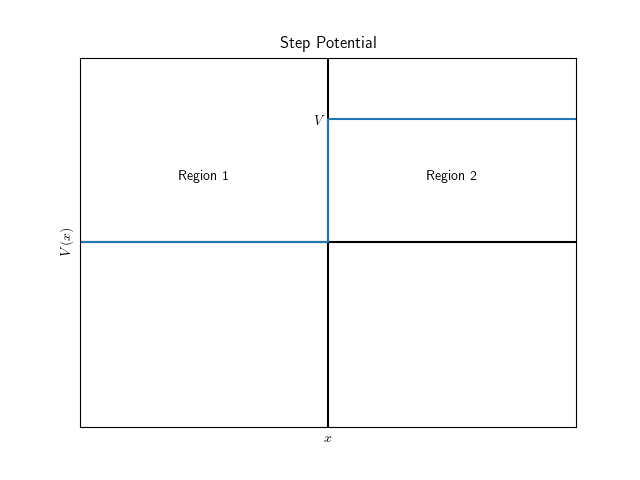
\includegraphics[scale=0.6]{step_potential.png}
        \caption{The step potential}
    \end{figure}
    
    \subsubsection{Case 1: \texorpdfstring{\(E > V\)}{E > V}}
    Classically we would expect a particle incident from the left with \(E > V\) to enter region 2, \(x > 0\).
    Since the total energy of the particle is constant and given by \(H = T + V\) then we would expect that upon entering region 2 the kinetic energy, and hence momentum, of the classical particle will have to decrease to keep the total energy constant.
    
    The \gls{tise} can be split into two section, in region 1, \(x < 0\), we have
    \[-\frac{\hbar^2}{2m}\dv[2]{x}\psi(x) = E\psi(x) \implies \psi''(x) = -\frac{p^2}{\hbar^2}\psi(x)\]
    where
    \[p = \sqrt{2mE},\]
    this is exactly the momentum of a classical particle with energy \(E\) and a potential energy of 0.
    In region 2 we have
    \[\left[-\frac{\hbar^2}{2m}\dv[2]{x}+ V\right]\psi(x) = E\psi(x) \implies \psi''(x) = -\frac{\bar{p}}{\hbar^2}\psi(x)\]
    where
    \[\bar{p} = \sqrt{2m(E - V)},\]
    this is exactly the momentum of a classical particle with energy \(E\) and a potential energy of \(V\).
    As we would expect the momentum in region 2, \(\bar{p}\), is less than the momentum in region 1, \(p\).
    Fortunately we already know the solution to the wave equation in both regions:
    \[
        \psi(x) =
        \begin{cases}
            Ae^{ipx/\hbar} + Be^{-ikp/\hbar}, &x < 0,\\
            Ce^{i\bar{p}x/\hbar} + De^{-i\bar{p}x/\hbar} &x > 0.
        \end{cases}
    \]
    The solutions are a superposition of waves with momentum \(\pm p\) and \(\pm\bar{p}\) in the respective region.
    By `wave with momentum \(p\)' we mean a wave function such that \(p\) is an eigenvalue of \(\operator{P}\).
    
    Suppose that a particle comes in from the left.
    Then we expect a wave propagating to the right in both regions and a wave propagating to the left in region 1 corresponding to the wave reflecting off the boundary.
    However there is no reason to expect a wave propagating left in region 2 as once the wave enters that region there is nothing to cause a reflection.
    Therefore \(D = 0\).
    
    We are left with three degrees of freedom, \(A\), \(B\), and \(C\).
    We can fix one by requiring a normalised wave function, say we choose \(A\) for this purpose.
    We then use the requirements of continuity of \(\psi\) and \(\psi'\) to fix the other two degrees of freedom.
    Clearly \(\psi\) and \(\psi'\) are continuous at all \(x \ne 0\) so we only need to consider continuity at \(x = 0\).
    We require that
    \[\lim_{x\to0^+}\psi(x) = \lim_{x\to0^-}\psi(x),\]
    and
    \[\lim_{x\to0^+}\psi'(x) = \lim_{x\to0^-}\psi'(x).\]
    The first of these gives us
    \[\lim_{x\to0^+}\psi(x) = \lim_{x\to0^+}\left[Ae^{ipx/\hbar} + Be^{-ikx/\hbar}\right] = A + B\]
    \[\lim_{x\to0^-}\psi(x) = \lim_{x\to0^-} Ce^{i\bar{p}x/\hbar} = C.\]
    Hence
    \[A + B = C.\]
    The second leads to 
    \[\lim_{x\to0^+}\psi'(x) = \lim_{x\to0^+}\left[\frac{ip}{\hbar}Ae^{ipx/\hbar} - \frac{ip}{\hbar}Be^{-ikx/\hbar}\right] = \frac{ip}{\hbar}A + \frac{ip}{\hbar}B\]
    \[\lim_{x\to0^-}\psi'(x) = \lim_{x\to0^-} \frac{i\bar{p}}{\hbar}Ce^{i\bar{p}x/\hbar} = \frac{i\bar{p}}{\hbar}C.\]
    Hence
    \[p(A + B) = \bar{p}C.\]
    We can then show that
    \[B = \frac{p - \bar{p}}{p + \bar{p}}A,\qquad\text{and}\qquad C = \frac{2p}{p + \bar{p}}A.\]
    This imposes no restrictions on the energy, \(E\) can take any value as long as it is greater than \(V\).
    The Hamiltonian has a continuous spectrum.
    Notice that in general \(B \ne 0\) so there is a reflected wave going left in region 1.
    
    \subsubsection{Case 2: \texorpdfstring{\(E < V\)}{E<V}}
    The situation is very similar if \(E < V\) but now region 2 is classically forbidden, meaning that a classical particle could not enter into this region.
    The equations for the wave function are the same but since \(E < V\) \(E - V\) is now negative meaning that \(\bar{p}\) is imaginary:
    \[\bar{p} = \sqrt{2m(E - V)} = i\sqrt{2m(V -  E)} = i\tilde{p}.\]
    In region 2 the solution to the wave function is now
    \[\psi(x) = Ce^{-\tilde{p}x/\hbar} + De^{\tilde{p}x/\hbar}.\]
    The first term is a decaying exponential and is finite in region 2.
    The second is an increasing exponential and therefore goes to infinity as \(x \to\infty\).
    This is not allowed so we discard this term in order for \(\psi\) to be normalisable.
    Hence in region 2
    \[\psi(x) = Ce^{-\tilde{p}x/\hbar}.\]
    Region 2 is classically forbidden but the wave function is non-zero in region 2 therefore there is a non-zero probability that the particle will be found in region 2.
    This time we can show that
    \[B = \frac{p - i\tilde{p}}{P + i\tilde{p}}A.\]
    The fraction here has unit modulus so we must have that \(\abs{B}^2 = \abs{A}^2\), this means that they just differ by a phase, \(\delta\):
    \[B = e^{-2i\delta(E)}A,\]
    here we emphasise the fact that \(\delta\) is a function of the energy (not the Dirac delta).
    It can also be shown that
    \[\tilde{p} = p\cot\delta.\]
    We define \(\lambda\) as the length that the particle penetrates the classically forbidden region and we note that it scales as \(\hbar/p\).
    
    \subsection{Potential Barrier}
    Consider the potential
    \[
        V(x) = 
        \begin{cases}
            V, & x \in [0, a],\\
            0, & x\notin[0, a],
        \end{cases}
    \]
    \begin{figure}[ht]
        \centering
        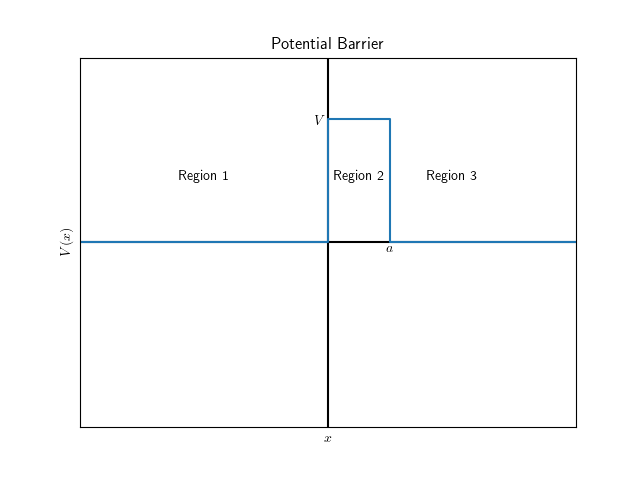
\includegraphics[scale=0.6]{potential_barrier.png}
        \caption{The potential barrier}
    \end{figure}
    for some positive constant, \(V\).
    Again there are two cases, \(E > V\) and \(E < V\).
    In the cases that \(E > V\) this is very similar to the same case with the potential step.
    The wave function will be oscillatory in all three regions with an amplitude that depends on the value of the potential.
    The interesting case is when \(E < V\).
    
    Classically when \(E < V\) region 2 is forbidden.
    A particle entering from the left has no way to go past the origin, it will reflect off the origin and go back to \(-\infty\).
    The solution to the Schr\"odinger equation is
    \[
        \psi(x) =
        \begin{cases}
            Ae^{ipx/\hbar} + Be^{ipx/\hbar}, & x \in (-\infty, 0),\\
            Ce^{-\tilde{p}x/\hbar} + De^{\tilde{p}x/\hbar}, &x \in (0, a),\\
            Fe^{ipx/\hbar} + Ge^{ipx/\hbar}, & x \in (a, \infty).
        \end{cases}
    \]
    Here \(p\) and \(\tilde{p}\) are defined as they were for the potential step.
    Notice that since \(x\) is finite in \((0, a)\) there is no reason to discard the term \(De^{\tilde{p}x/\hbar}\) as it is finite for all \(x\in(0, a)\).
    For the same reason as before if we have a particle coming in from the left we must have that \(G = 0\).
    So in region 3
    \[\psi(x) = Fe^{ipx/\hbar} = AS(E)e^{ip(x - a)/\hbar}.\]
    The last part of this is the conventional way to write this term.
    Of particular interest is \(S(E)\), this is the ratio of the probability amplitude of the wave entering the barrier at \(x = 0\), to the probability amplitude of the wave leaving the barrier at \(x = a\).
    \(S(E)\) can be shown to be
    \[S(E) = \frac{2ip\tilde{p}}{(p^2 - \tilde{p}^2)\sinh(\tilde{p}a/\hbar) + 2ip\tilde{p}\cosh(\tilde{p}a/\hbar)}.\]
    The transmissivity, \(T\), is defined as the probability that the particle tunnels through the barrier, that is
    \[T = \abs{S(E)}^2 = \left[1 + \frac{\sinh^2(\tilde{p}a/\hbar)}{4(E/V)(1 - E/V)}\right]^{-1}.\]
    For \(E < V\) this is a monotonically increasing function of \(E\) for a fixed value of \(a\).
    This means that as the energy increases the probability that the particle tunnels through the barrier increases.
    Importantly
    \[T \propto e^{-ka}\]
    for some constant \(k\).
    Therefore as \(a\) increases for a fixed value of \(E\) the probability that the particle tunnels into region 3 decreases.
    
    \subsubsection{Tunnelling}
    Tunnelling is a phenomenon without classical analogue.
    It can be experimentally verified and is one of many confirmations that quantum mechanics yields correct predictions.
    Tunnelling has many applications in physics.
    
    The process of alpha decay can be seen as a process of the alpha particle tunnelling out of a potential well created by the nucleus.
    Figure~\ref{fig:alpha decay} shows a phenomenological potential used to model alpha decay.
    The alpha particle is in a potential well and typically has less energy than the maximum potential.
    However it is still possible for the alpha particle to tunnel out of the well, and out of the nucleus.
    \begin{figure}[ht]
        \centering
        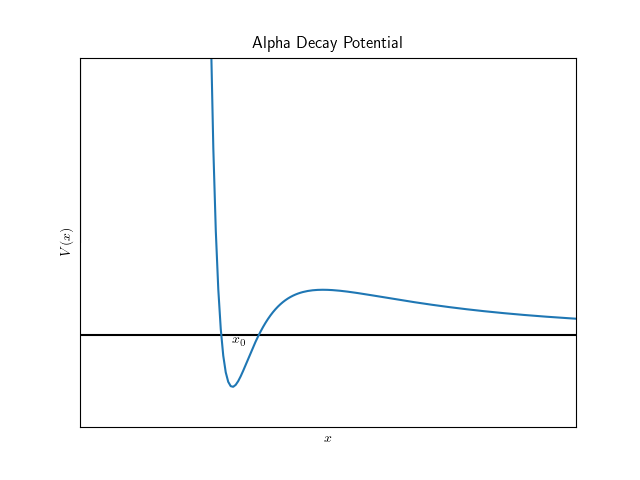
\includegraphics[scale=0.6]{alpha_decay.png}
        \caption{The potential modelling the alpha decay process. An alpha particle in the nucleus is in the potential well at \(x_0\), it can then tunnel outside of this well to some positive \(x\) value even if it has less energy than the peak on the right of the potential well.}
        \label{fig:alpha decay}
    \end{figure}

    \subsubsection{Scanning Tunnelling Microscope}
    A \gls{stm} is made of a needle that is placed near the surface of a material.
    A current of electrons is applied to the needle.
    We can model the air gap between the needle point and the surface as a potential barrier.
    The electrons tunnel across this gap and a current flows.
    The current is proportional to the probability of an electron tunnelling so
    \[I \propto e^{-ka}.\]
    This allows for very small changes in the size of the air gap to be measured accurately by measuring the current.
    Scanning the \gls{stm} over the whole surface we can build up a picture of the 3-dimensional structure of the surface.
    
    \subsection{Infinite Potential Well}\label{sec:infinite square well}
    An infinite potential well of width \(a\) is a potential,
    \[
        V(x) =
        \begin{cases}
            0, & x \in(-a/2, a/2)\\
            \infty, & x\notin (-a/2, a/2).
        \end{cases}
    \]
    We are looking for the solutions to the \gls{tise} with positive energy (as the minimum potential is zero and the energy must be at least as large as this).
    We can view each boundary at \(\pm a/2\) as a potential step and then let \(V\to\infty\).
    The solution in these regions is
    \[\psi \sim e^{-\tilde{p}\delta/\hbar}.\]
    For finite \(V\)
    \[\tilde{p} = \sqrt{2m(V - E)}.\]
    As \(V\to\infty\) \(\tilde{p} \to \infty\) and so \(\psi\to 0\).
    We see that the regions outside of the well are not only classically forbidden but completely inaccessible, even to a quantum particle.
    
    Therefore we only need to solve the \gls{tise} in the region \((-a/2, a/2)\) and apply boundary conditions at \(x = \pm a/2\).
    The boundary conditions here are \(\psi(\pm a/2) = 0\) as we require continuity of \(\psi\).
    Note that since \(V\) is not finite we do not require continuity of \(\psi'\).
    The general form of the solution in the well is that of a free particle:
    \[\psi(x) = Ae^{ikx} + Be^{-ikx}\]
    where \(k = p/\hbar\) and \(p = \sqrt{2mE}\) is the classical momentum.
    At the boundaries we have
    \[\psi(a/2) = Ae^{ika/2} + Be^{-ika/2} = 0 \implies B = -Ae^{ika},\]
    substituting this into the second boundary condition we have
    \begin{align*}
        \psi(-a/2) &= Ae^{-ika/2} - Ae^{ika}e^{ika/2}\\
        &= Ae^{ika/2}(e^{-ika} - e^{ika})\\
        &= Ae^{ika/2}[\cos(ka) - i\sin(ka) - \cos(ka) - i\sin(ka)]\\
        &= 2iAe^{ika/2}\sin(ka).
    \end{align*}
    We require this to be zero.
    Since \(2iAe^{ika/2}\ne 0\) (assuming \(A\) is non-zero, as it must be for any wave function of interest) we must have that \(\sin(ka) = 0\).
    Therefore
    \[ka = n\pi \implies k = \frac{n\pi}{a},\qquad n\in\naturals.\]
    From this we have
    \[\frac{n\pi}{a} = k = \frac{p}{\hbar} = \frac{\sqrt{2mE}}{\hbar} \implies E = \frac{n^2\pi^2\hbar^2}{2ma^2}.\]
    Since \(n\in\naturals\) the energy, \(E\), is quantised.
    From now on we will denote the energy of the \(n\)th state as
    \[E_n = \frac{1}{2m}\left(\frac{\hbar\pi n}{a}\right)^2.\]
    If we normalise the wave functions we find that the properly normalised eigenstates of the Hamiltonian are
    \[
        u_n =
        \begin{cases}
            \sqrt{\frac{2}{a}}\sin\left(\frac{n\pi x}{a}\right), & n~\text{even},\\
            \sqrt{\frac{2}{a}}\cos\left(\frac{n\pi x}{a}\right), & n~\text{odd}.
        \end{cases}
    \]
    Since \(u_n(x) = 0\) is boring we consider \(u_1\) to be the ground state.
    In this state the particle is most likely to be found at \(x = 0\).
    The first four wave functions, and the associated probability densities, are shown in figure~\ref{fig:infinite square well wave functions}.
    \begin{figure}[ht]
        \centering
        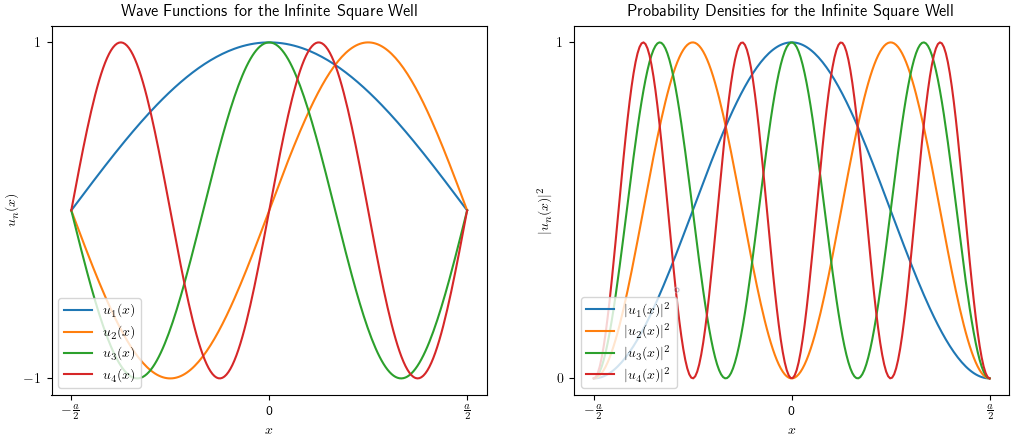
\includegraphics[scale=0.5]{infinite_square_well_wave_func.png}
        \caption{The first four wave functions, \(u_n\), for the infinite square well and the the associated probability densities.}
        \label{fig:infinite square well wave functions}
    \end{figure}
    The generic state of a particle in an infinite square well potential is a linear combination of \(\{u_n(x)\}\).
    That is a linear superposition of eigenstates of \(\operator{P}\) with eigenvalues
    \[\pm p_n = \pm \hbar k_n = \pm\frac{n\pi\hbar}{a}.\]
    
    \subsubsection{Zero Point Energy}
    Notice that in the ground state \(p_1 = \pi\hbar/a \ne 0\).
    This can be seen as a direct consequence of \gls{hup}.
    Since the particle is constrained to have \(x\in(-a/2, a/2)\) this gives us a maximum uncertainty in \(x\) of \(\Delta x = a\).
    Hence
    \[\Delta p\Delta x \ge \frac{\hbar}{2} \implies \Delta p \ge \frac{\hbar}{2a}.\]
    Therefore the momentum cannot be zero, as then we would know the value with zero uncertainty, which is certainly less than \(\hbar/2a\).
    The energy in this state is consequently also non-zero:
    \[E \sim \frac{(\Delta p)^2}{2m} \ge \frac{\hbar^2}{8ma}.\]
    The kinetic energy due to the uncertainty principle is called the zero point energy.
    One consequence of this is that helium can be a liquid at \(T = \SI{0}{\kelvin}\).
    This is because in order to form a solid the atoms must be constrained to a lattice giving them some non-zero zero point energy, which scales inversely to the mass, for a particle as light as helium it is enough to overcome interatomic forces and the system remains in a liquid phase.
    
    \subsubsection{Symmetry of the Solutions}
    The energy eigenstates have definite parity, that is if we define the parity operator, \(\operator{\parity}\), to have the action
    \[\operator{\parity}\psi(x) = \psi(-x),\]
    then the energy eigenstates are also eigenstates of the parity operator:
    \[\operator{\parity}u_n(x) = (-1)^{n+1}u_n(x).\]
    This can be seen from the explicit form of \(u_n\) and using the fact that sine and cosine are odd and even functions respectively.
    This means that \(u_n\) are simultaneously eigenfunctions of \(\operator{\parity}\), \(\operator{P}\), and \(\operator{H}\).
    
    We can show that in general if the potential is symmetric, so \(V(-x) = V(x)\), then \([\operator{H}, \operator{\parity}] = 0\), that is \(\operator{H}\) is symmetric under \(\operator{\parity}\).
    This then implies the existence of a basis of simultaneous eigenstates of \(\operator{H}\) and \(\operator{\parity}\).
    
    It is fairly simple to show the above paragraph is true.
    Suppose that \(V\) is a symmetric potential.
    Then
    \begin{align*}
        \operator{\parity}\operator{H}\psi(x) &= \operator{\parity}\left[-\frac{\hbar^2}{2m}\dv[2]{x} + V(x)\right]\psi(x)\\
        &= \operator{\parity}\left[-\frac{-\hbar^2}{2m}\dv[2]{\psi(x)}{x} + V(x)\psi(x)\right]\\
        &= -\frac{\hbar^2}{2m}\dv[2]{\psi(-x)}{x} + V(-x)\psi(-x)\\
        &= -\frac{\hbar^2}{2m}\dv[2]{\psi(-x)}{x} + V(x)\psi(-x).
     \end{align*}
    Here we have used the fact that
    \[\operator{\parity}\dv{x} = \dv{-x} = -\dv{x}\]
    and hence
    \[\operator{\parity}\dv[2]{x} = -\dv{x}\left(-\dv{x}\right) = \dv[2]{x}.\]
    Also
    \begin{align*}
        \operator{H}\operator{\parity}\psi(x)& = \operator{H}\psi(-x)\\
        &= \left[-\frac{\hbar^2}{2m}\dv[2]{x} + V(x)\right]\psi(-x)\\
        &= -\frac{\hbar^2}{2m}\dv[2]{\psi(-x)}{x} + V(x)\psi(-x).
    \end{align*}
    Hence
    \[[\operator{\parity}, \operator{H}] = 0.\]
    We know that this means there is a common basis of eigenstates but how do we find it?
    The states
    \[v_n^+(x) = u_n(x) + u_n(-x),\qquad\text{and}\qquad v_n^-(x) = u_n(x) - u_n(-x)\]
    are one such basis.
    These states can be compactly written as
    \[v_n^{\pm}(x) = (1 \pm \operator{\parity})u_n(x).\]
    It is then easy to show that these are eigenstates of \(\operator{H}\) and \(\operator{\parity}\):
    \begin{multline*}
        \operator{H}v_n^{\pm}(x) 
        = \operator{H}(1 \pm \operator{\parity})u_n(x) 
        = \operator{H}u_n(x) \pm \operator{H}\operator{\parity}u_n(x) 
        = \operator{H}u_n(x) \pm \operator{\parity}\operator{H}u_n(x) \\
        = E_nu_n(x) + E_n\operator{\parity}u_n(x) 
        = E_n(1 \pm \operator{\parity})u_n 
        = E_nv_n^{\pm}(x).
    \end{multline*}
    and
    \begin{multline*}
        \operator{\parity}v_n^{\pm}(x) 
        = \operator{\parity}(1 \pm \operator{\parity})u_n(x)
        = \operator{\parity}u_n(x) \pm \operator{\parity}^2u_n(x)
        = \operator{\parity}u_n(x) \pm (-1)^{n+1}(-1)^{n+1}u_n(x)\\ 
        = \operator{\parity}u_n(x) \pm u_n(x)
        = \operator{\parity}u_n(x) \pm u_n(x)
        = \pm(1 \pm \operator{\parity})u_n(x)
    \end{multline*}

    \subsection{Finite Potential Well}
    The finite potential well has the potential
    \[
        V(x) = 
        \begin{cases}
            -V_0, & x\int(-a/2, a/2),\\
            0, & x\notin(-a/2, a/2),
        \end{cases}
    \]
    for some positive constant \(V_0\).
    This potential is symmetric under parity change.
    This means that we can look for a set of energy eigenstates that are also parity eigenstates.
    The energy eigenvalues must be greater than \(-V_0\).
    States with \(-V_0 < E < 0\) are called \define{bound states}.
    The wave function for these states decays exponentially for \(\abs{x} > a/2\) so the probability of finding the particle outside of the well becomes small quickly.
    The states with \(E > 0\) are simply plane waves that have a momentum change and chance of reflection at each boundary, this isn't that interesting and is just like the potential step so we won't consider these states further.
    
    The Schr\"odinger equation is
    \[
        \psi''(x) = 
        \begin{cases}
            -\frac{2m}{\hbar^2}E\psi(x), & \abs{x} > a/2,\\
            -\frac{2m}{\hbar^2}(E + V_0)\psi(x), & \abs{x} < a/2.
        \end{cases}
    \]
    Unlike the infinite well the wave function is non-zero outside the well.
    For \(-V_0 < E < 0\) the even parity solutions are
    \[
        \psi(x) =
        \begin{cases}
           A\cos(px/\hbar), & \abs{x} < a/2,\\
           Ce^{-\bar{p}x/\hbar}, & x > a/2,\\
           Ce^{\bar{p}x/\hbar}, & x < -a/2.
        \end{cases}
    \]
    The odd parity solutions are
    \[
        \psi(x) =
        \begin{cases}
            A\sin(px/\hbar), & \abs{x} < a/2,\\
            Ce^{-\bar{p}x/\hbar}, & x > a/2,\\
            -Ce^{\bar{p}x/\hbar}, & x < -a/2.
        \end{cases}
    \]
    We have introduced the momenta
    \[p = \sqrt{2m(E + V_0)},\qquad\text{and}\qquad \bar{p}\sqrt{-2mE}.\]
    There are two things to notice here, first \(-V_0 < E < 0\) so \(p, \bar{p}\in\reals\), and here the factor of \((E + V_0)\) appears in \(p\) whereas previously it appeared in \(\bar{p}\).
    The reason for this is that previously we viewed the minimum of the potential as \(0\) and the maximum as \(V\) but here the minimum is \(-V_0\) and the maximum is \(0\).
    
    Imposing continuity at \(a/2\) in both the wave function and its derivative we have for the even solutions that
    \begin{align*}
        A\cos\left(\frac{pa}{2\hbar}\right) &= Ce^{-\bar{p}a/2\hbar}\\
        -\frac{p}{\hbar}A\sin\left(\frac{pa}{2\hbar}\right) &= -\frac{\bar{p}a}{\hbar}Ce^{-\bar{p}a/2\hbar}.
    \end{align*}
    Dividing the first equation by the second we get the quantisation condition
    \[p\tan\left(\frac{pa}{2\hbar}\right) = \bar{p}.\]
    Similarly for the odd parity solutions we have
    \begin{align*}
        A\sin\left(\frac{pa}{2\hbar}\right) &= Ce^{-\bar{p}a/2\hbar}\\
        \frac{p}{\hbar}A\cos\left(\frac{pa}{2\hbar}\right) &= -\frac{\bar{p}a}{\hbar}Ce^{-\bar{p}a/2\hbar}.
    \end{align*}
    This leads to
    \[p\cot\left(\frac{pa}{2\hbar}\right) = -\bar{p}.\]
    There is always at least one even bound state.
    For small \(V_0\), corresponding to a shallow well, it can be shown that
    \[E = -\frac{mV_0^2a^2}{2\hbar^2}\]
    for the ground state.
    
    \section{Harmonic Oscillators}
    \subsection{The Classical Harmonic Oscillators}
    The equation of motion for a classical particle of mass \(m\) undergoing one-dimensional harmonic oscillations, undergoing a restoring force proportional to the displacement, is
    \[m\ddot{x} = -kx.\]
    The constant \(k\) is often called the spring constant due to the common example of a mass on a spring where this is exactly what \(k\) is.
    The solution is oscillatory with an angular frequency
    \[\omega = \sqrt{\frac{k}{m}}.\]
    Using the chain rule we have
    \[\ddot{x} = \dv[2]{x}{t} = \dv{v}{t} = \dv{v}{x}\dv{x}{t} = v\dv{v}{x}.\]
    Integrating the equation of motion we then have
    \[m\int v\dv{v}{x}\dd{x} = -k\int x\dd{x} \implies \frac{1}{2}mv^2 = -\frac{1}{2}kx^2 + E\]
    where \(E\) is the total energy of the system, which appears as a constant of integration.
    Thus
    \[\frac{1}{2}mv^2 + \frac{1}{2}kx^2 = E.\]
    Identifying the first term as the kinetic energy we see that the potential energy is
    \[V(x) = \frac{1}{2}kx^2 = \frac{1}{2}m\omega^2x^2.\]
    The total energy is
    \[E = \frac{1}{2}m\omega^2L^2\]
    where \(L\) is the amplitude of the oscillations.
    It is easy to show that this is the maximum energy by noting that at \(x = L\) the particle is instantaneously stationary as it changes direction so the kinetic energy is zero.
    
    \subsection{The Quantum Harmonic Oscillator}
    The transformation to the quantum case is straight forward.
    The potential is simply
    \[V(\operator{X}) = \frac{1}{2}m\omega^2\operator{X}^2.\]
    Assuming a discrete spectrum we have to solve the \gls{tise}:
    \[\operator{H}\ket{n} = E_n\ket{n},\]
    where
    \[\operator{H} = \frac{\operator{P}^2}{2m} + \frac{1}{2}m\omega^2\operator{X}^2.\]
    Taking the inner product of the \gls{tise} with an eigenstate of \(\operator{X}\) we have
    \[\bra{x}\operator{H}\ket{n} = E_n\braket{x}{n} = E_nu_n(x)\]
    defining \(u_n(x) = \braket{x}{n}\) as the energy eigenfunction with energy \(E_n\).
    The full \gls{tise} is then
    \[\left[-\frac{\hbar^2}{2m}\dv[2]{x} + \frac{1}{2}m\omega^2 x^2\right]u_n(x) = E_nu_n(x).\]
    
    \subsection{The Solutions to the Harmonic Oscillator}
    We will start by discussing the solutions to this and look at deriving them in later sections.
    The first thing to note is that the energy is quantised as follows:
    \[E_n = \left(n + \frac{1}{2}\right)\hbar\omega,\qquad\text{where}\qquad n\in\naturals.\]
    The ground state corresponds to \(n = 0\) and has the non-zero energy \(E_0 = \hbar\omega/2\).
    The energy eigenfunctions are
    \[u_n(x) = C_ne^{-\alpha^2x^2/2}H_n(\alpha x).\]
    Here \(C_n\) is a normalisation constant, \(\alpha^2 = m\omega/\hbar\) and \(H_n\) are polynomials of degree \(n\) called the \define{Hermite polynomials}.
    The Hermite polynomials are orthogonal in such that
    \[\int_{-\infty}^{\infty} \dd{s}e^{-s^2}H_m(s)H_n(s) = 2^n\sqrt{\pi}n!\delta_{mn},\]
    which is only non-zero if \(n = m\).
    The first four Hermite polynomials are
    \begin{align*}
        H_0(s) &= 1,  & H_2(s) &= 4s^2 - 2,\\
        H_1(x) &= 2s, & H_3(s) &= 8s^3 - 12s.
    \end{align*}
    Note that if \(n\) is even (odd) then \(H_n(s)\) only contains even (odd) powers of \(s\), this is true for all \(n\).
    This means that the Hermite polynomials have even (odd) parity for even (odd) \(n\).
    Since the Gaussian term of \(u_n\) has even parity this means that the parity of \(u_n\) is the same as \(H_n\).
    That is
    \[\operator{\parity}u_n(x) = u_n(-x) = (-1)^nu_n(x).\]
    We see that the energy eigenstates are eigenstates of the parity operator, \(\operator{\parity}\), which is a direct consequence of the potential being symmetric:
    \[V(-x) = \frac{1}{2}m\omega^2(-x)^2 = \frac{1}{2}m\omega^2x^2 = V(x).\]
    Since \(u_n\) has definite parity \(\abs{u_n(x)}^2\) is even.
    Therefore
    \[\expected{x}_n = \bra{n}\operator{X}\ket{n} = \int_{-\infty}^{\infty} \dd{x} x\abs{u_n(x)}^2 = 0,\]
    as the integrand is always odd and an integral of an odd function over an even interval, \((-\infty, \infty)\), is zero.
    Strictly speaking this only holds if the integral converges but in this case it clearly does as the Gaussian part goes to zero much faster than the polynomial parts can go to infinity.
    A quick sanity check here would be to think about the potential and since it is symmetric the particle is equally likely to be at a positive \(x\) as it is at a negative \(x\) and therefore the expected value should be zero.
    
    The next quantity that we might want to compute is the expected value of \(x^2\) which is
    \[\expected{x^2}_n = \int_{-\infty}^{\infty} \dd{x} x^2\abs{u_n(x)}^2 = \left(n + \frac{1}{2}\right)\frac{1}{\alpha^2}.\]
    From this we can see that for larger energies it becomes more probable to find the particle at large \(x\), that is the variance, \(\Delta x_n = \expected{x}_n - \expected{x}_n^2 = \expected{x^2}_n\), increases with energy:
    \[E_n = m\omega^2\expected{x^2}_n.\]
    Compare this to the classical energy,
    \[E = \frac{1}{2}m\omega^2L^2.\]
    
    \subsection{Solving the Harmonic Oscillator (The Fancy Way)}
    \subsubsection{Factorising the Hamiltonian}
    The Hamiltonian is
    \[\operator{H} = \frac{\operator{P}^2}{2m} + \frac{1}{2}m\omega^2\operator{X}^2.\]
    We can factor out \(\hbar\omega\) from this:
    \[\operator{H} = \hbar\omega\left[\frac{1}{2m\hbar\omega}\operator{P}^2 + \frac{m\omega}{2\hbar}\operator{X}^2 \right].\]
    Since \(\hbar\omega\) has units of energy the term in the brackets must be dimensionless.
    We define two operators
    \[\operator{\xi} = \sqrt{\frac{m\omega}{2\hbar}}, \qquad\text{and}\qquad \operator{\eta} = \frac{1}{\sqrt{2m\hbar\omega}}\operator{P}.\]
    These are simply rescaled, dimensionless, versions of the position and momentum operators.
    The Hamiltonian can now be written as
    \[\operator{H} = \hbar\omega[\operator{\xi}^2 + \operator{\eta}^2].\]
    Since \(\operator{\xi}\) and \(\operator{\eta}\) are proportional to the position and momentum operators we know that they don't commute, in fact their commutator is
    \begin{align*}
        [\operator{\xi}, \operator{\eta}] &= \sqrt{\frac{m\omega}{2\hbar}}\frac{1}{\sqrt{2m\hbar\omega}} [\operator{X}, \operator{P}]\\
        &= \frac{1}{2\hbar}[\operator{X}, \operator{P}]\\
        &= \frac{i}{2}.
    \end{align*}
    There are two checks that it is good to do here.
    First since \(\operator{\xi}\) and \(\operator{\eta}\) are dimensionless their commutator should be too, and it is.
    Second since \(\operator{X}\) and \(\operator{P}\) are Hermitian then so are \(\operator{\xi}\) and \(\operator{\eta}\) and therefore their commutator should be anti-Hermitian, and it is.
    
    We now define a new operator:
    \[\operator{a} = \operator{\xi} + i\operator{\eta},\qquad\text{and}\qquad \operator{a}\hermit = \operator{\xi} - i\operator{\eta}.\]
    The motivation behind this is that if \(\operator{\xi}\) and \(\operator{\eta}\) commuted then we could factorise the Hamiltonian as
    \[\hbar\omega(\operator{\xi} + i\operator{\eta})(\operator{\xi} - i\operator{\eta}).\]
    However we cannot do this.
    We can write this new operator in terms of \(\operator{X}\) and \(\operator{P}\):
    \begin{align*}
        \operator{a} &= \sqrt{\frac{m\omega}{2\hbar}} \operator{X} + \frac{i}{\sqrt{2m\omega\hbar}} \operator{P} = \sqrt{\frac{m\omega}{2\hbar}}\left[\operator{X} + \frac{i}{m\omega}\operator{P}\right]\\
        \operator{a}\hermit &= \sqrt{\frac{m\omega}{2\hbar}} \operator{X} - \frac{i}{\sqrt{2m\omega\hbar}} \operator{P} = \sqrt{\frac{m\omega}{2\hbar}}\left[\operator{X} - \frac{i}{m\omega}\operator{P}\right]\\
    \end{align*}
    We can then compute
    \begin{align*}
        \operator{a}\operator{a}\hermit &= (\operator{\xi} + i\operator{\eta})(\operator{\xi} - i\operator{\eta})\\
        &= \operator{\xi}^2 + i\operator{\eta}\operator{\xi} - i\operator{\xi}\operator{\eta} + \operator{\eta}^2\\
        &= \operator{\xi} + i[\operator{\eta}, \operator{\xi}] + \operator{\eta}^2,
    \end{align*}
    and
    \begin{align*}
        \operator{a}\hermit\operator{a} &= (\operator{\xi} - i\operator{\eta})(\operator{\xi} + i\operator{\eta})\\
        &= \operator{\xi}^2 + i\operator{\xi}\operator{\eta} - i\operator{\eta}\operator{\xi} + \operator{\eta}^2\\
        &= \operator{\xi}^2 - i[\operator{\eta}, \operator{\xi}] + \operator{\eta}^2.
    \end{align*}
    Subtracting these two equations we have
    \[[\operator{a}, \operator{a}\hermit] = 1,\]
    and adding the equations we have
    \[\operator{H} = \frac{1}{2}\hbar\omega(\operator{a}\operator{a}\hermit + \operator{a}\hermit\operator{a}).\]
    A more useful form for the Hamiltonian can be found by adding zero:
    \[\operator{H} = \frac{1}{2}\hbar\omega(\operator{a}\operator{a}\hermit + \operator{a}\hermit\operator{a}) = \frac{1}{2}\hbar\omega(\operator{a}\operator{a}\hermit - \operator{a}\hermit\operator{a} + \operator{a}\hermit\operator{a}+ \operator{a}\hermit\operator{a}) = \frac{1}{2}\hbar\omega([\operator{a}, \operator{a}\hermit] + 2\operator{a}\hermit\operator{a}) = \hbar\omega\left(\operator{a}\hermit\operator{a} + \frac{1}{2}\right).\]
    
    \subsubsection{Creation and Annihilation}
    For this section we will need the commutators of \(\operator{a}\) and \(\operator{a}\hermit\) with the Hamiltonian, fortunately these are fairly easy to compute now:
    \[[\operator{H}, \operator{a}] = \left[\hbar\omega\left(\operator{a}\hermit \operator{a} + \frac{1}{2}\right), \operator{a}\right] = \hbar\omega[\operator{a}\hermit\operator{a}, \operator{a}]\]
    using the fact that \([1/2, \operator{a}] = 0\).
    Then
    \[[\operator{a}\hermit\operator{a}, \operator{a}] = \operator{\hermit}\operator{a}\operator{a} - \operator{a}\operator{a}\hermit\operator{a} = [\operator{a}\hermit, \operator{a}]\operator{a} = -\operator{a}.\]
    Therefore
    \[[\operator{H}, \operator{a}] = \hbar\omega [\operator{a}\hermit\operator{a}, \operator{a}] = -\hbar\omega\operator{a.}\]
    Similarly
    \[[\operator{H}, \operator{a}\hermit] = \left[\hbar\omega\left(\operator{a}\hermit \operator{a} + \frac{1}{2}\right), \operator{a}\hermit\right] = \hbar\omega[\operator{a}\hermit\operator{a}, \operator{a}\hermit] = \hbar\omega(\operator{a}\hermit\operator{a}\operator{a}\hermit - \operator{a}\hermit\operator{a}\hermit\operator{a}) = \hbar\omega\operator{a}\hermit[\operator{a}, \operator{a}\hermit] = \hbar\omega\operator{a}\hermit.\]
    Suppose \(\ket{n}\) is an energy eigenstate.
    We would like to know how \(\operator{a}\) acts on this since working in the energy eigenbasis we can then describe the action of \(\operator{a}\) on any state.
    To do this we will use that
    \[\operator{H}\operator{a} = \operator{a}\operator{H} + \operator{H}\operator{a} - \operator{a}\operator{H} = \operator{a}\operator{H} + [\operator{H}, \operator{a}].\]
    Thus
    \begin{align*}
        \operator{H}(\operator{a}\ket{n}) &= \operator{a}\operator{H}\ket{n} + [\operator{H}, \operator{a}]\ket{n}\\
        &= E_n\operator{a}\ket{n} - \hbar\omega\operator{a}\ket{n}\\
        &= (E_n - \hbar\omega)\operator{a}\ket{n}.
    \end{align*}
    So we see that \(\operator{a}\ket{n}\) is another eigenstate of \(\operator{H}\) with energy \(E_n - \hbar\omega\), unless \(\operator{a}\ket{n} = 0\).
    For this reason we say that \(\operator{a}\) is a \define{lowering operator} as its action is to return an eigenstate of lower energy.
    It is also called an \define{annihilation operator} as it annihilates one quantum of energy, \(\hbar\omega\), from the system.\footnote{\(\operator{a}\) and \(\operator{a}\hermit\) don't correspond to physical processes so we don't need to consider energy conservation.}
    Similarly
    \begin{align*}
        \operator{H}(\operator{a}\dagger\ket{n}) &= \operator{a}\operator{H}\ket{n} + [\operator{H}, \operator{a}\hermit]\\
        &= E_n\operator{a}\ket{n} + \hbar\omega\operator{a}\hermit\\
        &= (E_n + \hbar\omega)\operator{a}\hermit\ket{n}.
    \end{align*}
    So again \(\operator{a}\hermit\ket{n}\) is an energy eigenstate, this time with higher energy \(E_n + \hbar\omega\).
    We call \(\operator{a}\hermit\) a \define{raising operator} as its action is to return an eigenstate of higher energy.
    It is also called a \define{creation operator} as it adds one quantum of energy, \(\hbar\omega\), to the system.
    
    If \(\ket{n}\) is an energy eigenstate with energy \(E_n\) then define \(\ket{n\pm 1}\) to be an energy eigenstate with energy \(E_n \pm \hbar\omega\).
    Then
    \[\operator{a}\ket{n} = c_n\ket{n - 1},\qquad\text{and}\qquad \operator{a}\hermit\ket{n} = d_n\ket{n + 1}.\]
    Here \(c_n\) and \(d_n\) are constants of proportionality and not eigenvalues.
    
    By successive application of the annihilation operator, \(\operator{a}\), we can get states with lower and lower energy unless at some point \(\operator{a}\ket{0} = 0\) we call the state \(\ket{0}\) the ground state.
    Such a state must exist as the potential is bounded below and the energy is always at least as large as the minimum of the potential.
    We can find the ground state energy by applying the Hamiltonian:
    \[\operator{H}\ket{0} = \hbar\omega \left(\operator{a}\hermit\operator{a} + \frac{1}{2}\right)\ket{0} =  \hbar\omega\operator{a}\hermit\underbrace{\operator{a}\ket{0}}_{=0}\frac{\hbar\omega}{2}\ket{0} = \frac{\hbar\omega}{2}\ket{0}\]
    so we see that the ground state of the Harmonic oscillator has energy \(\hbar\omega/2\).
    
    Going the other way we can start from the ground state and construct states with progressively higher and higher energies by applying the creation operator, \(\operator{a}\hermit\).
    Unlike with the annihilation operator there is no reason that this should ever yield zero as the energy is in theory unbounded above.
    The first application of the creation operator gives
    \[\operator{a}\hermit \ket{0} = d_0\ket{1}\]
    where \(\ket{1}\) is a state with energy
    \[E_1 = \hbar\omega\left(1 + \frac{1}{2}\right) = \frac{3}{2}\hbar\omega.\]
    A second application gives
    \[\operator{a}\hermit{^2}\ket{0} = d_0\operator{a}\hermit\ket{1} = d_0d_1\ket{2}.\]
    At this point we see that we really need to know what \(c_n\) and \(d_n\) are.
    We find them by considering the expectation values of \(\operator{a}\hermit\operator{a}\) and \(\operator{a}\operator{a}\hermit\) and requiring all states be normalised:
    \begin{align*}
        \bra{n}\operator{a}\hermit\operator{a}\ket{n} &= c_n\bra{n}\operator{a}\hermit\ket{n - 1}\\
        &= c_n\bra{n-1}\operator{a}\ket{n}^*\\
        &= c_nc_n^*\braket{n-1}{n-1}\\
        &= \abs{c_n}^2.
    \end{align*}
    Also
    \[\operator{a}\hermit\operator{a} = \frac{1}{\hbar\omega}\operator{H} - \frac{1}{2}\]
    so
    \begin{align*}
        \bra{n}\operator{a}\hermit\operator{a}\ket{n} &= \frac{1}{\hbar\omega}\bra{n}\operator{H}\ket{n} - \frac{1}{2}\braket{n}{n}\\
        &= \frac{1}{\hbar\omega}E_n\braket{n}{n} - \frac{1}{2}\braket{n}{n}\\
        &= \frac{1}{\hbar\omega}\left(n + \frac{1}{2}\right)\hbar\omega  - \frac{1}{2}\\
        &= n
    \end{align*}
    Since states are only defined up to a phase factor we are free to choose \(c_n\) to be a real, positive, number so
    \[c_n = \sqrt{n}.\]
    For \(d_n\) consider
    \begin{align*}
        \bra{n}\operator{a}\operator{a}\hermit\ket{n} &= d_n \bra{n}\operator{a}\ket{n + 1}\\
        &= d_n\bra{n + 1}\operator{a}\hermit\ket{n}^*\\
        &= d_nd_n^*\braket{n + 1}{n + 1}
    \end{align*}
    Also
    \[\operator{a}\operator{a}\hermit = \frac{1}{\hbar\omega}\operator{H} + \frac{1}{2}\]
    so
    \begin{align*}
        \bra{n}\operator{a}\operator{a}\hermit\ket{n} &= \frac{1}{\hbar\omega}\bra{n}\operator{H}\ket{n} + \frac{1}{2}\braket{n}{n}\\
        &= \frac{1}{\hbar\omega}E_n\braket{n}{n} + \frac{1}{2}\braket{n}{n}\\
        &= \frac{1}{\hbar\omega}\left(n + \frac{1}{2}\right)\hbar\omega + \frac{1}{2}\\
        &= n + 1.
    \end{align*}
    So, again choosing \(d_n\) to be real and positive, we have
    \[d_n = \sqrt{n + 1}.\]
    So the full action of the raising and lowering operators is
    \[\operator{a}\ket{n} = \sqrt{n}\ket{n - 1},\qquad\text{and}\qquad \operator{a}\hermit\ket{n} = \sqrt{n + 1}\ket{n + 1}.\]
    We see that the action of \(\operator{a}\) on the ground state is
    \[\bra{x}\operator{a}\ket{0} = \bra{x}\sqrt{0}\ket{?} = 0\]
    for all \(\ket{x}\), as expected.
    
    \subsubsection{The Wave Function}
    We have introduced these creation and annihilation operators but we have yet to show that they allow us to find the correct wave functions for the system.
    We define \(\braket{x}{n} = u_n(x)\) and also we know for the ground state that \(\bra{x}\operator{a}\ket{0} = \operator{a}u_0(x) = 0\).
    We can also expand this with the definition of \(\operator{a}\) in terms of position and momentum operators:
    \begin{align*}
        0 &= \operator{a}u_0(x)\\
        &= \sqrt{\frac{m\omega}{2\hbar}}\left[\operator{X} + \frac{i}{m\omega}\operator{P}\right]u_0(x)\\
        &= \sqrt{\frac{m\omega}{2\hbar}}\left[x - \frac{i}{m\omega}i\hbar\dv{x}\right]u_0(x)\\
        \implies 0 &= xu_0(x) + \frac{\hbar}{m\omega}\dv{u_0}{x}\\
        \implies \dv{u_0}{x} &= -\frac{m\omega}{\hbar}xu_0(x)\\
        &= \alpha^2xu_0(x)\\
        \implies \frac{1}{u_0}\dv{u_0}{x} &= -\alpha x\\
        \implies \int \frac{1}{u_0}\dd{u_0} &= -\alpha^2 \int x \dd{x}\\
        \implies \ln(u_0) &= -\frac{1}{2}\alpha^2x^2 + \ln(N)
        \shortintertext{where \(\ln C\) is a constant of integration}
        \implies u_0 &= Ce^{-\alpha^2 x^2/2}.
    \end{align*}
    We can find \(C\) by requiring the state to be normalised so
    \begin{align*}
        1 &= \int_{-\infty}^{\infty} \abs{u_0(x)}^2 \dd{x}\\
        &= C^2 \int_{-\infty}^{\infty} e^{-\alpha^2x^2}\\
        &= C^2 \frac{\sqrt{\pi}}{\alpha}\\
        \implies C &= \frac{\sqrt{\alpha}}{\pi^{1/4}}.
    \end{align*}
    where we have used the standard result
    \[\int_{-\infty}^{\infty} e^{-p(x + q)^2} \dd{x} = \sqrt{\frac{\pi}{p}}.\]
    
    We can then construct any wave function by successive applications of \(\operator{a}\hermit\).
    However we must account for the constants of proportionality, for example
    \[\operator{a}\hermit{^4}\ket{0} = \sqrt{1}\operator{a}\hermit{^3}\ket{1} = \sqrt{1}\sqrt{2}\operator{a}\hermit{^2}\ket{2} = \sqrt{1}\sqrt{2}\sqrt{3}\operator{a}\hermit\ket{3} = \sqrt{1}\sqrt{2}\sqrt{3}\sqrt{4}\ket{4} = \sqrt{4!}\ket{4}.\]
    In general
    \[\ket{n} = \frac{1}{\sqrt{n!}}\operator{a}\hermit{^n}\ket{0}.\]
    Note that these states may still not be normalised as \(\operator{a}\hermit\) is not Hermitian so there is no guarantee that it preserves inner products.
    In terms of wave functions then we have
    \begin{align*}
        u_n(x) &= \frac{1}{\sqrt{n!}}\operator{a}\hermit{^n}u_0(x)\\
        &= \frac{1}{\sqrt{n!}}\left[\sqrt{\frac{m\omega}{2\hbar}} \left(\operator{X} - \frac{i}{m\omega}\operator{P}\right)\right]^nu_0(x)\\
        &= \frac{1}{\sqrt{n!}}\left[\sqrt{\frac{m\omega}{2\hbar}} \left(x - \frac{\hbar}{m\omega}\dv{x}\right)\right]^nu_0(x)\\
    \end{align*}
    Computing this we will recover the Hermite polynomials.
    
    \section{Systems in Three Spatial Dimensions}
    \subsection{States}
    As with the one-dimensional case the state is described by a state vector, \(\ket{\psi}\in\hilbert\).
    The position eigenbasis is now represented by position vectors, \(\vv{r}\), so the basis is \(\{\ket{\vv{r}}\}\).
    A generic state vector is then
    \[\ket{\psi} = \int\dd[3]{r}\bra{\vv{r}}\braket{\vv{r}}{\psi} = \int \dd[3]{r} \psi(\vv{r})\ket{\vv{r}}\]
    where
    \[\psi(\vv{r}) = \braket{\vv{r}}{\psi}.\]
    The probability density is given by \(\abs{\psi(\vv{r})}^2\) and \(\abs{\psi(\vv{r})}^2\dd[3]{r}\) then gives the probability that the particle is found in the volume element \(\dd[3]{r}\) at position \(\vv{r}\).
    Introducing some time dependence a generic state becomes
    \[\ket{\Psi(t)} = \int \dd[3]{r} \ket{\vv{r}}\braket{\vv{r}}{\Psi(t)} = \int \dd[3]{r} \Psi(\vv{r}, t)\ket{\vv{r}},\]
    where
    \[\Psi(\vv{r}, t) = \braket{\vv{r}}{\Psi(t)}.\]
    An inner product between two states, \(\ket{\Psi(t)}, \ket{\Phi(t)}\in\hilbert\) is 
    \[\braket{\Phi(t)}{\Psi(t)} = \int \dd[3]{r} \Phi^*(\vv{r}, t)\Psi(\vv{r}, t).\]
    As usual we require normalised states so
    \[\braket{\Psi(t)}{\Psi(t)} = \int_{\text{all space}} \dd[3]{r}\abs{\Psi(t)}^2 = 1.\]
    
    The only change so far from the one-dimensional case is that \(x\) becomes \(\vv{r}\) and \(\dd{x}\) becomes \(\dd[3]{r}\).
    
    \subsection{Observables}
    An observable, \(O\), is still associated with a Hermitian operator, \(\operator{O}\colon\hilbert\to\hilbert\) which we can think of as acting on the wave function with the usual identification that
    \[\operator{O}\ket{\psi} = \bra{\vv{r}}\operator{O}\ket{\psi}.\]
    The eigenvalue equation is still
    \[\operator{O}\psi_k(\vv{r}) = O_k\psi_k(\vv{r})\]
    where \(\{\psi_k\}\) are the eigenfunctions of \(\operator{O}\).
    Again \(\{\ket{\psi_k}\}\) form a basis for \(\hilbert\).
    The eigenvalues, \(\{O_k\}\), are all possible outcomes of the measurement and the specific eigenvalue \(O_k\), when measuring \(O\) in state \(\ket{\psi}\in\hilbert\), occurs with probability
    \[\abs{c_k}^2 = \abs{\braket{\psi_k}{\psi}}^2.\]
    The Hermitian conjugate is still defined as
    \[\bra{\varphi}\operator{O}\hermit\ket{\psi} = \bra{\psi}\operator{O}\ket{\varphi}^*,\]
    or in terms of wave functions
    \[\int \dd[3]{r} \varphi^*(\vv{r})\operator{O}\hermit \psi(\vv{r}) = \left[\int \dd[3]{r} \psi^*(\vv{r}) \operator{o} \varphi(\vv{r})\right]^*.\]
    
    \subsubsection{Position Operator}
    The three-dimensional position operator is a vector of one-dimensional position operators:
    \[\vecoperator{X} = (\operator{X}, \operator{Y}, \operator{Z}) = (\operator{X}_1, \operator{X}_2, \operator{X}_3).\]
    Which have the expected application of multiplication by their respective Cartesian coordinate:
    \[\operator{X}_k \psi(\vv{r}) = x_k\psi(\vv{r})\]
    where \(\vv{r} = (x_1, x_2, x_3)\).
    
    \subsubsection{Momentum Operator}
    The three-dimensional momentum operator is a vector of one-dimensional momentum operators:
    \[\vecoperator{P} = (\operator{P}_x, \operator{P}_y, \operator{P}_z) = (\operator{P}_1, \operator{P}_2, \operator{P}_3).\]
    Each one-dimensional operator is
    \[\operator{P}_k = -i\hbar\pdv{x_k} = -i\hbar\partial_k,\]
    which when applied to a wave function gives
    \[\operator{P}_k\psi(\vv{r}) = -i\hbar\pdvat{\psi}{x_i}{\vv{r}}.\]
    We can concisely write the momentum operator with some vector calculus notation as
    \[\vecoperator{P} = -i\hbar\grad\]
    where \(\grad = (\partial_1, \partial_2, \partial_3)\) is the gradient operator.
    
    \subsubsection{The Canonical Commutation Relation}
    The partial derivatives commute so
    \[\operator{P}_i\operator{P}_j\psi(\vv{r}) = -\hbar^2\pdvsec{\psi}{x_i}{x_j} = -\hbar^2\pdvsec{\psi}{x_j}{x_i} = \operator{P}_j\operator{P}_i\psi(\vv{r}).\]
    This means that
    \[[\operator{P}_i, \operator{P}_j] = 0.\]
    Clearly \(x_ix_j = x_jx_i\) so
    \[[\operator{X}_i, \operator{X}_j] = 0.\]
    More interestingly we can look at \([\operator{X}_i, \operator{P}_j]\).
    We know that in the case \(i = j\) this is the same as the one-dimensional canonical commutation relation and therefore equal to \(i\hbar\).
    In general
    \[\operator{X}_i\operator{P}_j\psi = -i\hbar\operator{X_i}\pdv{\psi}{x_j} = -i\hbar x_i\pdv{\psi}{x_j}\]
    and
    \[\operator{P}_j\operator{X}_i\psi = \operator{P}_j[x_i\psi] = -i\hbar\pdv{x_i}{x_j} - i\hbar x_i\pdv{\psi}{x_j} = \operator{P}_j[x_i\psi] = -i\hbar\delta_{ij} - i\hbar x_i\pdv{\psi}{x_j}.\]
    Therefore
    \[[\operator{X}_i, \operator{P}_j] = -i\hbar x_i\pdv{\psi}{x_j} + i\hbar\delta_{ij} + i\hbar x_i\pdv{\psi}{x_j} = i\hbar\delta_{ij}.\]
    In the case that \(i = j\) we have that \(\delta_{ij} = 1\) and so this reduces to the expected relation in one-dimension.
    
    Since orthogonal position and momentum operators commute there is no need for them to follow the \gls{hup}, however parallel position and momentum operators must still follow the \gls{hup}, thus
    \[\Delta x_i\Delta p_j \ge \frac{\hbar}{2}\delta_{ij}.\]
    
    \subsection{Dynamics}
    The dynamics of the three-dimensional system are still given by the Schr\"odinger equation,
    \[\operator{H}\ket{\Psi(t)} = i\hbar\dv{t}\ket{\Psi(t)},\]
    where
    \[\operator{H} = \frac{\vecoperator{P}\cdot\vecoperator{P}}{2m} + V(\vecoperator{X}).\]
    The action of this one a wave function is then
    \[\operator{H} = \frac{-\hbar^2}{2m}\laplacian + V(\vv{r}).\]
    The \gls{tise} is still
    \[\operator{H}\ket{\psi} = E\ket{\psi}\]
    and the time evolution operator is still
    \[\operator{U}(t) = e^{-i\operator{H}t/\hbar}.\]
    
    \subsubsection{Three-Dimensional Harmonic Oscillator}
    The three-dimensional isotropic harmonic oscillator has the same potential
    \[V(\vv{r}) = \frac{1}{2}m\omega^2r^2 = \frac{1}{2}m\omega^2(x^2 + y^2 + z^2).\]
    We can separate the \gls{tise} into a product of three terms,
    \[\psi(\vv{r}) = X(x)Y(y)Z(z),\]
    which each depend on only one coordinate.
    Using this the \gls{tise} becomes
    \begin{align*}
        EX(x)Y(y)Z(z) &= \left[-\frac{\hbar^2}{2m}\laplacian + \frac{1}{2}m\omega^2(x^2 + y^2 + z^2)\right]X(x)Y(y)Z(z)\\
        &= -\frac{\hbar^2}{2m}\left(\dv[2]{X}{x}Y(y)Z(z) + X(x)\dv[2]{Y}{y}Z(z) + X(x)Y(y)\dv[2]{Z}{z}\right) \\
        &\qquad+ \frac{1}{2}m\omega^2(x^2 + y^2 + z^2)X(x)Y(y)Z(z)
    \end{align*}
    Since the three terms \(X\), \(Y\), and \(Z\) only depend on one coordinate and therefore their derivatives with respect to any other coordinate are zero.
    Dividing through by \(X(x)Y(y)Z(z)\) and factorising we have
    \[E = \left[-\frac{\hbar^2}{2m}\dv[2]{X}{x}\frac{1}{X} + \frac{1}{2}m\omega^2x^2\right] + \left[-\frac{\hbar^2}{2m}\dv[2]{Y}{y}\frac{1}{Y} + \frac{1}{2}m\omega^2y^2\right] + \left[-\frac{\hbar^2}{2m}\dv[2]{Z}{z}\frac{1}{Z} + \frac{1}{2}m\omega^2z^2\right].\]
    The left hand side is a constant, each term in brackets depends on only one coordinate, and we can vary two coordinates without varying the third.
    This means that each term in brackets must be constant so
    \[E_{n_x} + E_{n_y} + E_{n_z} = E\]
    where
    \[E_{n_x} = \left[-\frac{\hbar^2}{2m}\dv[2]{X}{x}\frac{1}{X} + \frac{1}{2}m\omega^2x^2\right],\]
    and \(E_{n_y}\) and \(E_{n_z}\) are similarly defined.
    We can identify each term as a Harmonic oscillator in one dimension and we already know the solutions for these.
    The energy corresponding to the \(x\) direction is then
    \[E_{n_x} = \left(n_x + \frac{1}{2}\right)\hbar\omega.\]
    The solution in the \(x\) direction is
    \[X(x) = u_{n_x}(x) = C_{n_(x)}e^{-\alpha^2x^2/2}H_{n_x}(\alpha x).\]
    The same can be done for the \(y\) and \(z\) directions.
    The energy eigenvalue for the whole system is then
    \[E_n = \left(n_x + n_y + n_z + \frac{3}{2}\right)\hbar\omega = \left(n + \frac{3}{2}\right)\hbar\omega.\]
    The solution to the whole system is
    \[\psi_{n_x,n_y,n_z}(\vv{r}) = u_{n_x}(x)u_{n_y}(y)u_{n_z}(z).\]
    
    One new thing that we didn't have in the one-dimensional case is degeneracy.
    Suppose the total energy is \(5\hbar\omega/2\).
    That is \(n = 1\).
    Then there are three ways to have this happen, any one of \(n_x\), \(n_y\), and \(n_z\) could be one and the other two will be zero.
    We say that \(E_n\) is three-fold degenerate.
    Table~\ref{tab:degeneracy 3D HO} shows different ways that the same energy eigenvalue, \(E_n\), can be degenerate for \(n = 0, 1, 2\).
    Clearly these grow quite quickly.
    With some basic combinatorics we can find a general statement for the degeneracy of the \(n\)th energy eigenvalue.
    First choose \(n_x\) to be some integer such that \(0 \le n_x \le n\).
    Then \(n_y + n_z = n - n_x\) so pick \(n_y\) to be some integer such that \(0 \le n_y \le n - n_x\).
    Finally choose \(n_z\) such that \(n_x + n_y + n_z = n\).
    There are \(n + 1\) ways to choose \(n_x\) and then for each of these choices there are \(n - n_x + 1\) ways to choose \(n_y\) and then \(n_z\) is fixed by these choices.
    Thus
    \begin{align*}
        g_n &= \sum_{n_x = 0}^{n+1}(n - n_x + 1)\\
        &= \sum_{n_x = 0}^{n+1}(n + 1) - \sum_{n_x = 0}^{n+1}n_x\\
        &= (n+1)(n+1) - \frac{1}{2}(n+1)(n+2)\\
        &= (n+1)\left[(n+2) - \frac{1}{2}(n+2)\right]\\
        &= \frac{1}{2}(n+1)(n+2)
    \end{align*}
    Where we have used the result that
    \[\sum_{k=0}^{N}k = \frac{1}{2}N(N + 1)\]
    which can be readily proven by induction, as we have done in appendix~\ref{sec:proof sum 0 to n of r is 0.5 n(n+1)}.
    \begin{table}
        \centering
        \begin{tabular}{ccccc}
        	\hline\hline
        	\(n\) & \(n_x\) & \(n_y\) & \(n_z\) & \(g_n\) \\\hline\hline
        	  0   &    0    &    0    &    0    &    1\\\hline
                  &    1    &    0    &    0    &\\
              1   &    0    &    1    &    0    &    3\\
                  &    0    &    0    &    1    &\\\hline
                  &    2    &    0    &    0    &\\
                  &    0    &    2    &    0    &\\
              2   &    0    &    0    &    2    &    6\\
                  &    1    &    1    &    0    &\\
                  &    1    &    0    &    1    &\\
                  &    0    &    1    &    1    &\\\hline\hline
        \end{tabular}
        \caption{Demonstrating the degeneracy of the \(E_n\) energy eigenvalue, for \(n = 0, 1, 2\), for the three-dimensional harmonic oscillator.}
        \label{tab:degeneracy 3D HO}
    \end{table}

    \endgroup
    
    
    \part{Angular Momentum and Spin}
    \section{Angular Momentum}
    \subsection{Angular Momentum in Classical Mechanics}
    In classical mechanics the angular momentum of a particle at position \(\vv{x}\) with momentum \(\vv{p}\) is
    \[\vv{L} = \vv{x} \times \vv{p}.\]
    As a vector equation this can be written as three scalar equations:
    \[L_x = yp_z - zp_y, \qquad L_y = zp_x - xp_z,\qquad\text{and}\qquad L_z = xp_y - yp_x.\]
    These can be written more concisely as
    \[L_i = \varepsilon_{ijk}x_jp_k\]
    where \((x_1, x_2, x_3) = (x, y, z)\) and \((p_1, p_2, p_3) = (p_x, p_y, p_z)\) and \(\varepsilon_{ijk}\) is the Levi-Civita symbol defined as
    \[
        \varepsilon_{ijk} = 
        \begin{cases}
            1, & (i,j,k) = (1, 2, 3), (2, 3, 1), (3, 1, 2),\\
            -1, & (i, j, k) = (1, 3, 2), (2, 1, 3), (3, 2, 1),\\
            0, & \text{otherwise},
        \end{cases}
    \]
    and we have applied the Einstein summation convention of summing over repeated indices.
    
    \subsection{Angular Momentum in Quantum Mechanics}
    \subsubsection{Angular Momentum Operators}
    Angular momentum is an observable and so has an associated Hermitian operator.
    The \define{angular momentum operator} for the angular momentum in the \(\ve{i}\) direction is
    \[\operator{L}_i = \varepsilon_{ijk}\operator{X}_j\operator{P}_k.\]
    We can write this as a cross product of vectors of operators:
    \[\vecoperator{L} = \vecoperator{X}\times\vecoperator{P}.\]
    For a state \(\ket{\psi}\in\hilbert\) if we define \(\operator{L}_k\ket{\psi} = \ket{\varphi}\) then
    \[\bra{\vv{r}}\operator{L}_k\ket{\psi} = \braket{\vv{r}}{\varphi} = \varphi(\vv{r}) = \operator{L}_k\psi(\vv{r}) = -\hbar\varepsilon_{ijk}x_j\pdv{\psi}{x_k}.\]
    
    \subsubsection{Angular Momentum Commutators}
    Since \(\operator{L}_i\) are defined as a product of position and momentum operators we expect the commutation relations between different components of the angular momentum to be non-trivial, for example:
    \begin{align*}
        [\operator{L}_x, \operator{L}_y] &= [\operator{Y}\operator{P}_z - \operator{Z}\operator{P}_y, \operator{Z}\operator{P}_x - \operator{X}\operator{P_z}]\\
        &= [\operator{Y}\operator{P}_z, \operator{Z}\operator{P}_x] - [\operator{Z}\operator{P}_y, \operator{Z}\operator{P_x}] - [\operator{Y}\operator{P}_z, \operator{X}\operator{P}_z] + [\operator{Z}\operator{P}_y, \operator{X}\operator{P}_z]\\
        &= [\operator{Y}\operator{P}_z, \operator{Z}\operator{P}_x] - \operator{Z}[\operator{P}_y, \operator{P}_x] - [\operator{Y}, \operator{X}]\operator{P}_z + [\operator{Z}\operator{P}_y, \operator{X}\operator{P}_z]\\
        &= \operator{Y}\operator{P}_z\operator{Z}\operator{P_x} - \operator{Z}\operator{P}_x\operator{Y}\operator{P}_z + \operator{Z}\operator{P}_y\operator{X}\operator{P_z} - \operator{X}\operator{P}_z\operator{Z}\operator{P}_y\\
        &= \operator{Y}\operator{P}_x(\operator{P}_z\operator{Z} - \operator{Z}\operator{P}_z) + \operator{X}\operator{P}_y(\operator{Z}\operator{P}_z - \operator{P}_z\operator{Z})\\
        &= \operator{Y}\operator{P}_x[\operator{P}_z, \operator{Z}] + \operator{X}\operator{P}_y[\operator{Z}, \operator{P}_z]\\
        &= -i\hbar\operator{Y}\operator{P}_x + i\hbar\operator{X}\operator{P}_y\\
        &= i\hbar\operator{L}_z.
    \end{align*}
    A couple of sanity checks that we can perform here are that \(\operator{L}_k\) is Hermitian so the commutator should be anti-Hermitian, which it is, and also the units of the commutator are angular momentum squared and \(\hbar\) and \(\operator{L}_z\) also both have units of angular momentum so the units match.
    Noting that \([\operator{L}_i, \operator{L}_j] = -[\operator{L}_j, \operator{L}_i]\) and \([\operator{L}_i, \operator{L}_i] = 0\) we have that
    \[[\operator{L}_i, \operator{L}_j] = i\hbar\varepsilon_{ijk}\operator{L}_k.\]
    Since this is non-zero when \(i\ne j\) we see that measuring the angular moment in one direction and then another changes the probability for measuring the angular momentum in the first direction.
    
    \subsubsection{Angular Momentum Differential Operators}
    As with the other operators we have introduced we can view \(\operator{L}_i\) as differential operators acting on the wave function.
    In this case
    \[\operator{L}_x = \varepsilon_{1jk}\operator{X}_j\operator{P}_k = \operator{X}_2\operator{P}_3 - \operator{X}_3\operator{P}_2 = -i\hbar\left(y\pdv{z} - z\pdv{y}\right).\]
    Similarly
    \[\operator{L}_y = -i\hbar\left(z\pdv{x} - x\pdv{z}\right), \qquad\text{and}\qquad \operator{L}_z = -i\hbar\left(x\pdv{y} - y\pdv{x}\right).\]
    Or more compactly
    \[\operator{L}_i = -i\hbar\varepsilon_{ijk}x_j\pdv{x_k}.\]
    We can use these to derive the commutation relationships that we derived in the last section using the canonical commutation relationship:
    \begin{align*}
        \operator{L}_x\operator{L}_y\psi &= -\hbar^2\left(y\pdv{z} - z\pdv{y}\right)\left(z\pdv{x} - x\pdv{z}\right)\psi\\
        &= -\hbar^2\left(y\pdv{z} - z\pdv{y}\right) \left(z\pdv{\psi}{x} - x\pdv{\psi}{z}\right)\\
        &= -\hbar^2\left[y\pdv{z}\left(z\pdv{\psi}{x}\right) - y\pdv{z}\left(x\pdv{\psi}{z}\right) - z\pdv{y}\left(z\pdv{\psi}{x}\right) + z\pdv{y}\left(x\pdv{\psi}{z}\right)\right]\\
        &= -\hbar^2\left[y\pdv{\psi}{x} + yz\pdvsec{\psi}{z}{x} - yx\pdv[2]{\psi}{z} - z^2\pdvsec{\psi}{y}{x} + zx\pdv{\psi}{y}{z}\right]\\
    \end{align*}
    Similarly
    \begin{align*}
        \operator{L}_y\operator{L}_x\psi &= -\hbar^2\left(z\pdv{x} - x\pdv{z}\right)\left(y\pdv{z} - z\pdv{y}\right)\psi\\
        &= -\hbar^2\left(z\pdv{x} - x\pdv{z}\right)\left(y\pdv{\psi}{z} - z\pdv{\psi}{y}\right)\\
        &= -\hbar^2\left[z\pdv{x}\left(y\pdv{\psi}{z}\right) - z\pdv{x}\left(z\pdv{\psi}{y}\right) - x\pdv{z}\left(y\pdv{\psi}{z}\right) + x\pdv{z}\left(z\pdv{\psi}{y}\right)\right]\\
        &= -\hbar^2\left[zy\pdvsec{\psi}{x}{z} - z^2\pdvsec{\psi}{x}{y} - x\pdv[2]{\psi}{z} + xz\pdvsec{\psi}{z}{y} + x\pdv{\psi}{y}\right]
    \end{align*}
    Hence
    \[[\operator{L}_x, \operator{L}_y]\psi = -\hbar^2\left(x\pdv{\psi}{y} - y\pdv{\psi}{x}\right) = i\hbar\operator{L}_z\psi.\]
    
    Angular momentum is often of importance when discussing central potentials, that is potentials of the form \(V(r)\).
    It is often best to work spherical coordinates when this is the case:
    \begin{align*}
        \operator{L}_x &= i\hbar\left[\sin\varphi \pdv{\vartheta} + \cot\vartheta \cos\varphi \pdv{\varphi}\right],\\
        \operator{L}_y &= i\hbar\left[-\cos\varphi \pdv{\vartheta} + \cot\vartheta \sin\varphi \pdv{\varphi}\right],\\
        \operator{L}_z &= -i\hbar\pdv{\varphi}.
    \end{align*}
    
    \subsubsection{Square of the Angular Momentum}
    We now introduce the square of the magnitude of the angular momentum:
    \[\operator{L}^2 = \operator{L}_x^2 + \operator{L}_y^2 + \operator{L}_z^2 = \sum_{i=1}^{3} \operator{L}_i^2.\]
    This can be written as a differential operator in spherical coordinates as
    \begin{equation}\label{eqn:L^2 in spherical coord}
        \operator{L}^2 = -\hbar^2 \left[\frac{1}{\sin\vartheta}\pdv{\vartheta}\left(\sin\vartheta \pdv{\vartheta}\right) + \frac{1}{\sin^2\vartheta}\pdv[2]{\varphi}\right].
    \end{equation}
    Importantly this is compatible with any of the Cartesian components of the angular momentum.
    For example,
    \begin{align*}
        [\operator{L}^2, \operator{L}_z] &= [\operator{L}_x^2 + \operator{L}_y^2 + \operator{L}_z^2, \operator{L}_z]\\
        &= [\operator{L}_x^2, \operator{L}_z] + [\operator{L}_y^2, \operator{L}_z] + [\operator{L}_z^2, \operator{L}_z]\\
        &= [\operator{L}_x^2, \operator{L}_z] + [\operator{L}_y^2, \operator{L}_z]\\
        &= \operator{L}_x\operator{L}_x\operator{L}_z - \operator{L}_z\operator{L}_x\operator{L}_x + \operator{L}_y\operator{L}_y\operator{L}_z - \operator{L}_z\operator{L}_y\operator{L}_y\\
        &= \operator{L}_x\operator{L}_x\operator{L}_z - \operator{L}_z\operator{L}_x\operator{L}_x + \operator{L}_y\operator{L}_y\operator{L}_z - \operator{L}_z\operator{L}_y\operator{L}_y\\
        &= \operator{L}_x\operator{L}_z\operator{L}_x - \operator{L}_x[\operator{L}_z, \operator{L}_x] + \operator{L}_z\operator{L}_x\operator{L}_x + \operator{L}_y\operator{L}_z\operator{L}_y - \operator{L}_y[\operator{L}_z, \operator{L}_y] - \operator{L}_z\operator{L}_y\operator{L}_y\\
        &= [\operator{L}_x, \operator{L}_z]\operator{L}_x - \operator{L}_x[\operator{L}_z, \operator{L}_x] + [\operator{L}_y, \operator{L}_z]\operator{L}_y - \operator{L}_y[\operator{L}_z, \operator{L}_y]\\
        &= -i\hbar\operator{L}_y\operator{L}_x - i\hbar\operator{L}_x\operator{L}_y + i\hbar\operator{L}_x\operator{L}_y + i\hbar\operator{L}_y\operator{L}_x\\
        &= 0.
    \end{align*}
    Here we have used
    \[\operator{A}\operator{B} - \operator{B}\operator{A} = [\operator{A}, \operator{B}] \implies \operator{B}\operator{A} = \operator{A}\operator{B} - [\operator{A}, \operator{B}]\]
    to introduce the first two commutators.
    The second two commutators come from factorising.
    
    \subsubsection{Eigenfunctions of \texorpdfstring{\(\operator{L}^2\)}{Lsquared} and \texorpdfstring{\(\operator{L}_z\)}{Lz}}
    Since \(\operator{L}^2\) is compatible with all Cartesian components of the angular momentum we know that \(\operator{L}^2\) and \(\operator{L}_z\) must have simultaneous eigenfunctions, and a common eigenbasis.
    We work with \(\operator{L}_z\) here as is the convention but all of this holds for \(\operator{L}_x\) and \(\operator{L}_y\) as well.
    
    As with the Harmonic oscillator we will introduce the solution first and discus its properties and derive the solution later.
    The simultaneous eigenfunctions of \(\operator{L}^2\) and \(\operator{L}_z\) are the \define{spherical harmonics}:
    \[Y^m_\ell(\vartheta, \varphi) = (-1)^m\sqrt{\frac{2\ell + 1}{4\pi}\frac{(\ell - m)!}{(\ell + m)!}} P^m_\ell(\cos\vartheta)e^{im\varphi}.\]
    Here \(\ell = 0, 1, 2, \dotsc\) is the \define{angular momentum quantum number} and \(m = -\ell, -\ell + 1, \dotsc, \ell - 1, \ell\) is the \define{magnetic quantum number}.
    \(P_\ell^m\) are the \define{associated Legendre polynomials}.
    The first four polynomials for \(\ell = 0, 1\) are
    \[P_0^0(\cos\vartheta) = 1, \qquad P_1^0(\cos\vartheta) = \cos\vartheta, \qquad P_1^1(\cos\vartheta) = -\sin\vartheta, \qquad\text{and}\qquad P_1^{-1}(\cos\vartheta) = \frac{1}{2}\sin\vartheta.\]
    The first four spherical harmonics are then
    \begin{align*}
        Y_0^0(\vartheta, \varphi) &= \sqrt{\frac{1}{4\pi}}, \qquad & Y_1^0(\vartheta, \varphi) &= \sqrt{\frac{3}{4\pi}}\cos\vartheta\\
        Y_1^1(\vartheta, \varphi) &= -\sqrt{\frac{3}{8\pi}}\sin\vartheta e^{i\varphi} & 
        Y_1^{-1}(\vartheta, \varphi) &= \sqrt{\frac{3}{8\pi}}\sin\vartheta e^{-i\varphi}.
    \end{align*}
    The spherical harmonics are the eigenfunctions that solve the eigenvalue equations
    \[\operator{L}^2Y_\ell^m(\vartheta, \varphi) = \hbar^2\ell(\ell + 1)Y_\ell^m(\vartheta, \varphi),\]
    and
    \[\operator{L}_zY_\ell^m(\vartheta, \varphi) = m\hbar Y_\ell^m(\vartheta, \ell).\]
    This means that measuring the magnitude of the angular momentum of a state with wave function \(Y_\ell^m\) we find it to be \(\hbar\sqrt{\ell(\ell + 1)}\).
    However, we still often say that this state has angular momentum \(\ell\) when it would be more accurate to say that it has angular momentum quantum number \(\ell\), just be aware of this linguistic simplification.
    The eigenvalues, \(\hbar^2\ell(\ell + 1)\), for \(\operator{L}^2\) have \((2\ell + 1)\)-fold degeneracy.
    We create a \gls{csco} by also labelling the eigenfunctions with the eigenvalues \(m\hbar\) from \(\operator{L}_z\).
    It is easy to show these are the eigenvalues of \(\operator{L}_z\) as the only \(\varphi\) dependency is in the exponential so for a differential operator with respect to \(\varphi\) its action on \(Y_\ell^m(\vartheta, \varphi)\) is equivalent to its action on  \(e^{im\varphi}\):
    \[\operator{L}_zY_\ell^m(\vartheta, \varphi) = -i\hbar\pdv{\varphi}Y_\ell^m(\vartheta, \varphi) = m\hbar Y_\ell^m(\vartheta, \varphi).\]
    
    \subsection{Algebraic Solution to the Eigenvalue Problem}\label{sec:algebraic solution to the eigenvalue problem}
    We have defined \(\operator{L}_i\) and \(\operator{L}^2\) as angular momentum operators based on the classical definition \(\vv{L} = \vv{r}\times\vv{p}\).
    In this section we generalise this and define new operators \(\operator{J}_i\) and \(\operator{J}^2 = \operator{J}_x^2 + \operator{J}_y^2 + \operator{J}_z^2\) without making any assumptions about the physics that these operators represent.
    The only thing we assume about these operators is their commutation relations:
    \[[\operator{J}_k, \operator{J}_l] = i\hbar\varepsilon_{klm}\operator{J}_m, \qquad\text{and}\qquad [\operator{J}^2, \operator{J}_k] = 0.\]
    These are the same as the angular momentum operators of course but this generalisation allows us to use the work in this section at a later point when we talk about spin.
    
    We can build a common eigenbasis for \(\operator{J}^2\) and \(\operator{J}_z\).
    We denote vectors in this basis set as \(\ket{\lambda, m}\) where
    \[\operator{J}^2\ket{\lambda, m} = \hbar^2\lambda\ket{\lambda, m}\]
    and
    \[\operator{J}_z\ket{\lambda, m} = \hbar m\ket{\lambda, m}.\]
    
    \subsubsection{Raising and Lowering Operators}
    Raising and lowering operators were useful before and we can define something analogous here.
    Let
    \[\operator{J}_{\pm} = \operator{J}_x \pm i\operator{J}_y.\]
    Then
    \[[\operator{J}^2, \operator{J}_{\pm}] = 0\]
    so
    \[\operator{J}^2\operator{J}_{\pm}\ket{\lambda, m} = \operator{J}_{\pm}\operator{J}^2\ket{\lambda, m} = \hbar^2\lambda\operator{J}_{\pm}\ket{\lambda, m}.\]
    Therefore \(\operator{J}_{\pm}\ket{\lambda, m}\) are still eigenstates of \(\operator{J}^2\) with the same eigenvalue, \(\hbar^2\lambda\), as \(\ket{\lambda, m}\).
    
    Computing the following commutator
    \begin{align*}
        [\operator{J}_z, \operator{J}_{\pm}] &= [\operator{J}_z, \operator{J}_x \pm i\operator{J}_y]\\
        &= [\operator{J}_z, \operator{J}_x] \pm i[\operator{J}_z, \operator{J}_y]\\
        &= i\hbar\operator{J}_y \pm i(-i\hbar\operator{J}_x)\\
        &= \pm\hbar\operator{J}_{\pm}
    \end{align*}
    we see that
    \begin{align*}
        \operator{J}_z\operator{J}_{\pm}\ket{\lambda, m} &= (\operator{J}_{\pm}\operator{J}_z - [\operator{J}_{\pm}, \operator{J}_z])\ket{\lambda, m}\\
        &= \operator{J}_{\pm}\operator{J}_z\ket{\lambda, m} + [\operator{J}_z, \operator{J}_{\pm}]\ket{\lambda, m}\\
        &= \hbar m\operator{J}_{\pm}\ket{\lambda, m} \pm \hbar\operator{J}_{\pm}\ket{\lambda, m}\\
        &= \hbar(m + 1)\operator{J}_{\pm}\ket{\lambda, m}.
    \end{align*}
    So we see that \(\operator{J}_{\pm}\ket{\lambda, m}\) is an eigenvector of \(\operator{J}_z\) with eigenvalue \(m \pm 1\).
    In this way we see that \(\operator{J}_+\) is a raising operator as it increases the angular momentum in the \(z\) direction by \(\hbar\) and \(\operator{J}_-\) is a lowering operator as it lowers the angular momentum in the \(z\) direction by \(\hbar\).
    We can write this as
    \[\operator{J}_{\pm}\ket{\lambda, m} = c_{\pm}\hbar\ket{\lambda, m \pm 1}\]
    where \(c_{\pm}\) are dimensionless constants of proportionality.
    
    \subsubsection{Bounds on \texorpdfstring{\(m\)}{m}}\label{sec:Bounds on m}
    Consider
    \begin{align*}
        \bra{\lambda, m}(\operator{J}^2 - \operator{J}_z^2)\ket{\lambda, m} &= \bra{\lambda, m}\operator{J}^2\ket{\lambda, m} - \bra{\lambda, m}\operator{J}_z^2\ket{\lambda, m}\\
        &= \hbar^2\lambda - \hbar^2m^2,
    \end{align*}
    assuming that \(\ket{\lambda, m}\) is normalised.
    From the definition of \(\operator{J}^2\) it is clear that
    \[\operator{J}^2 - \operator{J}_z^2 = \operator{J}_x^2 + \operator{J}_y^2.\]
    Thus
    \[\hbar^2\lambda - \hbar^2m^2 = \bra{\lambda, m}(\operator{J}^2 - \operator{J}_z^2)\ket{\lambda, m}  = \bra{\lambda, m}(\operator{J}_x^2 + \operator{J}_y^2)\ket{\lambda, m} = \expected{\operator{J}_x^2 + \operator{J}_y^2} \ge 0.\]
    Thus
    \[\abs{m} \le \sqrt{\lambda}.\]
    So the spectrum of \(\operator{J}_z\) is bounded above and below for any given value of \(\lambda\).
    Since we have raising and lowering operators there must be states \(\ket{\lambda, m_{\max}}\) and \(\ket{\lambda, m_{\min}}\) such that
    \[\operator{J}_+\ket{\lambda, m_{\max}} = 0,\qquad\text{and}\qquad \operator{J}_-\ket{\lambda, m_{\min}} = 0.\]
    Here \(m_{\max}\) and \(m_{\min}\) are the maximum and minimum values that \(m\) can take for a given \(\lambda\).
    Consider now products of the ladder operators:
    \begin{align*}
        \operator{J}_+\operator{J}_- &= (\operator{J}_x + i\operator{J}_y)(\operator{J}_x - i\operator{J}_y)\\
        &= \operator{J}_x^2 + \operator{J}_y^2 + i\operator{J}_y\operator{J}_x - i\operator{J}_x\operator{J}_y\\
        &= \operator{J}_x^2 + \operator{J}_y^2 + i[\operator{J}_y, \operator{J}_x]\\
        &= \operator{J}_x^2 + \operator{J}_y^2 - i[\operator{J}_x, \operator{J}_y]\\
        &= \operator{J}_x^2 + \operator{J}_y^2 + \hbar\operator{J}_z\\
        &= \operator{J}^2 - \operator{J}_z^2 + \hbar\operator{J}_z,
    \end{align*}
    and
    \begin{align*}
        \operator{J}_-\operator{J}_+ &= (\operator{J}_x - i\operator{J}_y)(\operator{J}_x + i\operator{J}_y)\\
        &= \operator{J}_x^2 + \operator{J}_y^2 - i\operator{J}_y\operator{J}_x + i\operator{J}_x\operator{J}_y\\
        &= \operator{J}_x^2 + \operator{J}_y^2 + i[\operator{J}_x, \operator{J}_y]\\
        &= \operator{J}_x^2 + \operator{J}_y^2 - \hbar\operator{J}_z\\
        &= \operator{J}^2 - \operator{J}_z^2 - \hbar\operator{J}_z,
    \end{align*}
    By the definition of the state \(\ket{\lambda, m_{\min}}\)
    \[\operator{J}_+\operator{J}_-\ket{\lambda, m_{\min}} = 0,\]
    by the product calculated above this is also equal to
    \begin{align*}
        \operator{J}_+\operator{J}_-\ket{\lambda, m_{\min}} &= (\operator{J}^2 - \operator{J}_z^2 + \hbar\operator{J}_z)\ket{\lambda, m_{\min}}\\
        &= \operator{J}^2\ket{\lambda, m_{\min}} - \operator{J}_z^2\ket{\lambda, m_{\min}} + \hbar\operator{J}_z\ket{\lambda, m_{\min}}\\
        &= \hbar^2\lambda\ket{\lambda, m_{\min}} - \hbar^2m_{\min}^2\ket{\lambda, m_{\min}} + \hbar^2m_{\min}\ket{\lambda, m_{\min}}.\\
    \end{align*}
    Combining these results we have that
    \[\lambda - m_{\min}^2 + m_{\min} = 0 \implies \lambda = m_{\min}(m_{\min} - 1).\]
    Similarly by the definition of the state \(\ket{\lambda, m_{\max}}\)
    \[\operator{J}_-\operator{J}_+\ket{\lambda, m_{\max}} = 0,\]
    by the product calculated above this is also equal to
    \begin{align*}
        \operator{J}_-\operator{J}_+\ket{\lambda, m_{\max}} &= (\operator{J}^2 - \operator{J}_z^2 - \hbar\operator{J}_z)\ket{\lambda, m_{\max}}\\
        &= \operator{J}^2\ket{\lambda, m_{\max}} - \operator{J}_z^2\ket{\lambda, m_{\max}} - \hbar\operator{J}_z\ket{\lambda, m_{\max}}\\
        &= \hbar^2\lambda - \hbar^2m_{\max}^2 - \hbar^2m_{\max}
    \end{align*}
    Combining these results we have that
    \[\lambda - m_{\max}^2 - m_{\max} = 0 \implies \lambda = m_{\max}(m_{\max} + 1).\]
    It is common to denote \(m_{\max}\) by \(j\) so we will do this here.
    Thus
    \[\lambda = j(j + 1) = m_{\min}(m_{\min} - 1).\]
    Which can be rearranged to get
    \[m_{\min}^2 - m_{\min} - j^2 - j = 0\]
    which can be factorised to get
    \[(m_{\min} + j)(m_{\min} - j - 1) = 0.\]
    Hence there are two options, \(m_{\min} = -j\) and \(m_{\min} = j + 1\).
    We discard the second of these as no values of \(m\), including \(m_{\min}\), can be larger than \(j = m_{\max}\).
    So \(m_{\min} -j\).
    Since \(m_{\min}\) and \(m_{\max}\) are integers we have that
    \[m_{\max} - m_{\min} = k,\qquad k = 0, 1, 2, \dotsc\]
    so
    \[j - (-j) = 2j = k \implies j = 0, \frac{1}{2}, 1, \frac{3}{2}, \dotsc.\]
    For a given value of \(j\) we see that \(m\) ranges over
    \[m = -j, -j + 1, \dotsc, j - 1, j.\]
    There are a total of \(2j + 1\) values that \(m\) can take.
    Since \(\lambda = j(j + 1)\) we can equally well denote a given state as \(\ket{\lambda, m}\) or \(\ket{j, m}\) and the second of these is often more useful.
    Notice that with \(\operator{L}^2\) as the angular momentum operator we had that \(\ell\) was an integer but here we allow \(j\) to be half integer as well.
    The extra constraint occurs due to the physics of the angular momentum which we assumed for \(\operator{L}^2\) but not \(\operator{J}^2\) as we defined \(\operator{J}^2\) simply by its commutation properties.
    The requirement that \(\ell\) is integral is because we require the wave function to be single valued and the solutions to the angular momentum eigenequations are the spherical harmonics, \(Y_\ell^m\).
    Also \(Y_\ell^m(\vartheta, \varphi) \sim e^{im\varphi}\) if we ignore \(\vartheta\) dependence.
    Thus we require that
    \[Y_\ell^m(\vartheta, \varphi + 2\pi) = Y_\ell^m(\vartheta, \varphi)\]
    which only happens if \(m\in\integers\).
    If \(m\) had a half integral value then this would introduce a negative into this equation.
    
    \subsubsection{Normalisation Factors}
    We introduced a constant, \(c_{\pm}\), that appeared in the equation
    \[\operator{J}_{\pm}\ket{j, m} = \hbar c_{\pm}\ket{j, m \pm 1}.\]
    We can now find the value of this constant.
    First consider
    \begin{align*}
        \bra{j, m}\operator{J}_{\pm}\hermit\operator{J}_{\pm}\ket{j, m} &= \bra{j, m}\operator{J}_{\mp}\operator{J}_{\pm}\ket{j, m}\\
        &= \bra{j, m}(\operator{J}^2 - \operator{J}_z^2 \mp \hbar\operator{J}_z)\ket{j, m}\\
        &= \hbar^2j(j + 1) - \hbar^2m^2 \mp \hbar^2m\\
        &= \hbar^2[j(j+1) - m(m\pm 1)].
    \end{align*}
    Now consider an alternate way of calculating this:
    \begin{align*}
        \bra{j, m}\operator{J}_{\pm}\hermit\operator{J}_{\pm}\ket{j, m} &= \hbar c_{\pm}\bra{j, m}\operator{J}_{\pm}\hermit\ket{j, m \pm 1}\\
        &= \hbar c_{\pm}\bra{j, m\pm 1}\operator{J}_{\pm}\ket{j, m}^*\\
        &= \hbar^2 c_{\pm}c_{\pm}^*\braket{j, m\pm 1}{j, m\pm 1}\\
        &= \hbar^2\abs{c_{\pm}}.
    \end{align*}
    Combining these results and choosing \(c_{\pm}\) to be real and positive we have
    \[c_{\pm} = \sqrt{j(j + 1) - m(m \pm 1)}.\]
    
    \section{Central Potentials}
    \subsection{What is a Central Potential}
    A \define{central potential} is any potential that depends only on the distance, \(r\), from the origin.
    For example the Coulomb potential:
    \[V(r) = -\frac{Ze^2}{4\pi\varepsilon_0 r}.\]
    Since these potentials depend only on \(r\) the natural choice of coordinates to work in is spherical coordinates since this will result in the potential being a function of \(r\) and not \(\vartheta\) or \(\varphi\).
    
    \subsection{Stationary States}\label{sec:stationary states central potentials}
    As with the previous potentials we have considered we want to solve the \gls{tise} for a generic central potential, \(V\colon[0, \infty)\to\reals\):
    \[\left[-\frac{\hbar^2}{2\mu}\laplacian + V(r)\right]u(r, \vartheta, \varphi) = Eu(r, \vartheta, \varphi).\]
    Here we denote the mass by \(\mu\) to avoid confusion with the magnetic quantum number at a later stage.
    The Laplacian in spherical coordinates is
    \[\laplacian = \frac{1}{r^2}\pdv{r}\left(r^2\pdv{r}\right) + \frac{1}{r^2\sin\vartheta}\pdv{\vartheta}\left(\sin\vartheta\pdv{\vartheta}\right) + \frac{1}{r^2\sin^2\vartheta}\pdv[2]{\varphi}.\]
    Recall that in equation~\ref{eqn:L^2 in spherical coord} we saw how the operator \(\operator{L}^2\) could be expressed in spherical polar coordinates. 
    We see that it matches the last two terms here up to a factor of \(-\hbar^2r^2\).
    So we can write the Laplacian as
    \[\laplacian = \frac{1}{r^2}\pdv{r}\left(r^2\pdv{r}\right) - \frac{1}{\hbar^2 r^2}\operator{L}^2.\]
    Thus the \gls{tise} becomes
        \begin{align*}
            Eu(r, \vartheta, \varphi) &= \left[-\frac{\hbar^2}{2\mu} \left(\frac{1}{r^2}\pdv{r} \left(r^2\pdv{r}\right) - \frac{1}{\hbar^2r^2} \operator{L}^2\right) + V(r)\right]u(r, \vartheta, \varphi)\\
            &= \left[-\frac{\hbar^2}{2\mu}\frac{1}{r^2} \pdv{r}\left(r^2\pdv{r}\right) + \frac{1}{2\mu r^2}\operator{L}^2 + V(r)\right]u(r, \vartheta, \varphi).
    \end{align*}
    Similarly to how we split the three-dimensional harmonic oscillator into three one dimensional harmonic oscillators we can split this into a part that depends exclusively on \(r\) and part that has angular dependence.
    The part with angular dependence is the term with \(\operator{L}^2\).
    We already know that the spherical harmonics, \(Y_\ell^m\), are the eigenfunctions of \(\operator{L}^2\) so we look for a wave function of the form
    \[u(r, \vartheta, \varphi) = R(r)Y_\ell^m(\vartheta, \varphi)\]
    where \(R\colon[0, \infty)\to\complex\) characterises the radial dependence of the wave function.
    Considering only the term with angular dependence we have
    \[\frac{1}{2\mu r^2}\operator{L}^2u(r, \vartheta, \varphi) = \frac{1}{2\mu r^2}\operator{L}^2R(r)Y_\ell^m(\vartheta, \varphi) = \frac{1}{2\mu r^2}R(r)\operator{L}^2Y_\ell^m(\vartheta, \varphi) = \frac{\hbar^2 \ell(\ell + 1)}{2\mu r^2}R(r)Y_\ell^m(\vartheta, \varphi).\]
    Thus the \gls{tise} becomes
    \[\left[-\frac{\hbar^2}{2\mu}\frac{1}{r^2}\pdv{r} \left(r^2\pdv{r}\right) + V(r) + \frac{\hbar^2\ell(\ell + 1)}{2\mu r^2}\right]R_\ell(r)Y_\ell^m(\vartheta, \varphi) = ER_{\ell}Y_\ell^m(\vartheta, \varphi).\]
    Here we have introduced a subscript, \(\ell\), for the radial component as there is \(\ell\) dependence in the Hamiltonian so we expect \(R\) to have \(\ell\) dependence.
    Notice also that the Hamiltonian has no dependence on \(m\).
    This means that each solution will have \((2\ell + 1)\)-fold degeneracy as there will be one solution for each value that \(m\) can take.
    We can factorise out the spherical harmonics to get
    \[\left[-\frac{\hbar^2}{2\mu}\frac{1}{r^2}\pdv{r} \left(r^2\pdv{r}\right) + V(r) + \frac{\hbar^2\ell(\ell + 1)}{2\mu r^2}\right]R_\ell(r) = ER_{\ell}.\]
    This can be further simplified by defining
    \[R_\ell(r) = \frac{\chi_\ell(r)}{r}\]
    so the \gls{tise} becomes
    \begin{align*}
        E\frac{\chi_\ell(r)}{r} &= \left[-\frac{\hbar^2}{2\mu} \frac{1}{r^2} \pdv{r} \left(r^2\pdv{r}\right) + V(r) + \frac{\hbar^2\ell(\ell + 1)}{2\mu r^2}\right]\frac{\chi_\ell(r)}{r}\\
        &= -\frac{\hbar^2}{2\mu}\frac{1}{r^2}\pdv{r} \left(r^2 \pdv{r}\right) \frac{\chi_\ell(r)}{r} + \left[V(r) + \frac{\hbar^2\ell(\ell + 1)}{2\mu r^2}\right] \frac{\chi_\ell(r)}{r}\\
        &= -\frac{\hbar^2}{2\mu}\frac{1}{r^2}\pdv{r} \left(r^2 \left\{\dv{\chi_\ell}{r}\frac{1}{r} - \frac{\chi_\ell(r)}{r^2}\right\}\right) + \left[V(r) + \frac{\hbar^2\ell(\ell + 1)}{2\mu r^2}\right] \frac{\chi_\ell(r)}{r}\\
        &= -\frac{\hbar^2}{2\mu}\frac{1}{r^2}\pdv{r} \left(r\dv{\chi_\ell}{r} - \chi_\ell(r)\right) + \left[V(r) + \frac{\hbar^2\ell(\ell + 1)}{2\mu r^2}\right] \frac{\chi_\ell(r)}{r}\\
        &= -\frac{\hbar^2}{2\mu}\frac{1}{r^2}\left(\dv{\chi_\ell}{r} + r\dv[2]{\chi_\ell}{r} - \dv{\chi_\ell}{r}\right) + \left[V(r) + \frac{\hbar^2\ell(\ell + 1)}{2\mu r^2}\right] \frac{\chi_\ell(r)}{r}\\
        &= -\frac{\hbar^2}{2\mu}\frac{1}{r}\dv[2]{\chi_\ell}{r} + \left[V(r) + \frac{\hbar^2\ell(\ell + 1)}{2\mu r^2}\right] \frac{\chi_\ell(r)}{r}\\
    \end{align*}
    We can write this as
    \begin{equation}\label{eqn:central potential radial SE}
        E\chi_\ell(r) = \left[-\frac{\hbar^2}{2\mu}\pdv[2]{r} + V_\eff(r)\right]\chi_\ell(r)
    \end{equation}
    where we have defined an effective potential,
    \[V_{\eff}(r) = V(r) + \frac{\hbar^2\ell(\ell + 1)}{2\mu r^2}.\]
    This can be thought of as the initial potential, \(V\), plus a centrifugal term.
    This is analogous to the central potential that occurs in classical mechanics when dealing with rotating reference frames.
    
    \subsection{Normalisation}
    The normalisation condition is the same as always in three dimensions:
    \[\int\dd[3]{r} \abs{u(r, \vartheta, \varphi)}^2 = 1.\]
    Expanding this and defining \(\dd{\Omega} = \sin\vartheta\dd{\vartheta}\dd{\varphi} = \dd{\cos\vartheta}\dd{\varphi}\) we get
    \[\int\dd{r}r^2\abs{R(r)}^2\int \dd{\Omega}\abs{Y_\ell^m(\vartheta, \varphi)}^2 = 1.\]
    Since the spherical harmonics are already properly normalised this second integral is one.
    The first integral is
    \[\int_0^{\infty}\dd{r}r^2\frac{\abs{\chi_\ell(r)}^2}{r^2} = \int_0^\infty\dd{r}\abs{\chi_\ell(r)}^2 = 1.\]
    Which is exactly the normalisation condition that we would expect for a one-dimensional wave function for a particle constrained to have \(r\in[0, \infty)\).
    
    One thing that we have to mention at this point is that this integral must be finite for the wave function to be normalisable.
    Since the wave function must be finite at every point we require \(\chi_\ell(0) = 0\) so that the wave function doesn't diverge.\footnote{strictly we just require that \(\chi(r)\to 0\) faster than \(1/r\to 0\) as \(r\to 0\).}
    
    \subsection{Behaviour Near the Origin}\label{sec:behaviour near the origin central potential}
    Suppose that the potential is such that
    \[\lim_{r\to 0}(V(r)r^2) = 0,\]
    that is the potential diverges at the origin at most as quickly as \(1/r^2\).
    The effective potential near zero can then be approximated as
    \[V_{\eff}(r) \approx \frac{\hbar^2\ell(\ell + 1)}{2\mu r^2}.\]
    Suppose also that \(R_\ell(r)\propto r^s\) for some constant \(s\).
    Then \(\chi_\ell(r) \propto r^{s+1}\).
    Putting this in the \gls{tise} we get
    \begin{align*}
        Er^{s+1} = -\frac{\hbar^2}{2\mu}\pdv{r}r^{s + 1} + \frac{\hbar^2}{2\mu r^2}\ell(\ell + 1)\\
        &= -\frac{\hbar^2}{2\mu}s(s + 1)r^{s-1} + \frac{\hbar^2}{2\mu}\ell(\ell + 1)r^{s-1}.
    \end{align*}
    Since we are concerned with behaviour as \(r\to 0\) the term \(Er^{s+1}\) goes to zero much faster than the two terms proportional to \(r^{s-1}\) so we have
    \[s(s + 1) = \ell(\ell + 1)\]
    which means that either \(s = \ell\) or \(s = -\ell - 1\).
    Clearly the second of these doesn't go to zero as \(r\to 0\) so we discard it.
    \begin{figure}[ht]
        \centering
        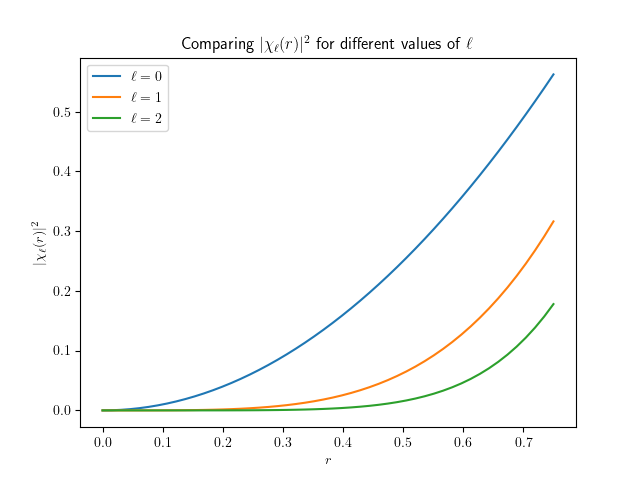
\includegraphics[scale=0.6]{chi_l_squared.png}
        \caption{\(\abs{\chi_\ell(r)}^2\) compared for \(\ell = 0, 1, 2\) and \(r < 1\).}
        \label{fig:chi for low r}
    \end{figure}
    Figure~\ref{fig:chi for low r} shows \(\abs{\chi_\ell(r)}^2\) plotted for \(\ell = 0, 1, 2\).
    We see that the larger the value of \(\ell\) the less likely the particle is to be near the origin.
    This can be see as analogous to the classical centrifugal potential which provides a force away from the origin.
    In quantum mechanics a centrifugal term in the potential instead decreases the probability of the particle being near the origin.
    
    There are two probabilities that we may be interested in.
    The \gls{pdf} for finding the particle at a specific point, \(\vv{r}\) is \(\abs{u(r, \vartheta, \varphi)}^2\) so the probability that the particle is in the volume \(\dd{V}\) is \(\abs{u(r, \vartheta, \varphi)}^2\dd{V}\).
    The probability that the particle is in a given volume, \(V\), is then
    \[\int_V \abs{u(r, \vartheta, \varphi)}^2.\]
    The \gls{pdf} for finding the particle at some specific radius, \(\vv{r}\) is \(\abs{\chi_\ell(r)}^2\) so the probability that the particle is at a point with radius \([r, r + \dd{r}]\) is
    \[\int\dd{\Omega}\abs{u(r, \vartheta, \varphi)}^2 = \int\dd{\Omega}\abs{Y_\ell^m(\vartheta, \varphi)}^2\abs{\chi_\ell(r)}^2\dd{r} = \abs{\chi_\ell(r)}^2\dd{r}.\]
    The probability that the particle is at some point with a radius in \([a, b]\) is then
    \[\int_a^b\dd{r}\abs{\chi_\ell(r)}^2.\]
    
    \section{Spin}
    We saw in section~\ref{sec:Bounds on m} that the angular momentum quantum number, \(\ell\), is always an integer despite the fact that the similarly defined \(j\) can take half integer values.
    This is because of the spatial dependence of the solutions.
    For the eigenfunctions of \(\operator{L}^2\) to be single valued we require that
    \[Y_\ell^m(\vartheta, \varphi) = Y_\ell^m(\vartheta, \varphi + 2\pi)\]
    and we saw that the \(\varphi\) dependence of \(Y_\ell^m\) was
    \[Y_\ell^m(\vartheta, \varphi) \propto e^{im\varphi}.\]
    In combination these two equations mean that \(m\) must be an integer.
    Since \(m\) takes on any value from \(-\ell\) to \(\ell\) this means that \(\ell\) must be an integer.
    
    \define{Spin} is an intrinsic property of a quantum system.
    It is like angular momentum in that the spin is associated with the operator
    \[\vecoperator{S} = (\operator{S}_1, \operator{S}_2, \operator{S}_3),\]
    with the commutation relation
    \[[\operator{S}_k, \operator{S}_l] = i\hbar\varepsilon_{klm}\operator{S}_m.\]
    This was the assumption that we made at the start of section~\ref{sec:algebraic solution to the eigenvalue problem} so we can use everything we derived in that section.
    In particular we can define 
    \[\operator{S}^2 = \operator{S}_x^2 + \operator{S}_y^2 + \operator{S}_z^2.\]
    \(\operator{S}^2\) and \(\operator{S}_z\) are a \gls{csco} and have a common eigenbasis:
    \[\left\{\ket{s, m}\st m = -s, 1 - s, \dotsc, s - 1, s~\text{and}~s = \frac{n}{2}~\text{where}~n\in\naturals\right\}.\]
    The action of \(\operator{S}^2\) and \(\operator{S}_z\) on these basis vectors is
    \[\operator{S}^2\ket{s, m} = s(s + 1)\hbar^2\ket{s, m}, \qquad\text{and}\qquad \operator{S}_z\ket{s, m} = m\hbar\ket{s, m}.\]
    For a fixed value of \(s\) we see that this is a \((2s + 1)\)-state system.
    
    From now on we focus only on spin 1/2 systems.
    That is systems where \(s = 1/2\).
    This includes electrons, protons, neutrons, neutrinos, and quarks.
    So most matter that we come across day to day.
    In this case we have a two dimensional vector space, \(\hilbert_{\text{spin}}\), with a basis
    \[\left\{\ket{\tfrac{1}{2}, \tfrac{1}{2}}, \ket{\tfrac{1}{2}, -\tfrac{1}{2}}\right\}.\]
    Since \(s = 1/2\) for both of these it is common to introduce a shorter notation where we refer to \(\ket{\tfrac{1}{2}, \tfrac{1}{2}}\) as spin up, denoted \(\ket{\tfrac{1}{2}}\) or \(\ket{\spinUp}\), and \(\ket{\tfrac{1}{2}, -\tfrac{1}{2}}\) as spin down, denoted \(\ket{-\tfrac{1}{2}}\) or \(\ket{\spinDown}\).
    These are still eigenfunctions of both \(\operator{S}^2\) and \(\operator{S}_z\):
    \[\operator{S}^2\ket{\spinUp} = \frac{3}{4}\hbar^2\ket{\spinUp}, \qquad, \operator{S}^2\ket{\spinDown} = \frac{3}{4}\hbar^2\ket{\spinDown},\]
    \[\operator{S}_z\ket{\spinUp} = \frac{\hbar}{2}, \qquad\text{and}\qquad \operator{S}_z\ket{\spinDown} = -\frac{\hbar}{2}\ket{\spinDown}.\]
    A generic spin state, \(\ket{\psi}\in\hilbert_\text{spin}\) is given by
    \[\ket{\psi} = \psi_1\ket{\spinUp} + \psi_2\ket{\spinDown}\]
    where as usual \(\psi_1 = \braket{\spinUp}{\psi}\), \(\psi_2 = \braket{\spinDown}{\psi}\), and \(\abs{\psi_1}^2 + \abs{\psi_2}^2 = 1\).
    Since spin has no spatial dependence we describe spin with vectors in \(\hilbert_\text{spin}\).
    If a system also has spatial dependence then we can describe this with vectors in some other vector space \(\hilbert_\text{space}\).
    The full description of a state is then given by a vector in
    \[\hilbert = \hilbert_\text{space}\tensorProd\hilbert_\text{spin}.\]
    \(\hilbert\) has as a basis
    \[\left\{ \ket{\vv{r}, m}\st \vv{r}\in\reals^3 ~\text{and}~ m = \pm\frac{1}{2} \right\}.\]
    The vectors in this basis are simply the tensor products of vectors of the individual bases of \(\hilbert_\text{space}\) and \(\hilbert_\text{spin}\):
    \[\ket{\vv{r}, m} = \ket{\vv{r}}\ket{m} = \ket{\vv{r}}\tensorProd\ket{m}.\]
    This basis is complete, meaning
    \[\int \dd[3]{r'} \sum_{m} \ketbra{\vv{r'}, m}{\vv{r'}, m} = \ident.\]
    A generic state, \(\ket{\psi}\in\hilbert\), is then given by
    \begin{align*}
        \ket{\psi} &= \int\dd[3]{r} \sum_m \ket{\vv{r'}, m}\braket{\vv{r'}, m}{\psi}\\
        &= \int\dd[3]{r'}\sum_m \psi_m(\vv{r'})\ket{\vv{r'}, m}\\
        &= \int\dd[3]{r'}\left[\psi_1(\vv{r'})\ket{\spinUp} + \psi_2(\vv{r'})\ket{\spinDown}\right]
    \end{align*}
    where \(\psi_m(\vv{r'}) = \braket{\vv{r'}, m}{\psi}\).
    Taking the inner product with a position eigenstate, \(\ket{\vv{r}}\), we have
    \begin{align*}
        \braket{\vv{r}}{\psi} &= \int \dd[3]{r'}\sum_m \braket{\vv{r}}{\vv{r'}}\ket{m}\psi_m(\vv{r'})\\
        &= \int \dd[3]{r'} \sum_m \delta(\vv{r} - \vv{r'})\ket{m}\psi_m(\vv{r'})\\
        &= \sum_m \int \dd[3]{r'} \delta(\vv{r} - \vv{r'})\ket{m}\psi_m(\vv{r'})\\
        &= \sum_m \psi_m(\vv{r})\\
        &= \psi_1(\vv{r})\ket{\spinUp} + \psi_2(\vv{r})\ket{\spinDown}.
    \end{align*}
    In the basis \(\{\ket{\spinUp}, \ket{\spinDown}\}\) for \(\hilbert_\text{spin}\) we can denote \(\braket{\vv{r}}{\psi}\) as a column vector:
    \[
        \braket{\vv{r}}{\psi} \representation 
        \begin{pmatrix}
            \psi_1(\vv{r})\\ \psi_2(\vv{r})
        \end{pmatrix}
        .
    \]
    The interpretation of these values is as follows:
    \begin{itemize}
        \item \(\abs{\psi_1(\vv{r})^2}\) -- the \gls{pdf} of finding the system at \(\vv{r}\) with spin up.
        \item \(\abs{\psi_2(\vv{r})^2}\) -- the \gls{pdf} of finding the system at \(\vv{r}\) with spin down.
        \item The probability of finding the system anywhere in space with spin up is
        \[P(\spinUp) = \int\dd[3]{r}\abs{\psi_1(\vv{r})}^2.\]
        \item The probability of finding the system anywhere in space with spin down is
        \[P(\spinDown) = \int\dd[3]{r}\abs{\psi_2(\vv{r})}^2.\]
        \item The probability of finding the system at \(\vv{r}\) with any spin is
        \[P(\vv{r}) = \abs{\psi_1(\vv{r})}^2 + \abs{\psi_2(\vv{r})}^2.\] 
    \end{itemize}
    
    \subsection{Matrix Elements}
    \(\hilbert_{\text{spin}}\) is a two-dimensional vector space.
    Therefore the spin operators can be represented by \(2\times 2\) matrices acting on column vectors.
    First we start with
    \[\operator{S}_z\ket{\spinUp} = \frac{\hbar}{2}\ket{\spinUp}, \qquad\text{and}\qquad \operator{S}_z\ket{\spinDown} = -\frac{\hbar}{2}\ket{\spinDown}.\]
    Hence
    \begin{align*}
        \bra{\spinUp}\operator{S}_z\ket{\spinUp} &= \frac{\hbar}{2},\\
        \bra{\spinUp}\operator{S}_z\ket{\spinDown} &= 0,\\
        \bra{\spinDown}\operator{S}_z\ket{\spinUp} &= 0,
        \shortintertext{and}
        \bra{\spinDown}\operator{S}_z\ket{\spinDown} &= -\frac{\hbar}{2}.
    \end{align*}
    This can be written compactly as
    \[\bra{m'}\operator{S}_z\ket{m} = \sign(m)\delta_{m'm}\frac{\hbar}{2}.\]
    Thus in this basis \(\operator{S}_z\) is represented by
    \[
        \operator{S}_z \representation \frac{\hbar}{2}
        \begin{pmatrix}
            1 & 0\\
            0 & -1
        \end{pmatrix}
        .
    \]
    Where we follow the convention that the first row (column) corresponds to the largest value of \(m'\) (\(m\)) so that the first row (column) is labelled by \(m' = 1/2\) (\(m = 1/2\)) and the second row (column) is labelled by \(m' = -1/2\) (\(m = -1/2\)).
    
    As before we define the operators
    \[\operator{S}_+ = \operator{S}_x + i\operator{S}_y, \qquad\text{and}\qquad \operator{S}_- = \operator{S}_x - i\operator{S}_y.\]
    These have the expected action that
    \[\operator{S}_+\ket{\spinUp} = 0, \qquad \operator{S}_+\ket{\spinDown} = \hbar c_+\ket{\spinUp} = \hbar \sqrt{\frac{1}{2}\left(\frac{1}{2} + 1\right) + \frac{1}{2}\left(-\frac{1}{2} + 1\right)}\ket{\spinUp} = \hbar\ket{\spinUp}\]
    \[\operator{S}_-\ket{\spinDown} = 0, \qquad\text{and}\qquad \operator{S}_-\ket{\spinUp} = \hbar c_-\ket{\spinDown} = \hbar\sqrt{\frac{1}{2}\left(\frac{1}{2} + 1\right) - \frac{1}{2}\left(\frac{1}{2} + 1\right)} = \hbar\ket{\spinDown}.\]
    Hence
    \begin{align*}
        \bra{\spinUp}\operator{S}_+\ket{\spinUp} = 0, \qquad & \bra{\spinUp}\operator{S}_-\ket{\spinUp} = 0,\\
        \bra{\spinUp}\operator{S}_+\ket{\spinDown} = \hbar, \qquad & \bra{\spinUp}\operator{S}_-\ket{\spinDown} = 0,\\
        \bra{\spinDown}\operator{S}_+\ket{\spinUp} = 0, \qquad & \bra{\spinDown}\operator{S}_-\ket{\spinUp} = \hbar,\\
        \bra{\spinDown}\operator{S}_+\ket{\spinDown} = 0, \qquad & \bra{\spinDown}\operator{S}_-\ket{\spinDown} = 0.
    \end{align*}
    Thus in this basis these operators are represented by
    \[
        \operator{S}_+ \representation\hbar
        \begin{pmatrix}
            0 & 1\\
            0 & 0
        \end{pmatrix}
        \qquad\text{and}\qquad
        \operator{S}_- \representation\hbar
        \begin{pmatrix}
            0 & 0\\
            1 & 0
        \end{pmatrix}
        .
    \]
    Now we can write
    \[\operator{S}_x = \frac{1}{2}\left(\operator{S}_+ + \operator{S_-}\right), \qquad\text{and}\qquad \operator{S}_y = \frac{1}{2i}\left(\operator{S}_+ - \operator{S}_-\right).\]
    Thus the representations of \(\operator{S}_x\) and \(\operator{S}_y\) in this basis are
    \[
        \operator{S}_x \representation \frac{\hbar}{2}
        \begin{pmatrix}
            0 & 1\\
            1 & 0
        \end{pmatrix}
        \qquad\text{and}\qquad
        \operator{S}_y \representation \frac{\hbar}{2}
        \begin{pmatrix}
            0 & -i\\
            i & 0
        \end{pmatrix}
        .
    \]
    The three matrices representing \(\operator{S}_k\) in this basis are called the \define{Pauli spin matrices}:
    \[
        \sigma_x =
        \begin{pmatrix}
            0 & 1\\
            1 & 0
        \end{pmatrix}
        ,\qquad \sigma_y =
        \begin{pmatrix}
            0 & -i\\
            i & 0
        \end{pmatrix}
        ,\qquad\text{and}\qquad \sigma_z = 
        \begin{pmatrix}
            1 & 0\\
            0 & 1
        \end{pmatrix}
        .
    \]
    Which allows us to compactly write
    \[\operator{S}_k \representation \frac{\hbar}{2}\sigma_k, \qquad\text{and}\qquad \vecoperator{S} = \frac{\hbar}{2}\vv{\sigma}\]
    where \(\vv{\sigma} = (\sigma_x, \sigma_y, \sigma_z)\).
    The Pauli matrices are Hermitian, as they are associated with observables, and also unitary, meaning \(\sigma_k\sigma_k\hermit = \sigma_k^2 = \ident\), they also all have zero trace, \(\tr(\sigma_k) = 0\).
    We can then use \(\sigma\) as another label for the basis vectors, for example if we define
    \[\ket{\psi} = \sum_{\sigma} \psi_\sigma\ket{\sigma}\]
    then we can characterise the action of \(\operator{S}_k\) as
    \[\ket{\varphi} = \operator{S}_k = \sum_\sigma \varphi_\sigma\ket{\sigma} = \sum_\sigma\sum_{\sigma'}(S_k)_{\sigma\sigma'}\psi_{\sigma'}\ket{\sigma}\]
    where we have used
    \[\varphi_\sigma = \sum_{\sigma'}(S_k)_{\sigma\sigma'}\psi_{\sigma'}.\]
    
    We can now use the definition of \(\operator{S}^2\) to find a representation for \(\operator{S}^2\) in this basis:
    \begin{align*}
        \operator{S}^2 &= \sum_k \operator{S}_k^2\\
        &\representation \sum_k \left(\frac{\hbar}{2}\sigma_k\right)^2\\
        &= \sum_k \frac{\hbar^2}{4}\sigma_k^2\\
        &= \sum_k \frac{\hbar^2}{4}\ident\\
        &= \frac{3}{4}\hbar^2\ident\\
        &= \frac{3}{4}\hbar^2
        \begin{pmatrix}
            1 & 0\\
            0 & 1
        \end{pmatrix}
    \end{align*}
    
    \subsection{Eigenvectors of \texorpdfstring{\(\operator{S}_z\)}{Sz} and \texorpdfstring{\(\operator{S}^2\)}{S2}}
    The eigenvectors of \(\sigma_z\) are easy to find:
    \[
        \begin{pmatrix}
            1 & 0\\
            0 & -1
        \end{pmatrix}
        \begin{pmatrix}
            1\\ 0
        \end{pmatrix}
        =
        \begin{pmatrix}
            1\\ 0
        \end{pmatrix}
        ,\qquad\text{and}\qquad
        \begin{pmatrix}
            1 & 0\\
            0 & -1
        \end{pmatrix}
        \begin{pmatrix}
            0\\ 1
        \end{pmatrix}
        = -
        \begin{pmatrix}
            0\\ 1
        \end{pmatrix}
        .
    \]
    So the eigenvalues of this representation of \(\operator{S}_z\) are given by
    \[
        \frac{\hbar}{2}
        \begin{pmatrix}
            1 & 0\\
            0 & -1
        \end{pmatrix}
        \begin{pmatrix}
            1\\ 0
        \end{pmatrix}
        = \frac{\hbar}{2}
        \begin{pmatrix}
            1\\ 0
        \end{pmatrix}
        ,\qquad\text{and}\qquad
        \frac{\hbar}{2}
        \begin{pmatrix}
            1 & 0\\
            0 & -1
        \end{pmatrix}
        \begin{pmatrix}
            0\\ 1
        \end{pmatrix}
        = -\frac{\hbar}{2}
        \begin{pmatrix}
            0\\ 1
        \end{pmatrix}
        .
    \]
    We see that these have the eigenvalues \(\pm\hbar/2\), which is what we would expect for a spin 1/2 system.
    These eigenvectors are also simultaneously eigenvectors of \(\operator{S}^2\) in this representation, this is trivial since \(\operator{S}^2\) is proportional to the identity in this representation:
    \[
        \frac{3}{4}\hbar^2
        \begin{pmatrix}
            1 & 0\\
            0 & 1
        \end{pmatrix}
        \begin{pmatrix}
            1\\ 0
        \end{pmatrix}
        = \frac{3}{4}\hbar^2
        \begin{pmatrix}
            1\\ 0
        \end{pmatrix}
        ,\qquad\text{and}\qquad
        \frac{3}{4}\hbar^2
        \begin{pmatrix}
            1 & 0\\
            0 & 1
        \end{pmatrix}
        \begin{pmatrix}
            0\\ 1
        \end{pmatrix}
        = \frac{3}{4}\hbar^2
        \begin{pmatrix}
            0\\ 1
        \end{pmatrix}
        .
    \]
    Thus we can identify
    \[
        \ket{s=\tfrac{1}{2}, m=\tfrac{1}{2}} = \ket{\spinUp} \representation 
        \begin{pmatrix}
            0\\ 1
        \end{pmatrix}
        ,\qquad\text{and}\qquad
        \ket{s = \tfrac{1}{2}, m=-\tfrac{1}{2}} = \ket{\spinDown} \representation
        \begin{pmatrix}
            1\\ 0
        \end{pmatrix}
        .
    \]
    A generic vector, \(\ket{\psi}\in\hilbert_{\text{spin}}\), can then be represented by
    \[
        \ket{\psi} = \psi_1\ket{\spinUp} + \psi_2\ket{\spinDown} \representation
        \begin{pmatrix}
            \psi_1\\
            \psi_2
        \end{pmatrix}
        =
        \psi_1
        \begin{pmatrix}
            1\\ 0
        \end{pmatrix}
        + \psi_2
        \begin{pmatrix}
            0\\ 1
        \end{pmatrix}
        .
    \]
    Note that in general \(\psi_k\in\complex\) so the space spanned by these eigenvectors is not \(\reals^2\) but \(\complex^2\).
    
    \subsection{Scalar Products}
    Now that we have representations of generic vectors in this basis we ask what is the representation of a covector, \(\bra{\psi}\in\hilbert_{\text{spin}}^*\)?
    The answer, as always, is that if \(\ket{\psi}\) is represented by an \(n\)-dimensional column vector then \(\bra{\psi}\) is represented by an \(n\)-dimensional row vector with the components given by
    \[
        \ket{\psi} \representation 
        \begin{pmatrix}
            \psi_1\\ \psi_2
        \end{pmatrix}
        \implies
        \bra{\psi} \representation
        \begin{pmatrix}
            \psi_1^* & \psi_2^*
        \end{pmatrix}
        .
    \]
    That is \(\bra{\psi} = (\ket{\psi})\hermit\).
    The scalar product of two states, \(\ket{\psi}\) and \(\ket{\varphi}\), is then
    \[
        \braket{\varphi}{\psi} =
        \begin{pmatrix}
            \varphi_1^* & \varphi_2^*
        \end{pmatrix}
        \begin{pmatrix}
            \psi_1\\ \psi_2
        \end{pmatrix}
        = \varphi_1^*\psi_1 + \varphi_2^*\psi_2.
    \]
    For example if \(\ket{\psi}\) is a properly normalised state then
    \[
        \braket{\varphi}{\psi} =
        \begin{pmatrix}
            \psi_1^* & \psi_2^*
        \end{pmatrix}
        \begin{pmatrix}
            \psi_1\\ \psi_2
        \end{pmatrix}
        = \abs{\psi_1}^2 + \abs{\varphi_2}^2  = 1.
    \]
    
    \subsection{Spin Along the \texorpdfstring{\(x\)}{x} Direction}
    We can find the possible values of \(m_x\) by finding the eigenvalues of \(\hbar\sigma_x/2\) in the \(\operator{S}_z\) eigenbasis.
    We do this in the normal way:
    \begin{align*}
        0 &= \det\left(\frac{\hbar}{2}\sigma_x - \lambda\ident\right)\\
        &= 
        \begin{vmatrix}
            -\lambda & \hbar/2\\
            \hbar/2 & -\lambda
        \end{vmatrix}
        \\
        &= \lambda^2 - \frac{\hbar^2}{4}
    \end{align*}
    So \(S_x = \lambda = \pm \hbar/2\).
    This is the same as the possible values of \(S_z\), this is what we would expect from the symmetry of the situation, there is nothing important about the \(z\) or \(x\) directions that would mean they have different possible values of \(S_k\).
    We can write a state with \(m_x = 1/2\) as a combination of the basis vectors:
    \[\ket{m_x = 1/2} = \alpha\ket{\spinUp} + \beta\ket{\spinDown}.\]
    In this representation this becomes
    \[
        \operator{S}_x\ket{m_x = 1/2} = \frac{\hbar}{2}\ket{m_x = 1/2} \representation \frac{\hbar}{2}\sigma_x
        \begin{pmatrix}
            \alpha\\ \beta
        \end{pmatrix}
        =
        \frac{\hbar}{2}
        \begin{pmatrix}
            0 & 1\\
            1 & 0
        \end{pmatrix}
        \begin{pmatrix}
            \alpha\\ \beta
        \end{pmatrix}
        = \frac{\hbar}{2}
        \begin{pmatrix}
            \beta\\ \alpha
        \end{pmatrix}
        = \frac{\hbar}{2}
        \begin{pmatrix}
            \alpha\\ \beta
        \end{pmatrix}
        .
    \]
    Hence \(\alpha = \beta\) so a properly normalised state with \(m_x = \hbar/2\) is
    \[\ket{m_x = 1/2} = \frac{\sqrt{2}}{2}\left[\ket{\spinUp} + \ket{\spinDown}\right].\]
    We can show in a similar way that if \(S_x = -1/2\) then
    \[\ket{m_x = -1/2} = \frac{\sqrt{2}}{2}\left[\ket{\spinUp} - \ket{\spinDown}\right].\]
    
    It can be shown that if we measure the spin along any vector in the \((x, z)\)-plane at an angle \(\vartheta\) to the \(z\) axis,
    \[\vh{n} = \sin(\vartheta)\ve{x} + \cos(\vartheta)\ve{z},\]
    then the relevant eigenstates in the the representation that we are using are the eigenvalues of
    \[
        \vv{\sigma}\cdot\vh{n} = \sigma_x\sin(\vartheta) + \sigma_z\cos(\vartheta) = 
        \begin{pmatrix}
            \cos\vartheta & \sin\vartheta\\
            \sin\vartheta & -\cos\vartheta
        \end{pmatrix}
        .
    \]
    
    \section{Addition of Angular Momenta}\label{sec:addition of angular momenta}
    Suppose we have two systems with independent angular momenta \(\vecoperator{J}^{(1)}\) and \(\vecoperator{J}^{(2)}\).
    This could be two particles with angular momentum, two particles with spin or one particle with angular momentum and spin.
    These operators satisfy the usual commutation relations,
    \[\left[\operator{J}^{(n)}_k, \operator{J}^{(n)}_l\right] = i\hbar\varepsilon_{klm}\operator{J}^{(n)}_m, \qquad\text{and}\qquad \left[\angmomsquared{n}, \operator{J}^{(n)}_k\right] = 0.\]
    Since the two angular momenta are independent the operators associated with different angular momenta commute:
    \[\left[\operator{J}^{(1)}_k, \operator{J}^{(2)}_l\right] = \left[\angmomsquared{1}, \angmomsquared{2}\right] = \left[\angmomsquared{1}, \operator{J}^{(2)}_k\right] = 0 \qquad\text{etc.}\]
    We can extend this easily to any number of independent angular momenta but we won't here.
    
    \subsection{Vector Spaces}
    Since \(\vecoperator{J}^{(1)}\) and \(\vecoperator{J}^{(2)}\) commute they form a \gls{csco} which means we can find a common eigenbasis.
    Since both angular momenta are independent we can describe both with separate Hilbert spaces.
    Angular momentum 1 is described by vectors in a vector space \(\hilbert^{(1)}\).
    For a particular value, \(j^{(1)}\), of the angular momentum quantum number this is a \(2j_1 + 1\) dimensional vector space.
    This space has as a basis \(\{\ket{j_1, m_1}\}\)
    Similarly angular momentum 2 is described by vectors in the \(2j_2 + 1\) dimensional vector space, \(\hilbert^{(2)}\), with basis \(\ket{j_2, m_2}\).
    The entire system is then described by vectors in
    \[\hilbert = \hilbert^{(1)}\tensorProd\hilbert^{(2)}.\]
    The dimensionality of this vector space is
    \[\dim(\hilbert) = \dim(\hilbert^{(1)})\dim(\hilbert^{(2)}) = (2j_1 + 1)(2j_2 + 1).\]
    This space then has as a basis
    \[\{\ket{j_1, m_1, j_2, m_2}\} = \{\ket{j_1, m_1}\tensorProd\ket{j_2, m_2}\}.\]
    As usual we extend the definition of the operators so that they act on only their respective parts of these vectors.
    Strictly we should define new operators like \({\operator{J}^{(1)}_z}{'} = \operator{J}^{(1)}_z\tensorProd\ident\) which then acts on \(\ket{j_1, m_1, j_2, m_2} = \ket{j_1, m_1}\tensorProd\ket{j_2, m_2}\) as
    \begin{align*}
        {\operator{J}^{(1)}_z}{'}\ket{j_1, m_1, j_2, m_2} &= (\operator{J}^{(1)}_z\tensorProd\ident)(\ket{j_1, m_1}\tensorProd\ket{j_2, m_2})\\
        &= \operator{J}^{(1)}_z\ket{j_1, m_1}\tensorProd\ident\ket{j_2, m_2}\\
        &= \hbar m_1\ket{j_1, m_1}\tensorProd\ket{j_2, m_2}\\
        &= \hbar m_1\ket{j_1, m_1, j_2, m_2}
    \end{align*}
    but in practice we use the same symbol for both operators, \(\operator{J}^{(1)}_z\colon\hilbert^{(1)}\to\complex\) and \(\operator{J}^{(1)}_z{'}\colon\hilbert\to\complex\).
    The action of the operators on this basis is
    \begin{align*}
        \angmomsquared{1}\ket{j_1, m_1, j_2, m_2} &= \hbar^2j_1(j_1 + 1)\ket{j_1, m_1, j_2, m_2},\\
        \operator{J}^{(1)}_z\ket{j_1, m_1, j_2, m_2} &= \hbar m_1\ket{j_1, m_1, j_2, m_2},\\
        \angmomsquared{2}\ket{j_1, m_1, j_2, m_2} &= \hbar^2j_2(j_2 + 1)\ket{j_1, m_1, j_2, m_2},\\
        \operator{J}^{(2)}_z\ket{j_1, m_1, j_2, m_2} &= \hbar m_2\ket{j_1, m_1, j_2, m_2}.
    \end{align*}
    A generic state, \(\ket{\psi}\in\hilbert\), can be given as
    \[\ket{\psi} = \sum_{j_1, m_2, j_2, m_2} c_{j_1m_1j_2m_2}\ket{j_1, m_1, j_2, m_2}\]
    where
    \[c_{j_1m_1j_2m_2} = \braket{j_1, m_1, j_2, m_2}{\psi}.\]
    
    \subsection{Total Angular Momentum}\label{sec:total angular momentum}
    We can now define the total angular momentum:
    \[\vecoperator{J} = \vecoperator{J}^{(1)} + \vecoperator{J}^{(2)}.\]
    This satisfies the normal angular momentum commutation relations:
    \[[\operator{J}_k, \operator{J}_l] = i\hbar\varepsilon_{klm}\operator{J}_m, \qquad\text{and}\qquad [\operator{J}^2, \operator{J}_k] = 0.\]
    This means that \(\operator{J}^2\) and \(\operator{J}_z\) form a \gls{csco} so we can find a simultaneous eigenbasis for \(\hilbert\) made of vectors of the form \(\{\ket{j, m}\}\).
    What values can \(j\) and \(m\) take?
    The answer lies in the angular momentum addition theorem, which we won't prove here:
    \begin{theorem}[Angular momentum addition theorem]
        Given two independent angular momenta with corresponding quantum numbers, \(j_1\) and \(j_2\), the allowed value of the angular momentum quantum number for the total angular momentum are
        \[j = j_1 + j_2, j_1 + j_2 - 1, \dotsc, \abs{j_1 - j_2}.\]
        For each of these values we also have
        \[m = -j, -j + 1, \dotsc, j - 1, j.\]
    \end{theorem}
    Before we said that \(\dim(\hilbert) = (2j_1 + 1)(2j_2 + 1)\).
    We can check that this is consistent with the angular momentum addition theorem.
    Without loss of generality assume that \(j_1 \ge j_2\).
    Then
    \begin{align*}
        \dim(\hilbert) &= \sum_{\mathclap{j=j_1 - j_2}}^{\mathclap{j_1 + j_2}} (2j + 1)\\
        &= \sum_{j=0}^{\mathclap{j_1 + j_2}} (2j + 1) - \sum_{j = 0}^{\mathclap{j_1 - j_2 - 1}} (2j + 1)\\
        &= 2\sum_{j=0}^{\mathclap{j_1 + j_2}} j + (j_1 + j_2) - 2\sum_{j = 0}^{\mathclap{j_1 - j_2 - 1}} j - (j_1 - j_2 - 1 )\\
        &= (j_1 + j_2)(j_1 + j_2 + 1) + (j_1 + j_2) - (j_1 - j_2 - 1)(j_1 - j_2) - (j_1 - j_2 - 1)\\
        &= j_1^2 + j_2^2 + 2j_1j_2 + j_1 + j_2 + j_1 + j_2 - j_1^2 - j_2^2 + 2j_1j_2 + j_1 - j_2 - j_1 + j_2 + 1\\
        &= 4j_1j_2 + 2j_1 + 2j_2 + 1\\
        &= (2j_1 + 1)(2j_2 + 1).\\
    \end{align*}
    Where we have used
    \[\sum_{r = 0}^n = \frac{1}{2}n(n + 1),\]
    which is proven in appendix~\ref{sec:proof sum 0 to n of r is 0.5 n(n+1)}.
    Both bases, \(\{\ket{j_1, m_1, j_2, m_2}\}\) and \(\{\ket{j, m}\}\), are orthonormal so there exists a unitary transformation between the two bases.
    For fixed \(j_1\) and \(j_2\) we denote \(\ket{j, m}\) as \(\ket{j, m; j_1, j_2}\) to denote the specific values that \(j_1\) and \(j_2\) are held at.
    Using the completeness of the \(\{\ket{j_1, m_1, j_2, m_2}\}\) basis,
    \[\sum_{m_1, m_2} \braket{j_1, m_1, j_2, m_2}{j_1, m_1, j_2, m_2} = \ident\]
    we have
    \[\ket{j, m; j_1, j_2} = \sum_{m_1, m_2} \ket{j_1, m_1, j_2, m_2}\braket{j_1, m_1, j_2, m_2}{j, m; j_1, j_2}.\]
    The quantities \(\braket{j_1, m_1, j_2, m_2}{j, m; j_1, j_2}\) are called the Clebsch--Gordan coefficients and they are tabulated in many sources.
    
    The basis \(\{\ket{j_1, m_1, j_2, m_2}\}\) is called the \define{uncoupled basis} as vectors in this basis can be written as two parts, one related to angular momentum 1 and the other related to angular momentum 2, for example a basis vector can be written as \(\ket{j_1, m_1}\tensorProd\ket{j_2, m_2}\) and a generic vector as
    \[\ket{\psi} = \sum_{\mathclap{j_1, m_1, j_2, m_2}}(\braket{j_1, m_1}{\psi}\ket{j_1, m_1} \tensorProd\braket{j_2, m_2}{\psi}\ket{j_2, m_2}).\]
    The basis \(\{\ket{j, m}\}\) is called the \define{coupled basis} as this is not possible.
    
    \begin{example}
        Consider a system composed of two spin 1/2 particles.
        \(\hilbert^{(1)}\) is a two dimensional vector space with a basis
        \[\{s_1, m_1\} = \{\ket{\tfrac{1}{2}, \tfrac{1}{2}}, \ket{\tfrac{1}{2}, -\tfrac{1}{2}}\}.\]
        \(\hilbert^{(2)}\) is also a two dimensional vector space with basis
        \[\{s_2, m_2\} = \{\ket{\tfrac{1}{2}, \tfrac{1}{2}}, \ket{\tfrac{1}{2}, -\tfrac{1}{2}}\}.\]
        The spin of the whole system is then characterised by vectors in \(\hilbert = \hilbert^{(1)}\tensorProd\hilbert^{(2)}\) which has the basis
        \[\{\ket{s_1, m_1, s_2, m_2}\} = \{\ket{\tfrac{1}{2},\tfrac{1}{2},\tfrac{1}{2},\tfrac{1}{2}}, \ket{\tfrac{1}{2},\tfrac{1}{2},\tfrac{1}{2},-\tfrac{1}{2}}, \ket{\tfrac{1}{2},-\tfrac{1}{2},\tfrac{1}{2},\tfrac{1}{2}}, \ket{\tfrac{1}{2},-\tfrac{1}{2},\tfrac{1}{2},-\tfrac{1}{2}}\}.\]
        Since \(s_i = 1/2\) for all states in this system we compactly write this basis as
        \[\{\ket{\spinUp\spinUp}, \ket{\spinUp\spinDown}, \ket{\spinDown\spinUp}, \ket{\spinDown, \spinDown}\}.\]
        Where the first arrow denotes particle 1's spin and the second arrow denotes particle 2's spin.
        The values that \(s\) can take, as given by the angular momentum addition theorem, is \(s = s_1 + s_2, \abs{s_1 - s_2} = 1, 0\).
        So the entire system has spin 1 or spin 0.
        To find the uncoupled basis consider the action of \(\operator{S}_z\) on the coupled basis
        \[\operator{S}_z\ket{\spinUp\spinUp} = (\operator{S}^{(1)}_z + \operator{S}^{(2)}_z)\ket{\spinUp\spinUp} = \frac{\hbar}{2}\ket{\spinUp\spinUp} + \frac{\hbar}{2}\ket{\spinUp\spinUp} = \hbar\ket{\spinUp\spinUp}.\]
        Hence \(m = 1\).
        Since \(m > 0\) we know that \(s \ne 0\) so \(s = 1\).
        Similarly
        \[\operator{S}_z\ket{\spinDown\spinDown} = (\operator{S}^{(1)}_z + \operator{S}^{(2)}_z)\ket{\spinDown\spinDown} = -\frac{\hbar}{2}\ket{\spinDown\spinDown} + -\frac{\hbar}{2}\ket{\spinDown\spinDown} = -\hbar\ket{\spinDown\spinDown}.\]
        Hence \(m = 1\) and \(s = 1\) for this state.
        So far we have
        \[\ket{1,1} = \ket{\spinUp\spinUp}, \qquad\text{and}\qquad \ket{1,-1} = \ket{\spinDown\spinDown}.\]
        We don't yet know what \(\ket{1, 0}\) or \(\ket{0, 0}\) are.
        The difficulty in finding these states is that they aren't uniquely identified purely by the value of \(m\).
        However we do know how to construct them from other states using raising and lowering operators.
        The lowering operator for the total angular momentum is simply
        \[\operator{S}_- = \operator{S}^{(1)}_- + \operator{S}^{(2)}_-\]
        so by identifying that we expect
        \[\operator{S}_-\ket{1, 1} \propto \ket{1, 0}\]
        we know that
        \[\ket{1, 0} \propto \operator{S}_-\ket{\spinUp\spinUp} = (\operator{S}^{(1)}_- + \operator{S}^{(2)}_-)\ket{\spinUp\spinUp} = \operator{S}^{(1)}_-\ket{\spinUp\spinUp} + \operator{S}^{(2)}_-\ket{\spinUp\spinUp} \propto \ket{\spinDown\spinUp} + \ket{\spinUp\spinDown}.\]
        Using the fact that the uncoupled basis vectors are orthonormal we have
        \[\ket{1, 0} = \frac{\sqrt{2}}{2}(\ket{\spinUp\spinDown} + \ket{\spinUp\spinDown}).\]
        Finally \(\ket{0, 0}\) must be a linear combination of \(\ket{\spinUp\spinDown}\) and \(\ket{\spinDown\spinUp}\) and it must be orthogonal to \(\ket{1, 0}\).
        We are then free to chose that
        \[\ket{0, 0} = \frac{\sqrt{2}}{2}(\ket{\spinUp\spinDown} - \ket{\spinDown\spinUp}).\]
        This agrees with the Clebsch--Gordan coefficients which are tabulated in table~\ref{tab:clebsch-gordan coefficients j = 1}.
        \begin{table}[ht]
            \centering
            \begin{subtable}{0.25\textwidth}
                \centering
                \begin{tabular}{|l|l|}\hline
                    \backslashbox{\(m_1, m_2\)}{\(j\)} & 1\\ \hline
                    \(1/2, 1/2\) & 1\\ \hline
                \end{tabular}
                \subcaption{\(m = 1\)}
            \end{subtable}
            \begin{subtable}{0.25\textwidth}
                \centering
                \begin{tabular}{|l|l|}\hline
                    \backslashbox{\(m_1, m_2\)}{\(j\)} & 1\\ \hline
                    \(-1/2, -1/2\) & 1\\ \hline
                \end{tabular}
                \subcaption{\(m = -1\)}
            \end{subtable}
            \begin{subtable}{0.4\textwidth}
                \centering
                \begin{tabular}{|l|l|l|}\hline
                    \backslashbox{\(m_1, m_2\)}{\(j\)} & 1 & 0\\ \hline
                    \(1/2, -1/2\) & \(\sqrt{2}/2\) & \(\sqrt{2}/2\)\\ \hline
                    \(-1/2, 1/2\) & \(\sqrt{2}/2\) & -\(\sqrt{2}/2\)\\ \hline
                \end{tabular}
                \subcaption{\(m = 0\)}
            \end{subtable}
            
            
            \caption{Clebsch--Gordan coefficients for two spin 1/2 particles.}
            \label{tab:clebsch-gordan coefficients j = 1}
        \end{table}
    \end{example}

    \section{Identical Particles}
    In classical mechanics if we have two particles that have all the same properties, like mass, charge, angular momentum, etc. then we can still tell them apart from the fact that one of them is `here' and the other is `there'.
    Even at some later time we can still tell them apart as we can track their trajectories back to a time when we could tell them apart.
    In \gls{qm} this is not possible.
    If two particles have the same properties, meaning identical quantum numbers, \(n\), \(\ell\), \(s\), \(m\), etc. then we label one `particle 1' and the other `particle 2' we lose this information as soon as we ascribe it as the system evolves and since there is no concept of trajectory we can't tell which particle was which at some earlier time.
    
    To think about this mathematically we start with the states, \(\ket{\xi_1}, \ket{\xi_2}\in\hilbert\), which describe each particle.
    The two particle system is then described by \(\ket{\xi_1, \xi_2} = \ket{\xi_1}\tensorProd\ket{\xi_2} \in\hilbert \tensorProd\hilbert\).
    
    Here particle 1 and 2 are labels that we assign that distinguish the particles for the sake of the maths.
    There is no way to look at a particle and tell if it is particle 1 or 2.
    We define an operator, \(\operator{\parity}_{12}\) which swaps particle 1 and 2.
    That is
    \[\operator{\parity}_{12}\ket{\xi_1, \xi_2} = \ket{\xi_2, \xi_1}.\]
    Since quantum states are defined up to a phase factor and swapping the two particles doesn't change the state of the system we must have that
    \[\ket{\xi_1, \xi_2} = e^{i\alpha}\ket{\xi_2, \xi_1}\]
    for some \(\alpha\in\reals\).
    By swapping the two states again we get back to the original state and we pick up another phase factor:
    \[\ket{\xi_1, \xi_2} = e^{2i\alpha}\ket{\xi_1, \xi_2}.\]
    This can only be true if \(e^{2i\alpha} = 1\) which means that \(e^{i\alpha} = \pm 1\), thus \(\alpha = n\pi\) for \(n\in\integers\).
    This means that this state is either symmetric or antisymmetric under swapping the particles.
    It turns out that there is a theorem that allows us to be even more precise than this, which we will not prove here.
    It is called the spin statistics theorem:
    \begin{theorem}[Spin statistics theorem]
        Particles with integer spin, \(s = 0, 1, 2, \dotsc\), are symmetric under swapping identical particles:
        \[\ket{\xi_1, \xi_2} = \ket{\xi_2, \xi_1}.\]
        Such particles are called \define{bosons} and are described by Bose--Einstein statistics.
        
        Particles with half integer spin, \(s = 1/2, 3/2, 5/2, \dotsc\), are antisymmetric under swapping identical particles:
        \[\ket{\xi_1, \xi_2} = - \ket{\xi_2, \xi_1}.\]
        Such particles are called \define{fermions} and are described by Fermi--Dirac statistics.
    \end{theorem}

    \subsection{Helium Atom}
    A helium atom, \ce{He}, has two electrons.
    These electrons are identical particles.
    There is also a proton.
    The interaction of one electron and the proton has a Hamiltonian given by
    \[\operator{H}_i = \frac{\vecoperator{P}\cdot\vecoperator{P}}{2\mu} - \frac{2e^2}{r_i}\]
    where \(i = 1, 2\) denotes the particle number, \(\mu\) is the mass of the electron, \(e\) is the magnitude of the charge of the electron and proton, and \(r_i\) denotes the distance of electron \(i\) from the proton.
    The entire system can then be described as the Hamiltonian for each electron plus a term characterising the interaction of the two electrons:
    \[\operator{H} = \operator{H}_1 + \operator{H}_2 + \frac{e^2}{\abs{\vv{r_1} - \vv{r_2}}}.\]
    Notice that \(\operator{H}\) is symmetric under \(\operator{\parity}_{12}\).
    That is \(\operator{H}(1, 2) = \operator{H}(2, 1)\) where \(\operator{H}(1, 2)\) is \(\operator{H}\) as defined above and \(\operator{H}(2, 1) = \operator{\parity}_{12}\operator{H}(1, 2)\).
    The \gls{tise} for this system is
    \[\operator{H}(1, 2)\ket{\xi_1, \xi_2} = E\ket{\xi_1, \xi_2},\]
    where we now require that \(\ket{\xi_1, \xi_2}\) is an energy eigenstate.
    We now rename 1 to 2 and 2 to 1, this changes nothing other than labels:
    \[\operator{H}(2, 1)\ket{\xi_2, \xi_1} = E\ket{\xi_2, \xi_1}.\]
    Finally using the fact that \(\operator{H}(1, 2) = \operator{H}(2, 1)\) we have that
    \[\operator{H}(1, 2)\ket{\xi_2, \xi_2} = E\ket{\xi_2, \xi_2}.\]
    Thus any given eigenstate, \(\ket{\xi_1, \xi_2}\), of \(\operator{H}(1, 2)\), gives us another eigenstate, \(\ket{\xi_2, \xi_1}\).
    We can define a symmetric and antisymmetric state, \(\ket{+}\) and \(\ket{-}\) respectively, in the usual way:
    \[\ket{\psi\pm} = \frac{\sqrt{2}}{2}(\ket{\xi_1, \xi_2} \pm \ket{\xi_2, \xi_1}).\]
    The action of \(\operator{\parity}_{12}\) on these is
    \[\operator{\parity}_{12}\ket{\pm} = \pm\ket{\pm}.\]
    So \(\ket{\pm}\) are eigenstates of \(\operator{\parity}_{12}\), with eigenvalues \(\pm 1\) and \(\operator{H}\), with eigenvalues \(E\).
    Hence \([\operator{H}, \operator{\parity}_{12}] = 0\).
    This means that the symmetry properties of the system are preserved in time since this means that \(\operator{\parity}_{12}\) commutes with the time evolution operator.
    
    \subsection{Two Electron State}
    Consider now a system made of two electrons.
    There are sets of degrees of freedom to consider.
    The spatial degrees of freedom, described by vectors in \(\hilbert_{\text{space}}\), and the spin degrees of freedom, described by vectors in \(\hilbert_{\text{spin}}\).
    Both electrons have \(s_i = 1/2\) so by the angular momenta addition theorem the total spin of the system is \(s = 0, 1\).
    In the case where \(s = 0\) we must also have \(m = 0\) so \(\ket{0, 0}\) is the only state with \(s = 0\), we call this a singlet state.
    In the case where \(s = 1\) we have \(m = -1, 0, 1\) so there are three states, \(\ket{1, -1}\), \(\ket{1, 0}\), and \(\ket{1, 1}\), with \(s = 1\), we call this a triplet state.
    We have previously shown that in the uncoupled basis these states are
    \[\ket{0, 0} = \frac{\sqrt{2}}{2}(\ket{\spinUp\spinDown} - \ket{\spinDown\spinUp}), \qquad \ket{1, 1} = \ket{\spinUp\spinUp}, \qquad \ket{1, -1} = \ket{\spinDown\spinDown}, \qquad\text{and}\qquad \ket{1, 0} = \frac{\sqrt{2}}{2}(\ket{\spinUp\spinDown} + \ket{\spinDown\spinUp}).\]
    From this we can see that \(\ket{0, 0}\) is antisymmetric under swapping of the two particles and all the other states are symmetric.
    Let \(\ket{\psi_{12}}\hilbert_{\text{space}}\) be a generic state describing the spatial degrees of freedom.
    The a generic state, \(\ket{\Psi} \in \hilbert = \hilbert_{\text{space}}\tensorProd\hilbert_{\text{spin}}\) with \(s = 1\) is given by
    \[\ket{\Psi} = \ket{\psi_{12}}\tensorProd\ket{s=1, m}.\]
    Using the fact that \(s = 1\) implies that \(\ket{s=1, m}\) is symmetric under \(\operator{\parity}_{12}\) the action of swapping the two particles is given by
    \begin{align*}
        \operator{\parity}_{12}\ket{\Psi} &= (\operator{\parity}_{12}\ket{\psi_{12}}) \tensorProd (\operator{\parity}_{12}\ket{s=1, m})\\
        &= (\operator{\parity}_{12}\ket{\psi_{12}}) \tensorProd \ket{s=1, m}\\
        &= -\ket{\Psi}.
    \end{align*}
    Here we have used that electrons are spin 1/2 particles so by the spin statistics theorem the overall state describing them is antisymmetric.
    The only way to have this be true is to have \(\ket{\psi_{12}}\) be antisymmetric under \(\operator{\parity_{12}}\).
    Similarly a generic state with \(s=0\) is described by
    \[\ket{\Psi} = \ket{\psi_{12}}\tensorProd\ket{s=0, m=0}.\]
    Again this is antisymmetric under \(\operator{\parity_{12}}\) but this time \(\ket{s=0, m=0}\) is antisymmetric under \(\operator{\parity_{12}}\) so \(\ket{\psi_{12}}\) must be symmetric under \(\operator{\parity_{12}}\).
    These two results are tabulated in table~\ref{tab:symmetry under swapping of particles}.
    \begin{table}[ht]
        \centering
        \begin{tabular}{cccc}\hline
            \(s\) & \(\ket{s, m}\) & \(\ket{\psi_{12}}\) & \(\ket{\Psi}\)\\\hline
            0 & A & S & A\\
            1 & S & A & A\\\hline
        \end{tabular}
        \caption{The symmetry of various parts of a state under \(\operator{\parity_{12}}\). S denotes symmetric and A denotes antisymmetric. The symmetry of the total system, \(\ket{\Psi}\), is set by the spin statistics theorem. The symmetry of the spin part, \(\ket{s, m}\), follows from the expression in the uncoupled basis. The symmetry of the spatial part, \(\ket{\psi_{12}}\), is then fixed to make the symmetries of the other parts match.}
        \label{tab:symmetry under swapping of particles}
    \end{table}
    \subsection{Pauli Exclusion Principle}
    One consequence of the spin statistics theorem is the \define{Pauli exclusion principle}, that no two fermions can be in the same state.
    The reason for this is that if particles 1 and 2 are identical fermions and \(\ket{\xi_1} = \ket{\xi_2}\) then by the spin statistics theorem
    \[\ket{\xi_1, \xi_2} = -\ket{\xi_2, \xi_1} = -\ket{\xi_1, \xi_2}\]
    where for the first equality we use the spin statistics theorem and for the second the fact that \(\ket{\xi_1} = \ket{\xi_2}\).
    The only solution to this equation is \(\ket{\xi_1, \xi_2} = 0\) but this is not a valid state, it isn't normalisable for one.
    Therefore we cannot have \(\ket{\xi_1} = \ket{\xi_2}\) if the spin statistics theorem holds.
    
    \section{The Hydrogen Atom}
    In this section we will give a non-relativistic treatment of the hydrogen atom.
    We model the hydrogen atom as an electron and a proton interacting due to a Coulomb potential.
    The important constants are the mass of a proton, \(m_p\), the mass of the electron, \(m_e\), and the elementary charge, \(q\), which is the charge of the proton and the negative of the charge of the electron.
    The values of these are
    \[m_p = \SI{1.7e-27}{\kilogram}, \qquad m_e = \SI{9.1e-31}{\kilogram}, \qquad q = \SI{1.6e-19}{\coulomb}, \qquad\text{and}\qquad \frac{m_p}{m_e} = 1836.15.\]
    As with two body systems in classical physics it is often useful to work with the reduced mass, \(\mu\), defined by
    \[\frac{1}{\mu} = \frac{1}{m_p} + \frac{1}{m_e} = \frac{m_e + m_p}{m_pm_e}.\]
    The Coulomb potential is
    \[V(r) = -\frac{q^2}{4\pi\varepsilon_0r} = -\frac{e^2}{r}\qquad\text{where}\qquad e^2 = \frac{q^2}{4\pi\varepsilon_0}.\]
    Here \(r\) is the distance between the proton and the electron, that is we choose the position of the proton as the origin.
    We can view \(e\) as a new variable tidying away some constant prefactor or as the charge in Gaussian units.
    The Hamiltonian for the system is then
    \[\operator{H} = \frac{\vecoperator{P}\cdot\vecoperator{P}}{2\mu} + V(r).\]
    
    \subsection{Stationary States}\label{sec:stationary states hydrogen atom}
    As usual we look for the eigenstates of the Hamiltonian.
    To do this we write the Hamiltonian as a differential operator:
    \[\operator{H} = -\frac{\hbar^2}{2\mu}\laplacian - \frac{e^2}{r}\]
    and then solve the \gls{tise}:
    \[\left[-\frac{\hbar^2}{2\mu} - \frac{e^2}{r}\right]\psi(\vv{r}) = E\psi(\vv{r}).\]
    Since \(V\) is a central potential we work in spherical coordinates and we look for a solution of the form
    \[\psi(r, \vartheta, \varphi) = R(r)Y_\ell^m(\vartheta, \varphi).\]
    As we did in section~\ref{sec:stationary states central potentials} we note that the Laplacian can be written as
    \[\laplacian = \frac{1}{r^2}\pdv{r}\left(r^2\pdv{r}\right) - \frac{1}{\hbar^2r^2}\operator{L}^2.\]
    We define \(\chi_\ell(r) = rR_\ell(r)\) and from equation~\ref{eqn:central potential radial SE} we have
    \[\left[-\frac{\hbar^2}{2\mu}\dv[2]{r} + \frac{\hbar^2\ell(\ell + 1)}{2\mu r^2} - \frac{e^2}{r}\right]E\chi_\ell(r) = E_\ell\chi_\ell(r).\]
    Figure~\ref{fig:hydrogen atom potential} shows the potential.
    For \(r \to 0\) the potential goes as \(r^{-2}\) and for \(r\to \infty\) the potential goes as \(r^{-1}\).
    We are looking for states where the electron is bound to the proton so the total energy, \(E_\ell\), must be less than zero.
    
    
    \begin{figure}[ht]
        \centering
        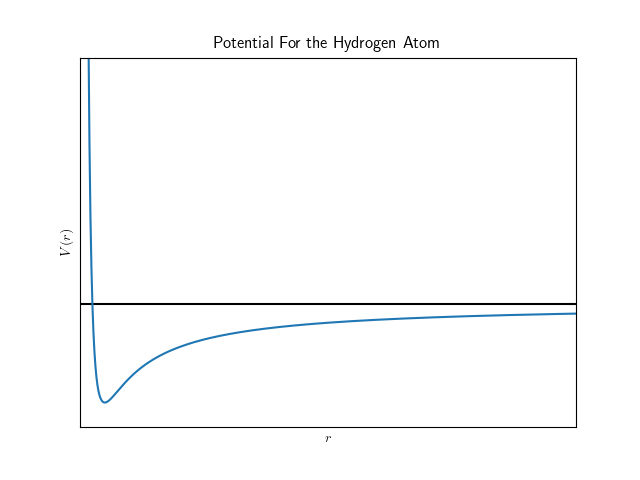
\includegraphics[scale=0.6]{hydrogen_potential.png}
        \caption{The potential for the hydrogen atom.}
        \label{fig:hydrogen atom potential}
    \end{figure}

    To tidy away even more constants we define
    \[a_0 = \frac{\hbar^2}{\mu e^2} \approx \SI{0.52}{\angstrom}, \qquad \text{and} \qquad E_I = \frac{\hbar^2}{2\mu a_0^2} = \frac{\mu e^4}{2\hbar^2} \approx \SI{13.6}{\electronvolt}.\]
    \(a_0\) is called the Bohr radius.
    We will see the physical significance of these values later.
    We now use these quantities to rescale the physical properties of the system:
    \[\rho = \frac{r}{a_0}, \qquad\text{and}\qquad \lambda_\ell = \sqrt{-\frac{E_\ell}{E_I}}.\]
    Note that since \(E_\ell < 0\) for a bound electron \(\lambda\in\reals\).
    We also define \(u_\ell(\rho) = \chi_\ell(\rho)\).
    Using this we have
    \begin{align*}
        -\lambda_\ell^2E_I\chi(a_0\rho) &= -\lambda_\ell^2E_I u_\ell(\rho)\\
        &= \left[-\frac{\hbar^2}{2\mu}\frac{1}{a_0^2}\dv[2]{\rho} + \frac{\hbar^2\ell(\ell + 1)}{2\mu a_0^2\rho^2} - \frac{e^2}{a_0\rho}\right]\chi_\ell(a_0\rho)\\
        &= \left[-\frac{\hbar^2}{2\mu}\frac{1}{a_0^2}\dv[2]{\rho} + \frac{\hbar^2\ell(\ell + 1)}{2\mu a_0^2\rho^2} - \frac{e^2}{a_0\rho}\right]u_\ell(\rho).
    \end{align*}
    Which gives us
    \[\left[-\frac{\hbar^2}{2\mu}\frac{1}{a_0^2}\dv[2]{\rho} + \frac{\hbar^2\ell(\ell + 1)}{2\mu a_0^2\rho^2} - \frac{e^2}{a_0\rho} + \lambda_\ell^2E_I\right]u_\ell(\rho) = 0.\]
    Dividing through by \(-\hbar^2/2\mu a_0^2\) we have
    \[\left[\dv[2]{\rho} - \frac{\ell(\ell + 1)}{\rho^2} + \frac{2\mu a_0e^2}{\hbar^2\rho} - \lambda_\ell^2\frac{2\mu a_0^2E_I}{\hbar^2}\right]u_\ell(\rho) = 0.\]
    Using the definitions of \(a_0\) and \(E_I\) this becomes
    \[\left[\dv[2]{\rho} - \frac{\ell(\ell + 1)}{\rho^2} + \frac{2}{\rho} - \lambda_\ell^2\right]u_\ell(\rho) = 0.\]
    
    \subsubsection{Solution to the Radial Equation}
    To motivate an ansatz we will look at the limiting behaviour of the radial equation.
    First consider the case that \(\rho \to \infty\), in this case the radial equation reduces to
    \[\left[\dv[2]{\rho} - \lambda^2\right]u_\ell(\rho) = 0.\]
    The solutions to this are
    \[u_\ell(\rho) = e^{\pm\lambda_\ell\rho}.\]
    We discard the exponential growth solution as it is non-normalisable so we are left only with the exponential decay solution.
    It makes sense for the radial solution to decay exponentially as it becomes increasingly unlikely for the electron to be found as we move away from the proton.
    We make the ansatz that
    \[u_\ell(\rho) = e^{-\lambda_\ell\rho}\eta_\ell(\rho).\]
    Substituting this into the radial equation we have
    \begin{align*}
        0 &= \dv[2]{\rho}[e^{-\lambda_\ell\rho}\eta_\ell(\rho)] + \left[\frac{2}{\rho} - \frac{\ell(\ell + 1)}{\rho^2} - \lambda_\ell^2\right]e^{-\lambda_\ell\rho}\eta_\ell(\rho)\\
        &= \dv[2]{\eta_\ell}{\rho}e^{-\lambda_\ell\rho} + 2\dv{\eta_\ell}{\rho}\dv{\rho}e^{-\lambda_\ell\rho} + \eta_\ell(\rho)\dv[2]{\rho}e^{-\lambda_\ell\rho} + \left[\frac{2}{\rho} - \frac{\ell(\ell + 1)}{\rho^2} - \lambda_\ell^2\right]e^{-\lambda_\ell\rho}\eta_\ell(\rho)\\
        &= \dv[2]{\eta_\ell}{\rho}e^{-\lambda_\ell\rho} -2\lambda_\ell 2\dv{\eta_\ell}{\rho}e^{-\lambda_\ell} + \lambda_\ell^2\eta_\ell(\rho)e^{-\lambda_\ell\rho} + + \left[\frac{2}{\rho} - \frac{\ell(\ell + 1)}{\rho^2} - \lambda_\ell^2\right]e^{-\lambda_\ell\rho}\eta_\ell(\rho).\\
    \end{align*}
    Dividing through by \(e^{-\lambda_\ell\rho}\) we have
    \begin{equation}\label{eqn:radial eqn in eta}
        \dv[2]{\eta_\ell}{\rho} - 2\lambda_\ell\dv{\eta_\ell}{\rho} +  \left[\frac{2}{\rho} - \frac{\ell(\ell + 1)}{\rho^2}\right]\eta_\ell(\rho) = 0.
    \end{equation}
    
    Now as \(\rho\to 0\) we know from section~\ref{sec:behaviour near the origin central potential} that \(u_\ell(\rho)\sim \rho^{\ell + 1}\).
    We expand \(\eta_\ell\) as a power series in \(\rho\) as
    \[\eta_\ell(\rho) = \rho^{\ell + 1}\sum_{q = 0}^{\infty} c_q\rho^q.\]
    Inserting this into equation~\ref{eqn:radial eqn in eta} we have
    \begin{align*}
        0 &= \sum_q \left[(q + \ell + 1)(q + \ell)c_q\rho^{q + \ell - 1} - 2\lambda_\ell(q + \ell + 1)c_q\rho^{\ell + 1} + 2c_q\rho^{q + \ell} - \ell(\ell + 1)c_q\rho^{q + \ell - 1}\right]\\
        &= \sum_q q(q + 2\ell + 1)c_q\rho^{q + \ell - 1} - \sum_q 2(\lambda_\ell[q + \ell + 1] - 1)c_q\rho^{q + \ell}
        \shortintertext{relabelling, \(q \to q - 1\) in the second sum we have}
        &= \sum_q\left[q(q + 2\ell + 1)c_q - 2[\lambda_\ell(q + \ell) - 1]c_{q-1}\right]\rho^{q + \ell - 1}.
    \end{align*}
    Since we require this to hold for all \(\rho\) we have that for all \(q\)
    \begin{equation}\label{eqn:recursion relation}
        q(q + 2\ell + 1)c_q - 2[\lambda_\ell(q + \ell) - 1]c_{q-1} = 0.
    \end{equation}
    This gives us a recursion relation between the coefficients of the Taylor expansion of \(\eta_\ell(\rho)/\rho^{\ell + 1}\).
    For large \(q\) we have
    \[\frac{c_q}{c_{q-1}} = \frac{2\lambda_\ell(q + 1) - 2}{q(q + 2\ell + 1)} \to \frac{2\lambda}{q}\]
    as \(q \to \infty\) we have
    \[c_q \sim c_{q-1}\frac{2\lambda}{q} \sim \frac{(2\lambda_\ell)^q}{q!}.\]
    This is the asymptotic behaviour that we expect to give exponential growth in a Taylor series so we expect \(\eta_\ell(\rho) \sim \rho^{\ell + 1}e^{2\lambda\rho}\).
    However this is not normalisable.
    The only way for this to be normalisable is if for some \(q = n_r\) we have \(c_{n_r} = 0\) as this means that \(c_q = 0\) for all \(q \ge n_r\).
    This means that \(\eta_\ell\) is a polynomial of order \(n_r\).
    Setting \(q = n_r\) in equation~\ref{eqn:recursion relation} we have that
    \[2[\lambda_{n\ell}(n_r + 1) - 1]c_{n_r-1} = 0 \implies \lambda_{n\ell} = \frac{1}{n_r + \ell} = \frac{1}{n}.\]
    Here we introduce \(n\), the \define{principle quantum number}.
    We see that \(\lambda_{n\ell}\) is quantised as a result of requiring the wave function be normalisable.
    
    \subsubsection{Physical Interpretation}
    Since \(\lambda_{n\ell}\) is quantised the energy is also quantised as
    \[E_{n\ell} = -\frac{E_I}{(n_r + \ell)^2} = -\frac{E_I}{n^2}.\]
    We see that \(E_I\) is the energy needed to remove an electron from the ground state, \(n = 1\).
    That is \(E_I\) is the ionisation energy of hydrogen.
    Going back to the definition of \(E_I\) we can write
    \[E_I = \frac{\mu e^4}{2\hbar^2} = \frac{1}{2}\alpha^2\mu c^2\]
    where
    \[\alpha = \frac{e^2}{\hbar c^2} = \frac{q^2}{4\pi\varepsilon_0\hbar c} \approx \frac{1}{137}\]
    is the \define{fine-structure constant}.
    Notice that \(\mu \approx m_e\) and therefore \(\mu c^2\) is approximately the rest energy of the electron.
    The energy levels are on the scale of \(\alpha^2\mu c^2/2 \approx \mu c^2 \num{2.7e-5}\).
    Since the energy levels are on a scale so much smaller than the rest mass of the electron (which is in turn much less than the rest energy of the proton) we are justified in using a non-relativistic approach.
    Any relativistic corrections will typically be \(\order{\alpha}\).
    Further justification is provided by Heisenberg's uncertainty principle.
    Taking \(a_0\) to be a typical length scale in hydrogen we have that \(\Delta p \approx a_0\hbar/2 = \mu e^2/\hbar\).
    We can also use the symmetry to state that positive and negative momenta are equally likely so \(\Delta p = \sqrt{\expected{p^2} - \expected{p}^2} = \sqrt{\expected{p^2}}\) from which we have
    \[v \sim \frac{p}{\mu} \sim \frac{e^2}{\hbar} = \alpha c \approx \frac{1}{137}c \ll c.\]
    So we see that once again relativity only comes into play on scales less than \(a_0\).
    Any relativistic corrections are going to be on the order of \(\order{v/c} = \order{\alpha}\).
    
    We can write the energy levels further as
    \[E_n = -\frac{e^2}{2n^2a_0} = -\frac{\mu e^4}{2n^2\hbar^2} = -\frac{\mu q^4}{32\hbar^2\pi^2\varepsilon_0^2n^2}.\]
    From \(n = n_r + \ell\) since \(n, n_r\in\naturals_{>0}\) we have that \(\ell = 0, 1, \dotsc, n - 1\), which corresponds to \(n_r = n, n-1, \dotsc, 1\).
    For a particular value of \(\ell\) we have \((2\ell + 1)\)-fold degeneracy.
    This means that the total degeneracy of the eigenvalue \(E_n\) is
    \[g_n = \sum_{\ell = 0}^{n - 1}(2\ell + 1) = 2\sum_{\ell=0}^{n-1}\ell + \sum_{\ell=0}^{n-1}1 = (n - 1)n + n = n^2.\]
    Here we have used the result proven in section~\ref{sec:proof sum 0 to n of r is 0.5 n(n+1)}.
    The fact that \(E_n = E_I/n^2\) was first proposed by Niels Bohr in 1913 before the full quantum picture that we have seen here was known.
    However quantum mechanics is still needed to find the degeneracy of \(E_n\) and other important properties.
    
    The full radial wave function is
    \[R_{n\ell}(r) = \frac{\chi_{n\ell}(r)}{r} = \frac{u_{n\ell}(a_0\rho)}{a_0\rho} = \frac{1}{a_0\rho}e^{-\lambda\rho}\eta_{n\ell}(\rho) = \frac{1}{a_0\rho}e^{-\lambda\rho}\sum_{q=0}^{n_r} c_q\rho^{q + \ell + 1}.\]
    The polynomials in the last term are called the \define{associated Laguerre polynomials}.
    They can be looked up in standard texts.
    If we do this we find that
    \begin{align*}
        R_{1,0}(r) &= \frac{2}{a^{3/2}}e^{-r/a_0}\\
        R_{2,0}(r) &= \frac{1}{2\sqrt{2}} \frac{1}{a^{3/2}} \left[2 - \frac{r}{a_0}\right] e^{-r/(2a_0)}\\
        R_{2,1}(r) &= \frac{1}{2\sqrt{6}} \frac{1}{a^{3/2}} \frac{r}{a_0} e^{-r/(2a_0)}.
    \end{align*}
    Notice that \(R\sim a_0^{-3/2}\) so \(\abs{R}^2\sim a_0^3\).
    This means that \(\abs{R}\) has units of probability per unit volume, which is what we want since \(\psi = RY_\ell^m\) is a probability density and \(Y_\ell^m\) is dimensionless.
    
    \section{Non-degenerate Time-Independent Perturbation Theory}
    Many problems in quantum mechanics involve solving the \gls{tise}.
    In most cases however an analytic solution does not exist.
    If this is the case then the best we can do is find an estimate.
    One of the most common ways to do this is perturbation theory.
    This gives us a way to solve the \gls{tise} for a system with a Hamiltonian of the form
    \[\operator{H} = \operator{H}_0 + \varepsilon\operator{V}.\]
    Here \(\operator{H}\) is the Hamiltonian we wish to find a solution for, \(\operator{H}_0\) is a Hamiltonian for which we know the solution to the \gls{tise} and \(\operator{V}\) is known as a perturbation.
    We will assume that \(\operator{H}\) and \(\operator{H}_0\) have discrete, non-degenerate eigenvalues.
    Let \(\ket{\varphi_n}\) be the eigenstate of \(\operator{H}_0\) with eigenvalue \(E_n^{(0)}\), i.e.
    \[\operator{H}_0\ket{\varphi_n} = E_n^{(0)}\ket{\varphi_n}.\]
    We want to find \(\ket{\psi_n}\) and \(E_n\) such that
    \[\operator{H}\ket{\psi_n} = E_n\ket{\psi_n}.\]
    We look for a solution expanded in terms of \(\varepsilon\).
    We can expand the energy as
    \[E_n = E_{0n} + \varepsilon E_{1n} + \varepsilon^2E_{2n} + \order{\varepsilon^3} = \sum_{k=1}^{\infty} \varepsilon^kE_{kn},\]
    where \(E_{kn}\) are to be found.
    Similarly we can expand the eigenstate as
    \[\ket{\psi_n} = \ket{\psi_{0n}} + \varepsilon\ket{\psi_{1n}} + \varepsilon^2\ket{\psi_{2n}} + \order{\varepsilon^3} = \sum_{k=1}^{\infty} \varepsilon^k\ket{\psi_{kn}},\]
    where \(\ket{\psi_{kn}}\) are to be found.
    Inserting these expansions and the definition of \(\operator{H}\) into the \gls{tise} we find that
    \[(\operator{H}_0 + \varepsilon\operator{V})\sum_{i=1}^{\infty}\ket{\psi_{in}} = \left[\sum_{j=1}^{\infty}E_{jn}\right]\left[\sum_{k=1}^{\infty}\ket{\psi_{kn}}\right].\]
    Expanding these sums up to second order in \(\varepsilon\) we have
    \begin{multline*}
        \operator{H}_0\ket{\psi_{0n}} + \varepsilon(\operator{H}_0\ket{\psi_{1n}} + \operator{V}\ket{\psi_{0n}}) + \varepsilon^2(\operator{H}_0\ket{\psi_{2n}} + \operator{V}\ket{\psi_{1n}}) + \order{\varepsilon^3} =\\
        E_{0n}\ket{\psi_{0n}} + \varepsilon(E_{0n}\ket{\psi_{1n}} + E_{1n}\ket{\psi_{0n}}) + \varepsilon^2(E_{0n}\ket{\psi_{2n}} + E_{1n}\ket{\psi_{1n}} + E_{2n}\ket{\psi_{0n}}) + \order{\varepsilon^3}.
    \end{multline*}
    \subsection{Zeroth Order}
    Equating coefficients of terms of zeroth order in \(\varepsilon\) we have
    \[\operator{H}_0\ket{\psi_{0n}} = E_{0n}\ket{\psi_{0n}}.\]
    Notice that this is exactly what we would get if \(\varepsilon = 0\) so this is just the unperturbed Hamiltonian meaning that \(\ket{\psi_{0n}} = \ket{\varphi_n}\) and \(E_{0n} = E_n^{(0)}\).
    
    \subsection{First Order}
    \subsubsection{Energy Perturbation}
    Equating coefficients of terms of first order in \(\varepsilon\) we have
    \[\operator{H}_0\ket{\psi_{1n}} + \operator{V}\ket{\psi_{0n}} = E_{0n}\ket{\psi_{1n}} + E_{1n}\ket{\psi_{0n}}.\]
    Rearranging this we have
    \begin{equation}\label{eqn:perturbation theory first order terms}
        (\operator{H} - E_{0n})\ket{\psi_{1n}} - (\operator{V} - E_{1n})\ket{\psi_{0n}} = 0.
    \end{equation}
    We then take an inner product with \(\ket{\psi_{0n}}\):
    \[\bra{\psi_{0n}}\operator{H}_0\ket{\psi_{1n}} - E_{0n}\braket{\psi_{0n}}{\psi_{1n}} - \bra{\psi_{0n}}\operator{V}\ket{\psi_{0n}} + E_{1n}\braket{\psi_{0n}}{\psi_{0n}} = 0.\]
    Consider the first term of this sum:
    \begin{align*}
        \bra{\psi_{0n}}\operator{H}_0\ket{\psi_{1n}} &= (\bra{\psi_{1n}}\operator{H}_0\hermit\ket{\psi_{0n}})^*\\
        &= (\bra{\psi_{1n}}\operator{H}_0\ket{\psi_{0n}})^*\\
        &= E_{0n}(\braket{\psi_{1n}}{\psi_{0n}})^*\\
        &= E_{0n}\braket{\psi_{0n}}{\psi_{1n}}.
    \end{align*}
    So the first term cancels with the second, note that we make no assumptions about \(\ket{\psi_{kn}}\) being orthonormal.
    Rearranging the remaining two terms we have
    \[E_{1n} = \frac{\bra{\psi_{0n}}\operator{V}\ket{\psi_{0n}}}{\braket{\psi_{0n}}{\psi_{0n}}} = \frac{\bra{\varphi_n}\operator{V}\ket{\varphi_n}}{\braket{\varphi_n}{\varphi_n}} = V_{00},\]
    where \(V\) is a matrix representation of \(\operator{V}\) and we assume that \(\ket{\psi_n}\) are orthonormal.
    Note that since \(E_{0n}\) is a shift in the energy to first order it is sometimes written as \(\Delta E_{0n}\).
    
    \subsubsection{Eigenstate Perturbation}
    We can express \(\ket{\psi_{1n}}\) in the energy eigenbasis of \(\operator{H}_0\):
    \[\ket{\psi_{1n}} = \sum_{m}c_m\ket{\varphi_m},\]
    where as usual \(c_m = \braket{\varphi_m}{\psi_{1n}}\).
    We can take a scalar product of equation~\ref{eqn:perturbation theory first order terms} with \(\ket{\varphi_m}\) and we get
    \[\bra{\varphi_m}\operator{H}_0\ket{\psi_{1n}} - E_{0n}\braket{\varphi_m}{\psi_{1n}} + \bra{\varphi_m}\operator{V}\ket{\varphi_n} + E_{1n}\braket{\varphi_m}{\varphi_n} = 0.\]
    We will first consider the case when \(m \ne n\), thus the last term is zero.
    Analogously to how we worked with the first term for the energy perturbation we can show that the first term is simply \(E_{0m}\braket{\varphi_m}{\psi_{1n}}\).
    Thus
    \[(E_{0m} - E_{0n})\braket{\varphi_m}{\psi_{1n}} + \bra{\varphi_m}\operator{V}\ket{\varphi_n}.\]
    Hence
    \[c_m = \braket{\varphi_m}{\psi_{1n}} = \frac{\bra{\varphi_m}\operator{V}\ket{\varphi_n}}{E_{0n} - E_{0m}} = \frac{V_{mn}}{E_{0n - E_0m}}.\]
    Note that \(E_{0n} = E_n^{(0)}\) and \(E_{0m} = E_m^{(0)}\) are simply the \(n\)th and \(m\)th energy eigenvalues of \(\operator{H}_0\) so are known quantities.
    Knowing this we can express the \(n\)th perturbed eigenstate, \(\ket{\psi_{n}}\), as
    \[\ket{\psi_{n}} = \ket{\varphi_n} + \varepsilon\sum_{m\ne n}\frac{V_{mn}}{E_{0n} - E_{0m}}\ket{\varphi_m} + \varepsilon c_n\ket{\varphi_n} + \order{\varepsilon^2}.\]
    So to find the adjustment needed at first order we just need to compute \(c_n\) which we can do by imposing normalisation, taking the inner product of this with \(\ket{\psi_{n}}\) we have
    \[1 = \braket{\psi_{n}}{\psi_{n}} = 1 + 2\varepsilon c_n\braket{\varphi_n}{\varphi_n} + \order{\varepsilon^2},\]
    where we have used the fact that \(\ket{\varphi_n}\) are orthonormal so \(\braket{\varphi_n}{\varphi_m} = \delta_{nm}\) meaning that the inner product with the sum term gives zero as \(\ket{\varphi_n}\) is explicitly excluded from that sum.
    From this we conclude that we must have \(c_n = 0\), so \(\ket{\psi_{1n}}\) has no component in the \(\ket{\varphi_n}\) direction.
    Thus
    \[\ket{\psi_{1n}} = \sum_{m\ne n} \frac{V_{mn}}{E_{0n} - E_{0m}}\ket{\varphi_m}.\]
    
    \subsection{Second Order}
    Equating coefficients of terms of second order in \(\varepsilon\) we have
    \[\operator{H}_0\ket{\psi_{2n}} + \operator{V}\ket{\psi_{1n}} = E_{0n}\ket{\psi_{2n}} + E_{1n}\ket{\psi_{1n}} + E_{2n}\ket{\psi_{0n}}.\]
    Rearranging this we have
    \[(\operator{H}_0 - E_{0n})\ket{\psi_{2n}} + (\operator{V} - E_{1n})\ket{\psi_{1n}} - E_{2n}\ket{\psi_{0n}} = 0.\]
    We then take the inner product with \(\ket{\varphi_n}\) and we have
    \[\bra{\varphi_n}\operator{H}_{0}\ket{\psi_{2n}} - E_{0n}\braket{\varphi_n}{\psi_{2n}} + \bra{\varphi_n}\operator{V}\ket{\psi_{1n}} - E_{1n}\braket{\varphi_n}{\psi_{1n}} - E_{2n}\braket{\varphi_n}{\psi_{0n}} = 0.\]
    The first term is equal to \(E_{0n}\braket{\varphi_n}{\psi_{2n}}\) so combines with the second term to give zero.
    The fourth term is zero as \(\ket{\psi_{1n}}\) has no \(\ket{\varphi_n}\) component.
    The scalar product in the fifth term is simply one as \(\ket{\psi_{0n}} = \ket{\varphi_n}\).
    Thus
    \begin{align*}
        E_{2n} &= \bra{\varphi_n}\operator{V}\ket{\psi_{1n}}\\
        &= \bra{\varphi_n}\operator{V}\sum_{m\ne n} \frac{V_{mn}}{E_{0n} - E_{0m}}\ket{\varphi_m}\\
        &= \sum_{m\ne n}\frac{V_{mn}}{E_{0n} - E_{0m}}\bra{\varphi_n} \operator{V}\ket{\varphi_m}\\
        &= \sum_{m\ne n}\frac{V_{mn}V_{nm}}{E_{0n} - E_{0m}}\\
        &= \sum_{m\ne n}\frac{\abs{V_{mn}^2}}{E_{0n} - E_{0m}}.
    \end{align*}

    \subsection{Perturbation Examples}
    \subsubsection{Infinite Well With a Cosine Floor}
    Consider the potential
    \[
        V(x) = 
        \begin{cases}
            V_0\cos\left(\frac{\pi x}{2a}\right), & \abs{x} \le a,\\
            \infty, & \abs{x} > a.
        \end{cases}
    \]
    If we define \(\operator{H}'\) as
    \[V_0 \cos\left(\frac{\pi x}{2a}\right)\]
    then we can view the Hamiltonian for this system as
    \[\operator{H} = \operator{H}_0 + \operator{H}'\]
    where \(\operator{H}_0\) is the Hamiltonian for an infinite square well.
    The solution to the \gls{tise} for the infinite square well is discussed in section~\ref{sec:infinite square well}.
    In particular the \(n\)th energy level is
    \[E_n^{(0)} = \frac{\hbar^2\pi^2 n^2}{8ma^2},\]
    and the corresponding eigenfunction is
    \[
        \varphi_{(n)}(x) =
        \begin{cases}
            \frac{1}{\sqrt{a}}\cos\left(\frac{n\pi x}{2a}\right), & \text{for odd}~n,\\
            \frac{1}{\sqrt{a}}\sin\left(\frac{n\pi x}{2a}\right), & \text{for even}~n.
        \end{cases}
    \]
    Perturbation theory only gives a good estimate if the energy shift due to the addition of \(\operator{H}'\) to the Hamiltonian is small, in this case this means that we require \(V_0 \ll E_0^{(2)} - E_0^{(1)}\).
    The energy shift is then
    \begin{align*}
        \Delta E_1 &= \bra{\varphi^{(1)}}\operator{H}'\ket{\varphi^{(1)}}\\
        &= \int_{-a}^{a} \varphi^{(1)}(x)^*V_0\cos\left(\frac{\pi x}{2a}\right)\varphi^{(1)} (x)\dd{x}\\
        &= \frac{V_0}{a} \int_{-a}^{a} \cos^3\left(\frac{\pi x}{2a}\right) \dd{x}\\
        &= \frac{8V_0}{3\pi}.
    \end{align*}
    So to first order the energy of the ground state is
    \[E_1 = E_1^{(0)} + \Delta E_1 = \frac{\hbar^2\pi^2 n^2}{8ma^2} + \frac{8V_0}{3\pi}.\]
    
    \subsubsection{Helium}
    Helium is a two electron atom.
    If we ignore the interaction between the electrons then the Hamiltonian for a helium atom is
    \[\operator{H}_0 = \frac{\hbar^2}{2m}\laplacian_1 - \frac{Ze^2}{r_1} + \frac{\hbar^2}{2m}\laplacian_2 - \frac{Ze^2}{r_2} = \operator{H}_0^{(1)} + \operator{H}_0^{(2)}.\]
    Here \(m\) is the reduced mass of an electron and the nucleus,
    \[\frac{1}{m} = \frac{1}{m_e} + \frac{1}{2m_p} \approx \frac{1}{m_e}.\]
    The distances \(r_1\) and \(r_2\) are the distances from the nucleus to the relevant electron, where we model the four nucleon nucleus as a point charge of charge \(Z = 2e\).
    The Laplacian operator, \(\laplacian_1\) or \(\laplacian_2\), acts only on the coordinates of the relevant electron.
    
    The Hamiltonian is independent of the spin of any one part of the system.
    This means that we can treat the spin of the electrons as we do for a normal two particle, spin 1, system.
    A generic state, \(\ket{\Psi}\in \hilbert\) can be described by \(\ket{\psi}\in\hilbert_{\text{space}}\) and \(\ket{s, s_z}\in\hilbert_{\text{spin}}\) as
    \[\ket{\Psi} = \ket{\psi} \tensorProd \ket{s, s_z} = \ket{\psi; s, s_z}.\]
    As discussed in section~\ref{sec:total angular momentum}
    \[\ket{s=1, s_z=1} = \ket{\spinUp\spinUp}, \qquad \ket{s=1, s_z=-1} = \ket{\spinDown\spinDown}, \qquad\ket{s=1, s_z=0} = \frac{\sqrt{2}}{2}(\ket{\spinUp\spinDown} + \ket{\spinDown\spinUp}),\]
    \[\text{and}\qquad \ket{s=0, s_z=0} = \frac{\sqrt{2}}{2}(\ket{\spinUp\spinDown} - \ket{\spinDown\spinUp}).\]
    The spatial wave function is given by
    \[\braket{\vv{r_1}, \vv{r_2}}{\psi} = \psi(\vv{r_1}, \vv{r_2}) = \psi^{(1)}(\vv{r_1})\psi^{(2)}(\vv{r_2}),\]
    where we assume in the last step that a separable solution exists.
    Each \(\psi^{(k)}\) must satisfy the \gls{tise} for the relevant Hamiltonian:
    \[\operator{H}_0^{(k)}\psi^{(k)}(\vv{r_k}) = \left[\frac{\hbar^2}{2m}\laplacian_k - \frac{Ze^2}{r_k}\right]\psi^{(k)}(\vv{r_k}) = E^{(k)}\psi^{(k)}(\vv{r_k}).\]
    This is simply the \gls{tise} that we solved for the hydrogen atom but with the nucleus charge changed to \(Z = 2e\) instead of \(Z = e\).
    The solutions to this are the states \(u_{n\ell m}\), where the ground state is
    \[\psi^{(k)}(\vv{r_k}) = u_{100}(\vv{r_k}) = \frac{1}{\sqrt{\pi}} \left(\frac{Z}{a_0}\right)^{3/2}e^{-r/a_0}.\]
    Thus
    \[\braket{\vv{r_1}, \vv{r_2}}{\Psi} = u_{100}(\vv{r_1})u_{100}(\vv{r_2})\sum_{\alpha = 1}^{4}c_\alpha\ket{\alpha}\]
    where
    \[\{\ket{\alpha}\} = \{\ket{s, s_z}\st s = 0, 1~\text{and}~s_z = -s, \dotsc, s\}.\]
    Electrons are fermions.
    This means that \(\ket{\Psi}\) should be antisymmetric under exchanging of 1 and 2.
    The radial part, \(u_{100}(\vv{r_1})u_{100}(\vv{r_2})\), is symmetric under exchanging of 1 and 2 so the spin part must be antisymmetric.
    The only antisymmetric spin state available is \(\ket{s = 0, s_z = 0}\).
    
    We are now in a position to consider what happens when we include the interaction between the electrons.
    This interaction is characterised by the potential
    \[\operator{V} = \frac{e^2}{\abs{\vv{r_1} - \vv{r_2}}}.\]
    The energy shift due to this perturbation is
    \begin{align*}
        \Delta E_1 &= \bra{\Psi}\operator{V}\ket{\Psi}\\
        &= \bra{\psi; 0, 0}\operator{V}\ket{\psi; 0, 0}
        \shortintertext{using the fact that \(\operator{V}\) acts only on the radial part this becomes}
        &= \braket{0, 0}{0, 0}\bra{\psi}\operator{V}\ket{\psi}
        \shortintertext{considering the ground state, \(\psi(\vv{r}) = u_{100}(\vv{r})\), or equivalently \(\ket{\psi} = \ket{100}\), this becomes}
        &= \bra{100, 100}\operator{V}\ket{100, 100}\\
        &= \int \dd[3]{r_1}\dd[3]{r_2} u_{100}^*(\vv{r_1})u_{100}^*(\vv{r_2})\frac{e^2}{\abs{\vv{r_1} - \vv{r_2}}}u_{100}(\vv{r_1})u_{100}(\vv{r_2})\\
        &= \left(\frac{eZ^3}{\pi a_0^3}\right)^2 \int \dd[3]{r_1}\dd[3]{r_2} \exp\left(-\frac{2Z(r_1 + r_2)}{a_0}\right)\frac{1}{\abs{\vv{r_1} - \vv{r_2}}}\\
        &= \frac{5}{4}ZE_I
    \end{align*}
    where \(E_I \approx \SI{13.6}{\electronvolt}\) is defined as it was in section~\ref{sec:stationary states hydrogen atom}.
%    \clearpage
%    \appendix
%    \part*{Appendix}
%    \addcontentsline{toc}{part}{Appendix}
%    \begingroup
%    \let\clearpage\relax
%            \section{Sets and Logic}
        \subsection{Sets}
        A set is a collection of objects, say the objects \(\square\), \(\dagger\), and \(\star\).
        To denote a set containing all of these objects and nothing else we write \(\mathcal{A} = \{\square, \dagger, \star\}\), here `\(\mathcal{A}\)' is just a name that we give the set, in the same way we may say \(x = 2\).
        Sets may contain an infinite number of objects, for example the rational numbers, \(\rationals\), is a set of all fractions of the form \(a/b\) with \(a\) and \(b \ne 0\) being integers.
        The objects in a set are called its elements.
        It is also possible for a set to have no members, in which case we denote this set \(\emptyset\).
        We denote an element being in a set with \(\in\).
        For example we might write \(\square \in \mathcal{A}\) which we read as `\(\square\) is in the set \(\mathcal{A}\)', or \(\pi \in \reals\) which is read as '\(\pi\) is in the set of real numbers' or more commonly as `\(\pi\) is a real number'.
        We denote an element \emph{not} being in a set with \(\notin\), for example \(\diamondsuit \notin \mathcal{A}\) or \(e\notin\rationals\).
        
        Two sets are equal if and only if every element in one set is in the other set and vice versa.
        Note that their is no mention of the order of the elements or how many times an element is included as long as it is included at least one in each set.
        Therefore the following is a true statement:
        \[\mathcal{A} = \{\square, \dagger, \star\} = \{\dagger, \star, \square\} = \{\dagger, \square, \star, \square, \star, \star\}.\]
        Note also that by this definition of equality there is only one empty set, \(\emptyset\).
        It doesn't matter what is not in the set, equality is defined based on what is in the set so if there is nothing in the set then the set is the empty set.
        
        Set builder notation is a way of defining sets where simply listing all of the elements in the set is impractical.
        A set in set builder notation looks like
        \[\mathcal{B} = \{\text{a} \in \mathcal{A} \st \text{condition on }a\}.\]
        Here \(\mathcal{A}\) is some underlying set.
        \(\mathcal{B}\) is composed of elements in \(\mathcal{A}\) such that the given condition on \(a\) is true.
        For example the even numbers could be written as
        \[\{n\in\integers \st n\equiv 0\pmod{2}\}\]
        where \(n \equiv 0 \pmod{2}\) means that \(n/2\) has a remainder of 0.
        
        Two commonly defined operations between set are unions and intersections.
        The union between two sets, \(\mathcal{A}\) and \(\mathcal{B}\) is
        \[\mathcal{A} \union \mathcal{B} = \{a\st a\in\mathcal{A}\;\text{or}\;a\in\mathcal{B}\}.\]
        That is the set of all elements, \(a\), that are in either one of the two sets \(\mathcal{A}\) or \(\mathcal{B}\) (or both sets).
        The intersection between two sets, \(\mathcal{A}\) and \(\mathcal{B}\) is
        \[\mathcal{A} \intersection \mathcal{B} = \{a\st a\in \mathcal{A}\;\text{and}\;\mathcal{B}\}.\]
        That is the set of all elements that are in both of the sets, \(\mathcal{A}\) and \(\mathcal{B}\).
        
        The use of sets in probability is as collections of possible outcomes.
        For example if we are rolling a normal six sided die then the set of all possible outcomes is
        \[\mathcal{S} = {1, 2, 3, 4, 5, 6}\]
        This is the sample space, it is the set of all possible outcomes.
        Suppose we ask the question `what is the chance of rolling an odd prime number'?
        There are two conditions here `odd' and `prime'.
        The set of all odd numbers that are in \(\mathcal{S}\) is
        \[\mathcal{O} = {1, 3, 5}.\]
        The set of all prime numbers in \(\mathcal{S}\) is
        \[\mathcal{P} = {2, 3, 5}.\]
        The set of all odd prime numbers in \(\mathcal{S}\) is then
        \[\mathcal{O} \intersection \mathcal{P} = \{1, 3, 5\} \intersection \{2, 3, 5\} = \{3, 5\}.\]
        Thus we see there are 2 odd primes out of 6 possibilities so the probability of rolling an odd prime is \(2/6 = 1/3\).
        We could ask the similar question `what is the probability of rolling a number that is either odd, prime, or both'?
        The set of all numbers that are odd, prime, or both is
        \[\mathcal{O} \union \mathcal{P} = \{1, 3, 5\} \union \{2, 3, 5\} = \{1, 2, 3, 5\}.\]
        Thus there are 4 numbers that are odd or prime and the chance that rolling the die results in one of these numbers is \(4/6 = 2/3\).
        
        With a frequentist view of probability we see that `and' questions reduce to intersections of sets of possible values whereas `or' questions reduce to unions of sets of possible values.
        This reflects the `and' and `or' in the definitions of intersections and unions.
        
        \subsection{Logic}
        In boolean logic a statement is something that takes one of two values, true, denoted 1, or false, denoted 0.
        We can define various operations on these statements.
        Let \(\mathscr{A}\) and \(\mathscr{B}\) be statements.
        Then we define conjunction, \(\conjunction\), by the following table:
        \[
            \begin{array}{cc|c}
                \mathscr{A} & \mathscr{B} & \mathscr{A} \conjunction \mathscr{B}\\\hline
                1 & 1 & 1\\
                1 & 0 & 0\\
                0 & 1 & 0\\
                0 & 0 & 0
            \end{array}
        \]
        That is \(\mathscr{A}\conjunction\mathscr{B}\) is true only if both \(\mathscr{A}\) and \(\mathscr{B}\) are true.
        We define disjunction, \(\disjunction\), by the following table:
        \[
            \begin{array}{cc|c}
                \mathscr{A} & \mathscr{B} & \mathscr{A} \disjunction \mathscr{B}\\\hline
                1 & 1 & 1\\
                1 & 0 & 1\\
                0 & 1 & 1\\
                0 & 0 & 0
            \end{array}
        \]
        That is \(\mathscr{A}\disjunction\mathscr{B}\) is true so long as at least one of \(\mathscr{A}\) or \(\mathscr{B}\) is true.
        
        We return to rolling a 6 sided die.
        We now use a Bayesian view of probability where we look at confidence in particular statements being true.
        If \(\mathscr{O}\) is the statement `is odd' and \(\mathscr{P}\) is the statement `is prime' then the statement `is odd and prime' is \(\mathscr{O}\conjunction\mathscr{P}\).
        Similarly the statement `is odd or prime' is \(\mathscr{O}\disjunction\mathscr{P}\).
        
        \subsection{Sets and Logic}
        Note the similarity between this notation and the set notation, in particular compare \(\union\)/\(\intersection\) too \(\disjunction\)/\(\conjunction\).
        Also note how the statements \(\mathcal{O}\union\mathcal{P}\)/\(\mathcal{O}\intersection\mathcal{P}\) are the answers too the same questions as \(\mathscr{O}\disjunction\mathscr{P}\)/\(\mathscr{O}\conjunction\mathscr{P}\).
        The reason for this similarity in notation is that (at least when it comes to probability) these two ideas are really equivalent but viewed from a frequentist and Bayesian perspective respectively.
        
        In this work we take both a frequentist and Bayesian view of probability, using whichever better suits our needs.
        For this reason we choose notation that is distinct from both of these.
        If \(A\) and \(B\) are outcomes of some trial then we combine them as
        \[A\logicalAnd B = A, B \iff \mathcal{A} \intersection \mathcal{B} \iff \mathscr{A} \conjunction \mathscr{B},\]
        and
        \[A \logicalOr B \iff \mathcal{A} \union \mathcal{B} \iff \mathscr{A} \disjunction \mathscr{B}.\]
        Here \(\mathcal{A}/\mathcal{B}\) and \(\mathscr{A}/\mathscr{B}\) are the frequentist and Bayesian versions respectively of \(A/B\).
%    \section{Size of a Union}
        Suppose that \(A_i\) are sets for some \(i\in {1, \dotsc, n}\).
        Let
        \[\bigunion_{i = 1}^{n} A_i = A_1 \union A_2 \union \dotsb \union A_n = \{a\st a\in A_1\logicalOr A\in A_2\logicalOr\dotsb\logicalOr a\in A_n\}.\]
        It is useful to know what the size of this union is as it often occurs in probability.
        For example
        \[P(A_1\logicalOr A_2\logicalOr \dotsb \logicalOr A_n) = \frac{1}{|S|}\abs{\bigunion_{i = 1}^n A_i}.\]
        We have already seen that in the case \(n = 2\) we have \(|A_1\union A_2| = |A| + |B| - |A\intersection B|\).
        We arrived at this result by counting the elements in each set and then subtracting the elements that we double counted due to them being counted in both sets.
        We can actually be a little bit more rigorous than this with the following theorem\cite[liebeck].
        \begin{theorem}
            Let \(A\) and \(B\) be finite sets.
            Then
            \[|A \union B| = |A| + |B| - |A\intersection B|\]
        \end{theorem}
        \begin{proof}
            Let \(|A\intersection B| = k\).
            Then \(A\union B = \{x_1, \dotsc, x_k\}\).
            These elements, and no others, are in both \(A\) and \(B\) so we have
            \[A = \{x_1, \dotsc, x_k, a_1, \dotsc, a_l\},\qquad\text{and}\qquad B = \{x_1, \dotsc, x_k, b_1, \dotsc, b_m\}\]
            where \(a_i\) and \(b_i\) are all distinct from each other and \(a_i\notin B\) and \(b_i\notin A\) for all \(i\).
            Then clearly \(|A| = k + l\) and \(|B| = k + m\).
            Now we compute the union
            \[A \union B = \{x_1, \dotsc, x_k, a_1, \dotsc, a_l, b_1, \dotsc, b_m\}.\]
            All of these elements are different so
            \begin{align*}
                |A\union B| &= k + l + m\\
                &= (k + l) + (k + m) - k\\
                &= |A| + |B| - |A\intersection B|.
            \end{align*}
        \end{proof}
        That's all well and good for two sets but what about a finite number of finite sets, \(A_i\)?
        We can use another theorem\cite{liebeck}.
        \begin{theorem}
            Let \(n\) be a positive integer, and  let \(A_1, \dotsc, A_n\) be finite sets.
            Then
            \[\abs{\bigunion_{i = 1}^n A_i} = |A_1 \union \dotsb \union A_n| = c_1 - c_2 + c_3 - \dotsb + (-1)^nc_n\]
            where for \(1 \le i \le n\) the number \(c_i\) is the sum of the sizes of the intersections of the sets taken \(i\) at a time.
            For example if \(n = 3\) then
            \begin{align*}
                c_1 &= |A_1| + |A_2| + |A_3|\\
                c_2 &= |A_1 \intersection A_2| + |A_1 \intersection A_3| + |A_2 \intersection A_3|\\
                c_3 &= |A_1 \intersection A_2 \intersection A_3|.
            \end{align*}
        \end{theorem}
        \begin{proof}
            Let \(x \in \bigunion_{i = 1}^n A_i.\)
            We will show that \(x\) contributes exactly once to the expression we have for the size of this union.
            Suppose that \(x\) belongs to precisely \(k\) of the sets \(A_1, \dotsc, A_n\) where \(1 \le k \le n\).
            Then \(x\) contributes \(k\) to the sum 
            \[c_1 = \sum_{1\le i\le n}|A_i|.\]
            \(x\) also contributes to each term of
            \[c_2 = \sum_{1\le i<j \le n}|A_i\intersection A_j|\]
            in which \(A_i\) and \(A_j\) are among the \(k\) sets which contain \(x\).
            There are \({k\choose 2}\) such terms.
            Similarly \(x\) contributes \({k\choose 3}\) to the sum \(c_3\).
            In general \(x\) contributes \({k\choose i}\) to the sum \(c_i\).
            Therefore the total contribution of \(x\) to our expression is
            \[k - {k\choose 2} + {k\choose 3} - \dotsb + (-1)^{k-1}{k\choose k}.\]
            This happens to be 1.
            Hence each element \(x \in A_1\union\dotsb\union A_n\) contributes exactly once to the expression so we find that
            \[\abs{\bigunion_{i = 1}^n A_i} = |A_1 \union \dotsb \union A_n| = c_1 - c_2 + c_3 - \dotsb + (-1)^nc_n.\]
        \end{proof}
%    \section{Clebsch--Gordan Coefficients}
    The Clebsch--Gordan coefficients are, using the notation of section~\ref{sec:addition of angular momenta}, the coefficients
    \[\braket{j_1, m_1, j_2, m_2}{j, m; j_1, j_2}\]
    in the transformation from the uncoupled to coupled basis:
    \[\ket{j, m; j_1, j_2} = \sum_{m_1 = -j_1}^{j_1}\sum_{m_2 = -j_2}^{j_2} \braket{j_1, m_1, j_2, m_2}{j, m; j_1, j_2} \ket{j_1, m_1, j_2, m_2}.\]
    There is an explicit solution to this, namely
    \begin{align*}
        \braket{j_1, m_1, j_2, m_2}{j, m; j_1, j_2} &= \delta_{m,m_1+m_2} \sqrt{\frac{(2j + 1)(j + j_1 - j_2)!(j - j_1 + j_2)!(j_1 + j_2 - j)!}{(j_1 + j_2 + j + 1)!}} \times\\
        &\qquad \sqrt{(j + m)!(j - m)!(j_1 - m_1)!(j_1 + m_1)!(j_2 - m_2)!(j_2 + m_2)!} \times\\
        &\qquad \sum_k \left[\sqrt{\frac{(-1)^k}{k!(j_1 + j_2 - j - k)!(j_1 - m_1 - k)!(j_2 + m_2 - k)!}}\right.\times\\
        &\qquad\qquad \left.\sqrt{\frac{1}{(j - j_2 + m_1 + k)!(j - j_1 - m_2 + k)!}}\,\,\right].
    \end{align*}
    The summation is over all \(k\in\integers\) such that the argument of every factorial is non-negative.
    Solutions with \(m < 0\) or \(j_1 < j_2\) have been omitted.
    Solutions with \(m < 0\) can be found using the relation
    \[\braket{j_1, m_1, j_2, m_2}{j, m; j_1, j_2} = (-1)^{j - j_1 - j_2}\braket{j_1, m_2, j_2, m_2}{j, -m, j_1, j_2}\]
    and solutions with \(j_1 < j_2\) can be found using the relation
    \[\braket{j_1, m_1, j_2, m_2}{j, m; j_1, j_2} = (-1)^{j - j_1 - j_2}\braket{j_2, m_2, j_1, m_2}{j, m; j_2, j_1}.\]
    
    Clearly this is impractical to use every time.
    The common thing to do is to pre-calculate values or use a computer.
    Some pre-calculated values are given here.
    \subsection{Pre-Calculated Clebsch--Gordan Coefficients}
    When \(j_2 = 0\)  the Clebsch--Gordan coefficients are given by \(\delta_{jj_1}\delta_{mm_1}\).
    
    \begin{table}[ht]
        \centering
        \begin{subtable}{0.25\textwidth}
            \centering
            \begin{tabular}{|l|l|}\hline
                \backslashbox{\(m_1, m_2\)}{\(j\)} & 1\\ \hline
                \(1/2, 1/2\) & 1\\ \hline
            \end{tabular}
            \subcaption{\(m = 1\)}
        \end{subtable}
        \begin{subtable}{0.25\textwidth}
            \centering
            \begin{tabular}{|l|l|}\hline
                \backslashbox{\(m_1, m_2\)}{\(j\)} & 1\\ \hline
                \(-1/2, -1/2\) & 1\\ \hline
            \end{tabular}
            \subcaption{\(m = -1\)}
        \end{subtable}
        \begin{subtable}{0.4\textwidth}
            \centering
            \begin{tabular}{|l|l|l|}\hline
                \backslashbox{\(m_1, m_2\)}{\(j\)} & 1 & 0\\ \hline
                &&\\[-1em]
                \(1/2, -1/2\) & \(\sqrt{1/2}\) & \(\sqrt{1/2}\)\\ \hline
                &&\\[-1em]
                \(-1/2, 1/2\) & \(\sqrt{1/2}\) & -\(\sqrt{1/2}\)\\ \hline
            \end{tabular}
            \subcaption{\(m = 0\)}
        \end{subtable}
        
        \caption{Clebsch--Gordan coefficients for \(j_1 = 1/2\) and \(j_2 = 1/2\)}
    \end{table}
    
    \begin{table}[ht]
        \centering
        \begin{subtable}{0.25\textwidth}
            \centering
            \begin{tabular}{|l|l|}\hline
                \backslashbox{\(m_1, m_2\)}{\(j\)} & 3/2\\\hline
                1, 1/2 & 1\\\hline
            \end{tabular}
            \caption{\(m = 3/2\)}
        \end{subtable}
        \begin{subtable}{0.4\textwidth}
            \centering
            \begin{tabular}{|l|l|l|}\hline
                \backslashbox{\(m_1, m_2\)}{\(j\)} & 3/2 & 1/2\\\hline
                &&\\[-1em]
                1, 1/2 & \(\sqrt{1/3}\) & \(\sqrt{2/3}\)\\\hline
                &&\\[-1em]
                0, 1/2 & \(\sqrt{2/3}\) & \(-\sqrt{1/3}\)\\\hline
            \end{tabular}
            \caption{\(m = 1/2\)}
        \end{subtable}
        \caption{Clebsch--Gordan coefficients for \(j_1 = 1\) and \(j_2 = 1/2\)}
    \end{table}
    
    \begin{table}[ht]
        \centering
        \begin{subtable}{0.25\textwidth}
            \centering
            \begin{tabular}{|l|l|}\hline
                \backslashbox{\(m_1, m_2\)}{\(j\)} & 2\\\hline
                1, 1 & 1\\\hline
            \end{tabular}
            \caption{\(m = 2\)}
        \end{subtable}
        \begin{subtable}{0.4\textwidth}
            \centering
            \begin{tabular}{|l|l|l|}\hline
                \backslashbox{\(m_1, m_2\)}{\(j\)} & 2 & 1\\\hline
                &&\\[-1em]
                1, 0 & \(\sqrt{1/2}\) & \(\sqrt{1/2}\)\\\hline
                &&\\[-1em]
                0, 1 & \(\sqrt{1/2}\) & \(-\sqrt{1/2}\)\\\hline
            \end{tabular}
            \caption{\(m = 1\)}
        \end{subtable}
        \begin{subtable}{0.5\textwidth}
            \centering
            \begin{tabular}{|l|l|l|l|}\hline
                \backslashbox{\(m_1, m_2\)}{\(j\)} & 2 & 1 & 0\\\hline
                &&&\\[-1em]
                1, -1 & \(\sqrt{1/6}\) & \(\sqrt{1/2}\) & \(\sqrt{1/3}\)\\\hline
                &&&\\[-1em]
                0, 0 & \(\sqrt{2/3}\) & 0 & \(-\sqrt{1/3}\)\\\hline
                &&&\\[-1em]
                -1, 1 & \(\sqrt{1/6}\) & \(-\sqrt{1/2}\) & \(\sqrt{1/3}\)\\\hline
            \end{tabular}
            \caption{\(m = 0\)}
        \end{subtable}
        \caption{Clebsch--Gordan coefficients for \(j_1 = 1\) and \(j_2 = 1\)}
    \end{table}

    \begin{table}[ht]
        \centering
        \begin{subtable}{0.25\textwidth}
            \centering
            \begin{tabular}{|l|l|}\hline
                \backslashbox{\(m_1, m_2\)}{\(j\)} & 2\\\hline
                3/2, 1/2 & 1\\\hline
            \end{tabular}
            \caption{\(m = 2\)}
        \end{subtable}
        \begin{subtable}{0.4\textwidth}
            \centering
            \begin{tabular}{|l|l|l|}\hline
                \backslashbox{\(m_1, m_2\)}{\(j\)} & 2 & 1\\\hline
                &&\\[-1em]
                3/2, -1/2 & 1/2 & \(\sqrt{3/4}\)\\\hline
                &&\\[-1em]
                1/2, 1/2 & \(\sqrt{3/4}\) & \(-1/2\)\\\hline
            \end{tabular}
            \caption{\(m = 1\)}
        \end{subtable}
        \begin{subtable}{0.4\textwidth}
            \centering
            \begin{tabular}{|l|l|l|}\hline
                \backslashbox{\(m_1, m_2\)}{\(j\)} & 2 & 1\\\hline
                &&\\[-1em]
                1/2, -1/2 & \(\sqrt{1/2}\) & \(\sqrt{1/2}\)\\\hline
                &&\\[-1em]
                -1/2, 1/2 & \(\sqrt{1/2}\) & \(-\sqrt{1/2}\)\\\hline
            \end{tabular}
            \caption{\(m = 0\)}
        \end{subtable}
        
        \caption{Clebsch--Gordan coefficients for \(j_1 = 3/2\) and \(j_2 = 1/2\)}
    \end{table}
    
    \begin{table}[ht]
        \centering
        \begin{subtable}{0.25\textwidth}
            \centering
            \begin{tabular}{|l|l|}\hline
                \backslashbox{\(m_1, m_2\)}{\(j\)} & 5/2\\\hline
                3/2, 1 & 1\\\hline
            \end{tabular}
            \caption{\(m = 5/2\)}
        \end{subtable}
        \begin{subtable}{0.4\textwidth}
            \centering
            \begin{tabular}{|l|l|l|}\hline
                \backslashbox{\(m_1, m_2\)}{\(j\)} & 5/2 & 3/2\\\hline
                &&\\[-1em]
                3/2, 0 & \(\sqrt{2/5}\) & \(\sqrt{3/5}\)\\\hline
                &&\\[-1em]
                1/2, 1 & \(\sqrt{3/5}\) & \(-\sqrt{2/5}\)\\\hline
            \end{tabular}
            \caption{\(m = 3/2\)}
        \end{subtable}
        \begin{subtable}{0.5\textwidth}
            \centering
            \begin{tabular}{|l|l|l|l|}\hline
                \backslashbox{\(m_1, m_2\)}{\(j\)} & 5/2 & 3/2 & 1/2\\\hline
                &&&\\[-1em]
                3/2, -1 & \(\sqrt{1/10}\) & \(\sqrt{2/5}\) & \(\sqrt{1/2}\)\\\hline
                &&&\\[-1em]
                1/2, 0 & \(\sqrt{3/5}\) & \(\sqrt{1/15}\) & \(-\sqrt{1/3}\)\\\hline
                &&&\\[-1em]
                -1/2, 1 & \(\sqrt{3/10}\) & \(-\sqrt{8/15}\) & \(\sqrt{1/6}\)\\\hline
            \end{tabular}
            \caption{\(m = 0\)}
        \end{subtable}
        \caption{Clebsch--Gordan coefficients for \(j_1 = 3/2\) and \(j_2 = 1\)}
    \end{table}
%    \endgroup
\end{document}
